% Sample paper for COMSOC-2023
\documentclass{comsoc2023}

\usepackage{graphicx}

\usepackage{amsmath}
\usepackage{amssymb}
\usepackage{mathtools}
\usepackage{cleveref}

\usepackage{longtable}
\usepackage{makecell}
\usepackage{subcaption}

\newcommand{\points}{\textsc{Points}}
\newcommand{\rank}{\textsc{Rank}}
\newcommand{\vfm}{\textsc{Vfm}}
\newcommand{\knap}{\textsc{Knap}}
\newcommand{\kapp}{\textsc{Kapp}}
\newcommand{\tapp}{\textsc{Tapp}}
\newcommand{\sw}{\textsc{sw}}
\newcommand{\voters}{{N}}
\newcommand{\mes}{ES}

%%%%%%%%%%%%%%%%%%%%%%%%%%%%%%%%%%%%%%%%%%%%%%%%%%%%%%%%%%%%%%%%%%%%%%%%%

% Specify your title and author names here:
\title{Participatory Budgeting Designs for the Real World}
\author{Roy Fairstein and Gerdus Benad\`e and Kobi Gal\\$ $ \\
}

%%%%%%%%%%%%%%%%%%%%%%%%%%%%%%%%%%%%%%%%%%%%%%%%%%%%%%%%%%%%%%%%%%%%%%%%%

% Page numbers are useful for submission, but need to be removed during 
% preparation of the camear-ready version. Remove the following line to 
% get rid of page numbers:
% \pagestyle{plain}

%%%%%%%%%%%%%%%%%%%%%%%%%%%%%%%%%%%%%%%%%%%%%%%%%%%%%%%%%%%%%%%%%%%%%%%%%

\begin{document}

%%%%%%%%%%%%%%%%%%%%%%%%%%%%%%%%%%%%%%%%%%%%%%%%%%%%%%%%%%%%%%%%%%%%%%%%%

% Include a short abstract here (100-300 words):
\begin{abstract}
Participatory budgeting   engages     the public in the process of allocating  public money to different types of projects. 
  PB designs  differ in how voters are asked to express their preferences over candidate projects and how these preferences are aggregated to determine which projects to fund. 
  This paper studies  two fundamental questions in PB design: Which voting format and aggregation method to use, and how to evaluate the outcomes of these design decisions.
  We conduct an extensive empirical study in which $1\,800$ participants vote in four participatory budgeting elections in a controlled setting to evaluate the practical effects of the choice of voting format and aggregation rule. 
We find that $k$-approval leads to the best user experience. 
With respect to the aggregation rule, greedy aggregation leads to outcomes that are  highly sensitive to   the input format used and the fraction of the population that participates. The method of equal shares, in contrast, leads to outcomes that are not sensitive to the type of voting format used, and these outcomes are remarkably stable even when the majority of the population does not participate in the election. 
\end{abstract}

%%%%%%%%%%%%%%%%%%%%%%%%%%%%%%%%%%%%%%%%%%%%%%%%%%%%%%%%%%%%%%%%%%%%%%%%%

\section{Introduction}\label{sec:intro}

Participatory budgeting (PB) is a type of direct democracy that allows a community to take part in deciding how to allocate a budget among different projects. It is growing in popularity and has been used around the world including in Madrid, Rome, Paris~\citep{sintomer2008participatory} and New York~\citep{su2017porto}.  
PB allows voters to affect local policies that matter to them, and  can increase community satisfaction when  better sets of projects are funded. 


Participatory budgeting elections consist of several phases. First, organizers elicit proposals for  projects. These proposals are developed further (expanded, merged, costed, etc.) and finally filtered to a set of candidate projects.  Citizens are then asked to cast a vote, and the votes are aggregated to determine which projects are funded. 
This paper assumes that a shortlist of candidate projects has already been fixed and studies the latter two components  of PB design: preference elicitation, or
how citizens vote  for their preferred projects,  and how votes are aggregated to determine the funded projects (aggregation). 
%After votes are cast, an aggregation method determines which formats are funded. 
 
 PB  design is a complex task that   requires carefully balancing many factors. From the perspective of preference elicitation,   voters should be allowed to express complex preferences over projects.  For example, a voter may greatly prefer exactly one library being built rather than zero or two libraries, while being indifferent between the two proposed locations. At the same time, voting should be accessible to everyone in the community no matter their educational or socio-economic background, and there is a real risk that requiring too much information from voters may deter   participation. 
Very simple voting formats   come with their own problems and can lead to frustration and disillusionment. %Furthermore, it is not only a  complex   voting format which can lead to groups of voters deciding not to take part in the election, formats that are too simple and  not perceived to give voters a real opportunity to express their preference can lead to frustration and have the same effect. 
%Add to  this the observation that 
In practice,   participation rates in PB are often low  (in extreme cases as low as 0.1\% in Germany~\citep{zepic2017participatory} and 1-3\%   in Chicago in 2012 and 2014~\citep{stewart2014participatory,carroll2016democratizing}). %or 3.9\% on average in Tartu, Estonia in  2013-2016~\citep{maeroe2021increasing})
%\gb{do we have years for the rest?}\rf{couldn't find the year for the first one. I added another example in chicago, and there are more with years that can be found at https://journals.sagepub.com/doi/pdf/10.1177/0160323X18784333 that we can use instead of germany})
%\rf{how the second part of the sentence connect to the first part? we talk about participation rate, and then about constraints, i'm not sure what the relation is}
Organising bodies  may also have secondary objectives, for example, designing an input format which exposes voters to   budgetary constraints similar to what the city council faces.
%and it becomes clear that preference elicitation

%A crucial part of the PB event is the way in which the voting process takes place. For example, one can request from the voters to go over all feasible subsets of projects (the possible outcomes of the PB process) and assign a utility for each subset. While this format allows each voter to specify in great detail his preference, this is many times an infeasible task, due to the  cognitive load resulting from going over possibly thousands of outcomes, assigning utility for each outcome while keeping track of others. More generally, there is a trade-off between how much information a voter divulges vs  the cognitive load that the input format demands from the voter.

%This trade-off takes an important part in planning a PB instance. If one asks too little information from the voters, it might not reflect the actual choice of the community. On the other hand, if voting will incur frustration for the voters, it is likely that the voters will opt out of the PB option, and revert to the standard elected council decision. Looking at real world PB events, one notices very low rates of participation, for example, 0.1\% in Germany~\citep{zepic2017participatory}, 3\% in Chicago~\citep{stewart2014participatory}, 3.9\% on average in Tartu, Estonia during the years 2013-2016~\citep{maeroe2021increasing}. This emphasizes the importance of making the voting process easy, intuitive, yet meaningful.

% The PB literature contains many input formats, the most popular are $k$-approval voting \cite{aziz2021participatory, aziz2017proportionally}, knapsack voting \cite{goel2019knapsack, fluschnik2019fair}, 
% ranking-by-value and ranking-by-value-for-money \cite{aziz2020expanding, benade2021preference},
% and reporting utilities \cite{peters2021proportional} for each of the projects. Contrary to this rich variety of rules, in the real world as of today, the $k$-approval voting is used almost exclusively. We could not find in the literature the reason for this choice; we hypothesis rather that the companies that run the PB events for the councils fixed this input format and it sticked.

The vast majority of real-world PB elections use $k$-approval voting \cite{aziz2021participatory}, in which a voter approves their most preferred $k$ projects, though we are we aware of little formal justification for this choice.  Other formats that have been proposed in the literature or used in practice include knapsack voting (voters approve their most preferred budget-feasible set)  \cite{goel2019knapsack}, ranking projects by value or value-for-money  \cite{aziz2020expanding, benade2021preference} and reporting utilities \cite{peters2021proportional}. 



When it comes to aggregation,  the funded projects should be justifiable given the observed votes and represent the preferences of  as large a part of the population as possible. 
Real-world elections almost exclusively use some form of greedy aggregation in which projects are selected in decreasing order of the number of approvals   received.  Alternatives including the Method of Equal Shares (\mes{})~\citep{peters2021proportional} , Cumulative Single Transferable Vote~\citep{skowron2020participatory} and variations on the greedy approach~\citep{talmon2019framework} have been proposed % in the literature (in some cases for particular input formats) 
but are yet to be of practical significance.



%The majority of work studying PB is either purely theoretical, and ignores the real-world social and cognitive implications of choosing a certain voting input; or, works that deal with the social implications of the PB concept, but ignore the aspect of the voting/aggregation mechanisms that are used. 
%To address this gap we study the social and practical implications of choosing different input formats and aggregation methods, as the interplay between the two.  
This paper performs   a comprehensive  study of the effect of PB design on both user experience and the outcome of the election   towards answering the fundamental design question of
%We answer the fundamental design question of 
\emph{what input format and aggregation method should be used  in participatory budgeting elections.
}



%In this paper we empirically answer the question of which input format and aggregation rule to use in participatory budgeting elections. We propose several metrics to measure the effects on  user experience and 

%In this work we join a small number of works (discussed in the Related Work Section) that  study the interplay between the choice of mechanism for voting/aggregation and the social implications incurred by this choice. We empirically compare several input formats and aggregation methods using various measurements to compare between them. Our goal is to suggest a formal framework to allow decision makers to evaluate the various combinations of input format and aggregation method, and help to choose the optimal framework the community, alongside a formal justification for that choice.



%\subsection{Our Contributions}
%We recruited more than 1800 voters on Amazon Mechanical Turk for the experiments, each one of them was presented with a specific PB scenario using a designated input format, as described later in Section~\ref{sec:description}.
We recruit more than $1\,800$ participants on Amazon Mechanical Turk,  present each with one of four different PB elections  and ask them to vote in one of six   input formats. 

We track several aspects of the voter experience, including the time it takes to learn and use each format and voters' self-reported belief that an input format accurately captures their preferences.  
%
We find that $k$-approval voting leads to the best voter experience overall. Voters using $k$-approval spent the least time  learning the format and casting their votes and found the format easiest to use. Somewhat surprisingly, voters also felt that  it was the format that allowed them to express their preferences best, despite the fact that $k$-approval captures strictly less information about voter preferences than, for example,  rankings over a set of projects. 

We compare greedy aggregation to \mes{}. Although the two methods lead to comparable social welfare, we identify two  advantages of \mes{} over greedy aggregation. First, it is much less sensitive to the input format used --- no matter the input format used, the set of projects that are funded remains almost identical. This makes \mes{} very versatile: as long as \mes{} is used for aggregation, the designer can choose almost any reasonable input format to satisfy whatever secondary objectives are present without fear that this will distort the outcome of the election. Second, we find that \mes{} is remarkably stable as participation decreases. In fact, sampling as few as 25-50\% of the voters and aggregating only the sampled votes rarely leads to a change in the set of projects being funded. In light of low levels of real-world participation, we believe this is a particularly attractive property (and one  not shared by greedy aggregation). 

Our study provides  a structured comparison of PB design choices with valuable insights for PB practitioners.  Our dataset and code will be made publicly available. %to the wider research community

% We first compare between the commonly used greedy aggregation to \mes{}, demonstrating the advantages of using it:
% \begin{enumerate}
%     \item Achieving high social welfare in addition to representing well large part of the community.
%     \item Having better stability - being able to reach an outcome that represent well the entire population, even only part of it vote.
%     \item Using different input formats have low impact on \mes{} outcome.
%     % \item RX guarantee proportional outcome, i.e. guarantee to represent minorities with shared interests in the community.
% \end{enumerate}

% Those results lead us to look for the input format that will lead the most "happiness" from the voters. The winner for this, is k-approval, having several reasons:
% \begin{enumerate}
%     \item Participants reported that k-approval was the easiest for them to use.
%     \item While being the least expressive input format tested, in fact participants felt the k-approval let them express their preferences the best.
%     \item Participants who used k-approval finished the task the quickest.
%     \item Participants reported that k-approval is the input format that they considered other factors (location in the city and the field of the project) the most. This mean more thought is given to the selected projects, thus getting votes that closer to their true preferences. 
% \end{enumerate}


\subsection{Related Work}\label{sec:related}
We briefly remark on the most closely related work; for a thorough review of the participatory budgeting literature see \citet{aziz2021participatory}.

Our work is closest to  \citet{benade2018efficiency}, who study the role of input formats in lab controlled PB settings. They asked participants  to vote over items that may aid their survival in a desert island. Each item has an associated weight and participants are informed that they are only able to carry items up to a specified weight limit. % they describe to the participants a deserted island scenario, and asked them to vote over the items they would like to take with them, such that each item have some weight and the participant have a weight limit. 
%Participants  either only vote in one format, or first vote in some format then divide a pool 100 points between the items. %two format one fEach participant was either assigned a single input format or two formats (where one of them is reporting utilities). 
\citet{benade2018efficiency} report on the time it takes to vote, the consistency of preferences across format, and the distortion and welfare of different aggregation methods (under the assumption that the utility of an alternative is equal to the points assigned to it). %They use those votes to measure the quality of the input format according both subjective indicator and objective indicators, such as calculating distortion (assuming the utility votes as the real preferences). 

%There are a several disadvantages in such settings that we come to solve. First, in the experiment they looked only on set of items, where there several items that any reasonable person will choose for survival (no matter his preferences). We handle this, by having 4 different sets of projects (with different size) that participants encounter, in addition to simulating real world projects to get their real preferences. Second, they look at distortion according to the reported utilities, however, those votes might be noisy as they require higher cognitive burden, making the distortion calculating less reliable. In our paper, instead of look at the distortion, we look at different aggregation methods, analysing their outcomes in order to support the choice of the input format.
%One may reasonably question whether a desert island is  too far removed from PB for insights to be useful, 
In their work voters face only a single set of alternatives, and the desert island framing is far removed from PB as practiced in cities.  It is  hard  to argue that their findings are general  (for example, there may just be an obvious budget-feasible set of projects that best aids survival).   Our experiment much more closely mimics real-world participatory budgeting elections by using projects from real elections and  locating projects on a city map. We   attempt to check the robustness of our findings by repeating the experiment across four elections with different sizes and projects. %We also avoid minimizing distortion, which requires fairly strong assumptions on voter utilities and lacks transparency and (largely) prefer looking at the distribution of funded projects rather than estimating welfare.

\citet{goel2019knapsack} propose knapsack votes and empirically compare       value-for-money comparisons, knapsack and $k$-approval votes in several ways, including through a user survey. It is found that knapsack and $k$-approval votes take a similar amount of time, while value-for-money comparisons induce less cognitive load.  We find the opposite: voters consistently take significantly longer to  form value-for-money rankings. One possible explanation is that \citet{goel2019knapsack} performed a pair-wise comparison between projects, while we ask the voters for a full ranking over all projects. \citet{goel2019knapsack}   show some theoretical properties of knapsack under overlap utilities. 

\citet{benade2021preference}  study the theoretical information content of different input formats in a worst-case model.
%rankings, rankings by value-for money, knapsack votes and a novel approval-based format called threshold approval.  
They also conduct simulations, using votes from real PB elections,  to evaluate the social welfare that result from different input formats under a particular aggregation rule. They found that ``threshold approval" had both the strongest theoretical guarantees and highest welfare in simulations. %\kg{in simulation?} 
Threshold approval does not stand out in our results.
%, and there is some evidence that  forcing voters to use a common scale harms their experience. 
% 

A large literature studies the axiomatic properties of aggregation rules. Analysis most often focuses on maximizing the social welfare of the outcome \cite{benade2021preference,goel2019knapsack,jain2020participatory,hershkowitz2021district,talmon2019framework} % ; %representation, or how many voters approved at least one funded project; 
or satisfying some version of proportionality, which (roughly) requires that a group of voters  with similar opinions should have impact on the outcome proportional to the size of the group \cite{fain2016core,  aziz2017justified, sanchez2017proportional, fain2018fair, aziz2018proportionally, skowron2020participatory, peters2021proportional} or both \cite{fairstein2022welfare,michorzewski2020price}.  Notably, \mes{} satisfies a proportionality condition called extended justified representation that guarantees a degree of representation to minority groups with common interests \citep{PS20}. 
%As for comparing different aggregation methods, there is a wide literature that tackle it. First, when comparing between them there are three measurements that usually mentioned: First, the achieved social welfare (the total utility the community gets), second, the achieved representation (how many voters get at least one project they approved funded), and lastly, whether the outcome is proportional (each group with similar opinion will be represented according to its size) or not.

%There are two main papers that talk about the three measurements in PB. \citet{fairstein2022welfare} compare between the three, showing welfare and representation guarantees theoretically, followed by empirical evaluation. \citet{michorzewski2020price} focus on a different setting of divisible PB where it is possible to fund only parts of projects, analyzing the trade-off between welfare and proportionality. In addition, when talking about proportionality there is a wide range of literature that talk about it and looks at different variations of it~\cite{peters2021proportional, fain2016core, fain2018fair, aziz2018proportionally, aziz2017justified, sanchez2017proportional, skowron2020participatory}. In our paper, while we do look at the social welfare and representation achieved, we also give an emphasise on the stability of the outcome, i.e. how much the outcome is affected from partial participation.

We briefly look at welfare and representation but focus on evaluating  the stability of greedy aggregation and \mes{}, which  concerns the degree to which the outcome changes as one varies either the input format used in the election, or the degree of participation.  To the best of our knowledge this has not been studied before. 

%%%%%%%%%%%%%%%%%%%%%%%%%%%%%%%%%%%%%%%%%%%%%%%%%%%%%%%%%%%%%%%%%%%%%%%%%

\section{Preliminaries}\label{sec:prem}

For   $k\in \mathbb{N}$,  let $[k] := \{1,\ldots,k\}$. A PB instance is defined by a set of $n$ voters $N=[n]$ that express their preferences over a set of $m$  projects $P=[m]$ and a budget $B$. 
Each project  $p\in P$ has cost   $c(p)$. 
The purpose  of  a participatory budgeting process  is to select  a subset of projects $S\subseteq P$  to fund which satisfies the budget constraint, so $c(S) =  \sum_{p\in S} c(p) \leq B$. 



We assume that voter $i$ gains utility $v_i(p)$ from project $p$ being funded. The value that  voter $i$ has for a set of projects $S\subseteq P$ is $v_i(S) = \sum_{p\in S} v_i(p)$, i.e. we assume additive utilities. 
The social welfare of project $p$ is $ v(p) = \sum_{i \in \voters} v_i(p)$ and the social welfare of outcome $S$ is $\sw(S) = \sum_{i\in \voters} v_i(S) = \sum_{p \in S} v(p).$ 

In reality, we do not have access to voters' true utilities. Instead, we receive a vote cast in some input format as proxy for these utilities. We study the following input formats.
% %We assume voters have normalized, additive utility functions and 
% The PB literature has   suggested different input formats that voters can use to 
% express their preferences over projects. We list the most common input formats below.
% %that they are able to express their preferences in one of six ways: 
\begin{enumerate}
    \item A \textit{utilities}  vote  (referred to as \points) asks a voter to divide 100 points between projects. Voter $i$ assigns $u_i(p) \in \mathbb{N}_0$ to each project $p\in P$ so that $\sum_{p\in P} u_i(p) =100. $ 
    %This is the most straightforward way to express preferences, but prior research has shown that people do not excel at assigning the correct utilities to choices.\kg{citation}
       
     \item  A \textit{$k$-approval}   vote (\kapp) asks a voter to approve (up to) their  $k$ most preferred projects. The $k$-approval vote of voter $i$ is represented as a binary vector $\alpha_i\in\{0,1\}^m$ with $\sum_{p\in P}\alpha_i(p)\leq k$.
      
    
    \item A \textit{threshold approval} vote  (\tapp) with threshold $t$ asks a voter to approve projects for which they have utility  at least $t$.  Voter $i$'s preferences are represented by a  binary vector $\alpha_i\in\{0,1\}^m$. 
    
    \item A \textit{knapsack} vote  (\knap)   asks each voter to select a subset of projects to maximize their utility subject to the budget. Voter $i$'s vote is a binary vector $\alpha_i\in\{0,1\}^m$ satisfying $\sum_{p\in P}  \alpha_i(p) \cdot c(p) \leq B$. %This represents the set of projects with total cost at most $L$ that voter $i$ has the highest total utility for.
    
    \item A \textit{ranking by value} (\rank)  is a strict total order over the projects. Voter $i$'s ranking is denoted $\sigma_i$, where  $\sigma_i(p)$ is the position of project $p$ in $i$'s ranking.  Observing   $\sigma_i(p_i) < \sigma_i( p_j)$    implies $v_i(p_i) \geq v_i(p_j)$. % ranking $\sigma_i = (p_1 \succ p_2 \succ \ldots \succ p_m)$ implies $u_i(p_1) > u_i(p_2) > \ldots > u_i(p_m) $ for some unknown utility function $u_i$. 

    \item A \textit{ranking by value-for-money} (\vfm) is a ranking of projects by the ratio of utility to cost, or `bang-for-buck'.  Voter $i$'s value-for-money ranking is denoted $\sigma_i$. Observing   $\sigma_i(p_i) < \sigma_i( p_j)$    implies $v_i(p_i)/c(p_i) \geq v_i(p_j)/c(p_j)$.
\end{enumerate}

The \knap{} and \vfm{} input formats require voters to know the budget and/or project costs.   \tapp{}  requires that voter utilities are normalized to the same scale.  %the sum of utilities of voters over all projects is a constant value $K$).

%The normalization assumption is only required for threshold approval votes, since there is need for a common threshold $t$.  

%\gb{aggregation requires some notion of utility (different from underlying utility which induced the votes. We induce values from votes in the following ways}
% Voters have a utility function that map sets of  projects to values, specifying how much they gain from funding each set of projects. 
% These utilities are not  directly accessible to us, and querying voters about  their utilities about all possible sets is infeasible. To address this challenge, voters report their   preferences  about individual projects using some input format, and  it is assumed voters  have additive utilities.   using less taxing input format. We consider five such input formats:
 
 Since we do not have access to true utilities  we deduce proxy valuations for projects  purely from the input profiles as follows:
For \points{}, we set $v_i(p) = u_i(p).$ For \knap{}, \kapp{} and \tapp{}, where the vote is a binary vector, we assume $\{0,1\}$
 utilities with $v_i(p) = \alpha_i(p)$. 
 For \rank{} and \vfm{}, we use Borda scores, so $v_i(p) = m - \sigma_i(p)$. 
 %These almost surely do not coincide with a voter
 

After voters express their preferences, an aggregation method maps the input profile to a budget-feasible set of projects to fund. 
The first aggregation method that we consider is the \emph{greedy method}, which is most commonly used in real-world PB elections. 
%It sort all projects according to the utility they get, formally, $\sum_{i\in N}v_i(p)$. Next 
It selects projects in  decreasing order 
of $v(p)$ until the budget is depleted, skipping projects as necessary.
% Greedy aggregation selects projects in decreasing order of total utility  until the budget is depleted. 
%This is the most common voting rule used in real world PB settings.



%\rf{TODO: need to use either equal shares or RX; also improve descriptions of RX}
The  second method we consider is called equal shares~\citep{PS20}, %\gb{fix citation: peters+Skowron, limits of welfarism}
 or \mes{}. %It is a theoretically attractive alternative to  greedy aggregation which satisfies a proportionality condition called extended justified representation that guarantees degree of representation to minority groups with common interests. 
\mes{} virtually  divides the PB budget equally among all the voters. 
At each iteration, it identifies the remaining projects which can be fully funded by their supporters using their remaining virtual funds.
It then funds from among these the  project $p$ with the smallest ratio between $c(p)$ and $v(p)$. 
% which will cost its supporters the  least. 
The cost of this project is divided among its supporters proportional to their utility. %subtracted  from the funds of 
%the supporters in a way that is proportional to their utility from  this project. 
This process terminates when no project can be funded by only its supporters. %the set of  projects  that can be funded is exhausted. 
%
%\kg{I think we need to show an example of \mes in action that can distinguish between \mes{} and Greedy.}
%which can be funded by its supporters at lowest individual costs for which its supporters will each pay least of their available funds  until the budget is exhausted.
%\kg{this sounds like an afterthought. Need to make more clear why it's important, that it's important to exhaust the budget.}
One quirk of \mes{} is that it may not return a set of projects which exhaust the budget. To handle this case, we fill out the selected subset by perturbing voter values so that each voter has non-zero value for every project, as proposed in  \citet{peters2021proportional}. 

%%%%%%%%%%%%%%%%%%%%%%%%%%%%%%%%%%%%%%%%%%%%%%%%%%%%%%%%%%%%%%%%%%%%%%%%%

\section{User Study Description}\label{sec:description}

%input format and one of the four possible sets of projects described in Appendix~\ref{app:elections}.


%Participants were recruited using Amazon Mechanical Turk.  
The user study consists of asking voters to vote using one of the six input formats above in one of four different participatory budgeting elections in a hypothetical city. 
We recruit roughly 75  different participants for each of the 24 configurations (four elections times six input formats)   using Amazon Mechanical Turk, in total  just over $1\,800$ participants.\footnote{The data can be found at https://github.com/rfire01/Participatory-Budgeting-Experiment} Participants' demographic characteristics are summarized in Appendix~\ref{app:demographics}.   
%The user study consists of different PB configurations in which  participants were asked to provide their preferences regarding the distribution of a  public budget in a hypothetical city. 

The small elections (\textsc{Small-A} and  \textsc{Small-B}) consisted of 10 candidate projects while the larger elections  (\textsc{Large-A},  \textsc{Large-B}) had 20 projects, all with a budget of $500,000$.
%Each configuration included a predefined set of projects with different costs    and an input format that was used to query voter preferences. 
Project descriptions and costs were taken from real participatory budgeting elections from across the world.   %\footnote{For example, PB in Cambridge: https://pb.cambridgema.gov/}. 
% that were carried out in different cities.\footnote{See the Cambridge MA participatory budget-ting process as an example.} 
Each project was assigned a location on a map of the  city  and categorized in one of five  categories   (education; streets and transportation; culture and community; facilities and recreation; environment, public health and safety). 
Full  details  on every election including the project titles, descriptions,  costs and locations may be found in Appendix~\ref{app:elections}.

 \begin{figure*}[h]
\begin{center}
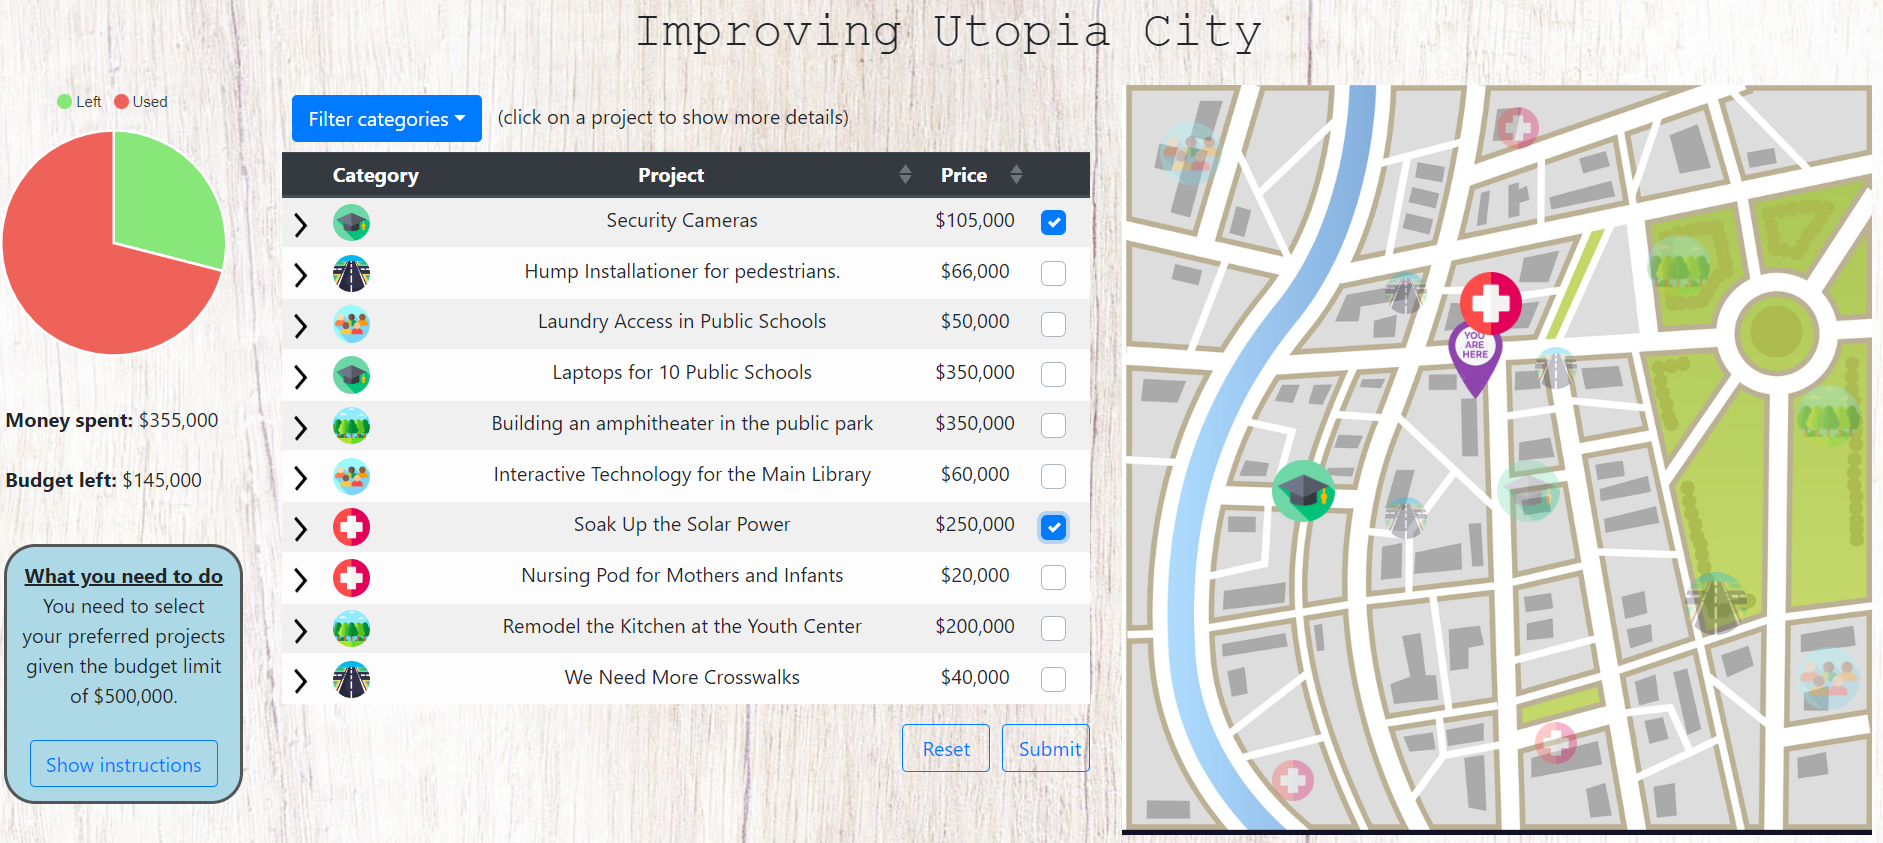
\includegraphics[clip, trim=0 3mm 0 0, width=13cm]{experiment/full system.PNG}
\caption{The GUI shown to participants using the \knap{}  input format (center), showing  the city map (right) and budget (left)
}\label{fig:interface}
\end{center}
\end{figure*}

%In such a scenario, you may be asked to evaluate how much you like a spending plan given your preferences, or how adequate you think a spending plan is given other people’s preferences.
 %Two of the   configurations included ten projects (denoted \textsc{few} \{a,b\}) and two   Each participant was presented with one of the configurations and voted in only one format. 

 
Participants were first presented with a written and video description of the PB voting task. They had to pass a simple quiz about the task in order to proceed. 
Next, participants carried out the voting task 
in their allocated PB configuration.
Each participant was assigned a  (random) location on the city map and   shown the description and location of the projects. 
We expected that a voter's location relative to  the project may affect their   preferences (e.g., people may prefer to vote for a library  close to their current location). 
  



% move to later: In reality, a voter's location may affect their preferences, for example someone may support the construction of a library or park only when they are located close to where they live, or a football stadium only when it is located sufficiently far away.
%We mimic this by assigning participants a randomly drawn location, and visualizing this, together with the locations of the proposed projects, on a hypothetical city map.  
 




 Figure~\ref{fig:interface} shows the interface  presented to participants who were asked to cast knapsack votes. 
 The left-most column shows the instructions and an indication of what fraction of the budget remains to be allocated. The center column shows the category and title of each proposed project, and a participant can click on a project to see a more detailed description. The right-most panel shows a map of the city on which the locations of the voter and the projects are marked (hovering over a project highlights its location). The other interfaces used in the study may be viewed in Appendix~\ref{app:interfaces}. Project costs was only displayed for \points{} and \vfm{}, where it is needed to form a vote. % which require it show the projects cost). %\cref{app:interfaces}. 
 %In the left side of the screen, they are shown the projects they can choose from and which category it belongs to, and in the right side, there is a map which shows the location of the participant and the location of each of the projects.

 %%Each participant got one of them in random (knapsack interface can be seen in Figure~\ref{fig:interface}, the rest of the input formats be seen in the supplementary material).
%Appendix~\ref{app:interfaces}).

%In addition, the participant is presented with one of four sets of projects, either with 10 projects (noted by elections 3 and 6) or 20 (noted by elections 7 and 8). The exact projects in each election can be seen in the supplementary material).
%Appendix~\ref{app:elections}).

% After casting their votes, the participants were presented with  a consistency test with three multiple choice questions 
% %(will be referred by consistency test) 
% which test whether they understood the task and thought about their choice or just rushed through the task. This way, it is possible to analyze the data only from participants which gave some thought on their response.
 
 After   submitting their PB vote, participants were required to answer several consistency questions about their vote that were  designed to identify voters who vote randomly or carelessly (exact questions can be found in Appendix~\ref{app:consis}).  Finally, participants were asked to complete a short survey about their subjective experience of voting in the assigned format. They were asked to rate (on a scale of 1 to 5) how easy they found the task, how much they liked the user interface, % and the map functionality \kg{what was this functionality?},
  how   expressive  they found the input format, 
 and how much the project categories and their location on the map    affected their decisions (exact questions can be found in Appendix~\ref{app:survey}). 
 
 Participants were rewarded a  fixed sum    for participation and  received a 75\% bonus for passing the  consistency questions.
 %Participants were rewarded a  fixed sum of 40\textcent{}   for participation and  received a 30\textcent{} bonus for passing the  consistency questions.
 IRB approval was obtained from the corresponding institution.

%%%%%%%%%%%%%%%%%%%%%%%%%%%%%%%%%%%%%%%%%%%%%%%%%%%%%%%%%%%%%%%%%%%%%%%%%

\section{Effect of Input Format on Voter Experience}
%\section{The usability of different input formats}
%\rf{Why do we have two titles one after the other here? shouldn't be at least some text between them? does the second title should be subsection?}\gb{just two options for the section title, we should comment one out}


%We attempt to further our understanding of 
We investigate the practical effects of using different input formats by comparing  the experiences of voters using the respective input formats.

This comparison has several components. Objectively, we record the time that it takes a voter to complete each of the first three stages of the task (completing the tutorial, answering the post-tutorial quiz, and casting a vote). % which is known to be a reasonable proxy % use this time as a proxy  
%for how hard the participant found the task \citep{rauterberg1992method}.
We also report the number  of participants who fail the post-task consistency test and argue that a participant's inability  to recall simple information about the vote they just cast is correlated with the participant finding the task taxing, confusing or tiresome. 
More subjectively, we examine participants' self-reported scores from the post-completion survey. 
%In this section we will focus on analysing which input format should be used. We will be doing so while keeping in mind the results from the previous section, where we saw than when using RX, the input format used, have very small impact on the outcome, therefore, we will focus on the usability of the input formats. In order to measure this, we look at at objective and subjective indicators, which are inferred from the data collected from the survey the participants submitted.

% For the objective indicators we will first look at the results from the consistency test. This test checks how well the participants understood the task they were given, in addition to how much they paid attention and understood what they did in the voting phase.
% Second, we record how long it took the participants to do each part in the experiment, which is an indicator on the cognitive burden it created.

 
%As for the subjective indicators, we gave each participant at the end of the experiment a short survey that checks how usable the input format was from their perspective.

%\subsubsection{Objective Indicators}

\subsection{Response Time}
The time it takes to complete a task is a recognized  proxy for  the cognitive burden  or difficulty of the task  \cite{rauterberg1992method}.  
%
The average time to complete each stage of the experiment is visually represented in  Figure~\ref{fig:time}.  Results in this section are averaged across elections and the conclusions do not change when looking at any individual election. %\gb{May be worth just looking at times for large vs small to see if there is anything interesting}

Participants voting in  the \vfm{}   format are consistently slowest to complete each stage of the experiment, suggesting that voters find \vfm{}  very hard to use. Based on the time it takes to cast a vote,  \points{} and \tapp{} are the next hardest formats to use. In the former case, we believe this supports the idea that asking voters for cardinal utilities is generally not feasible; in the latter, it  highlights the complications that sprout from  \tapp{} requiring cross-voter normalization  (as well as the fact that \tapp{} is a relatively niche format which voters are unlikely to have encountered before). 
%Interestingly, participants take a long time to complete th

% As can be seen, ranking-value-money takes the longest to learn, to answer the quiz and to cast a vote. This implies on very high cognitive burden this method create, being hard to learn and use.
% For the other formats, the learning time and casting time is ranked as follows: K-approval, Knapsack, Ranking-value. Lastly, Threshold was quicker to learn compared to Utilities, but took longer to cast the vote.
%\gb{We should mention/show that the trends are consisitent across elections}

Voters found \kapp{} the easiest to use, followed by \knap{} and \rank{}.

\begin{figure}[!h]
\begin{center}
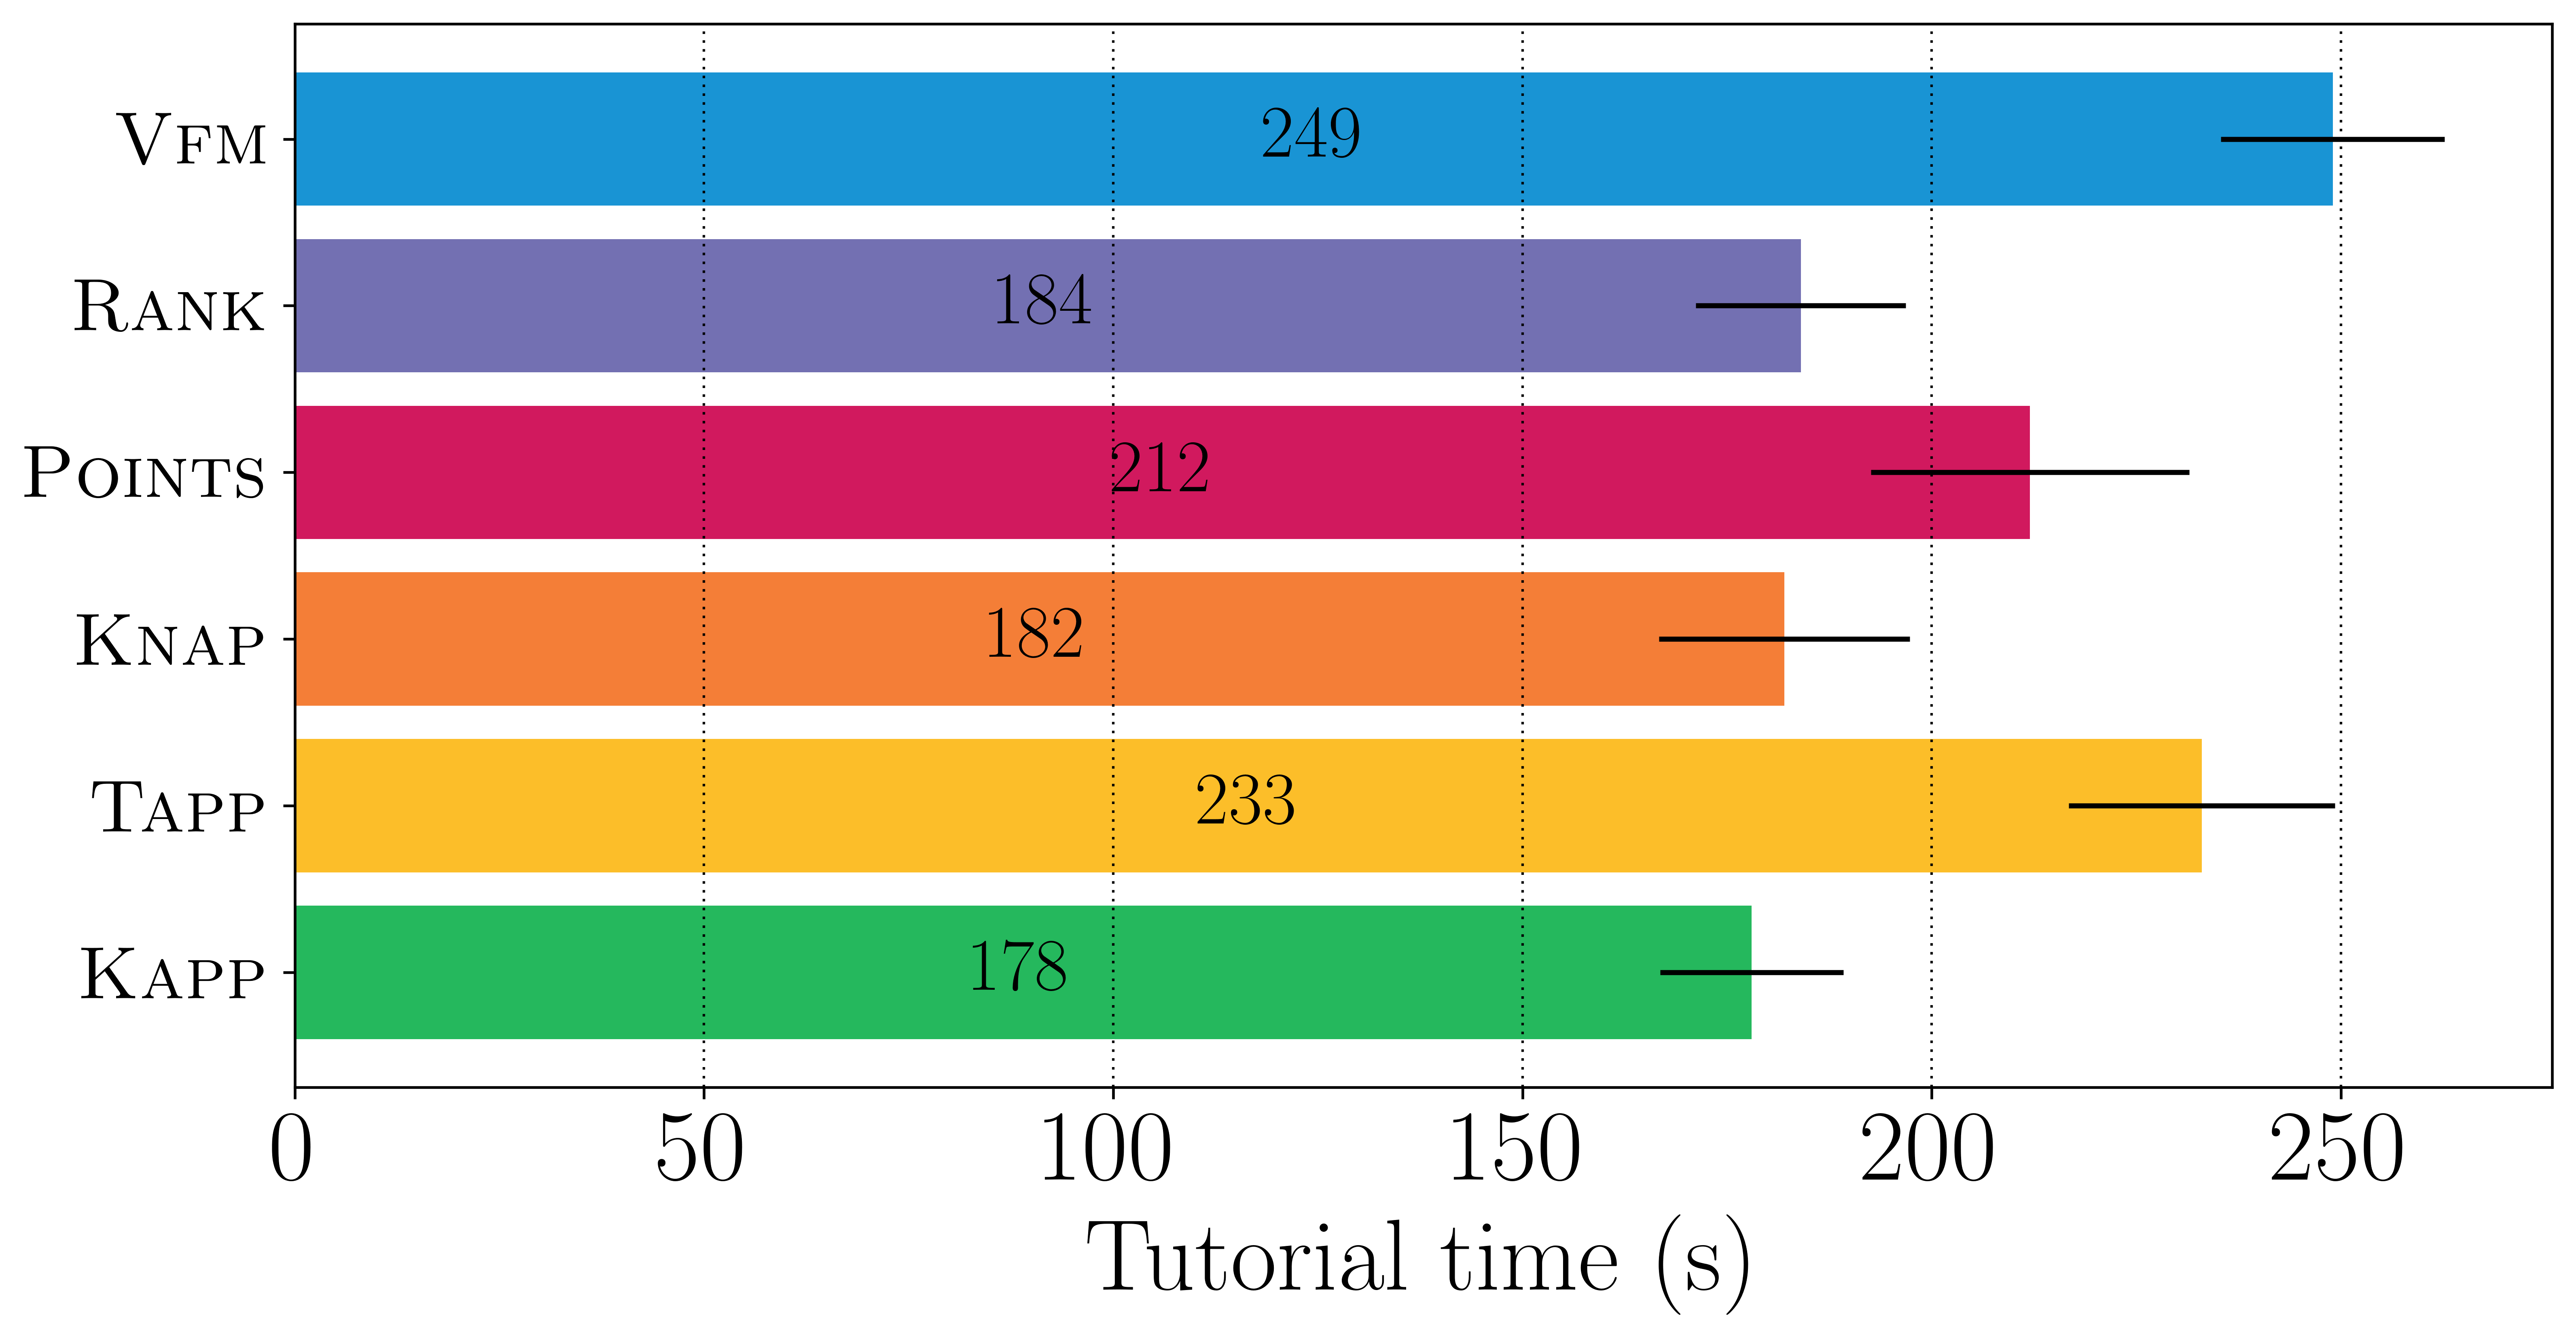
\includegraphics[width=8.5cm]{experiment/tutorial_time.png}
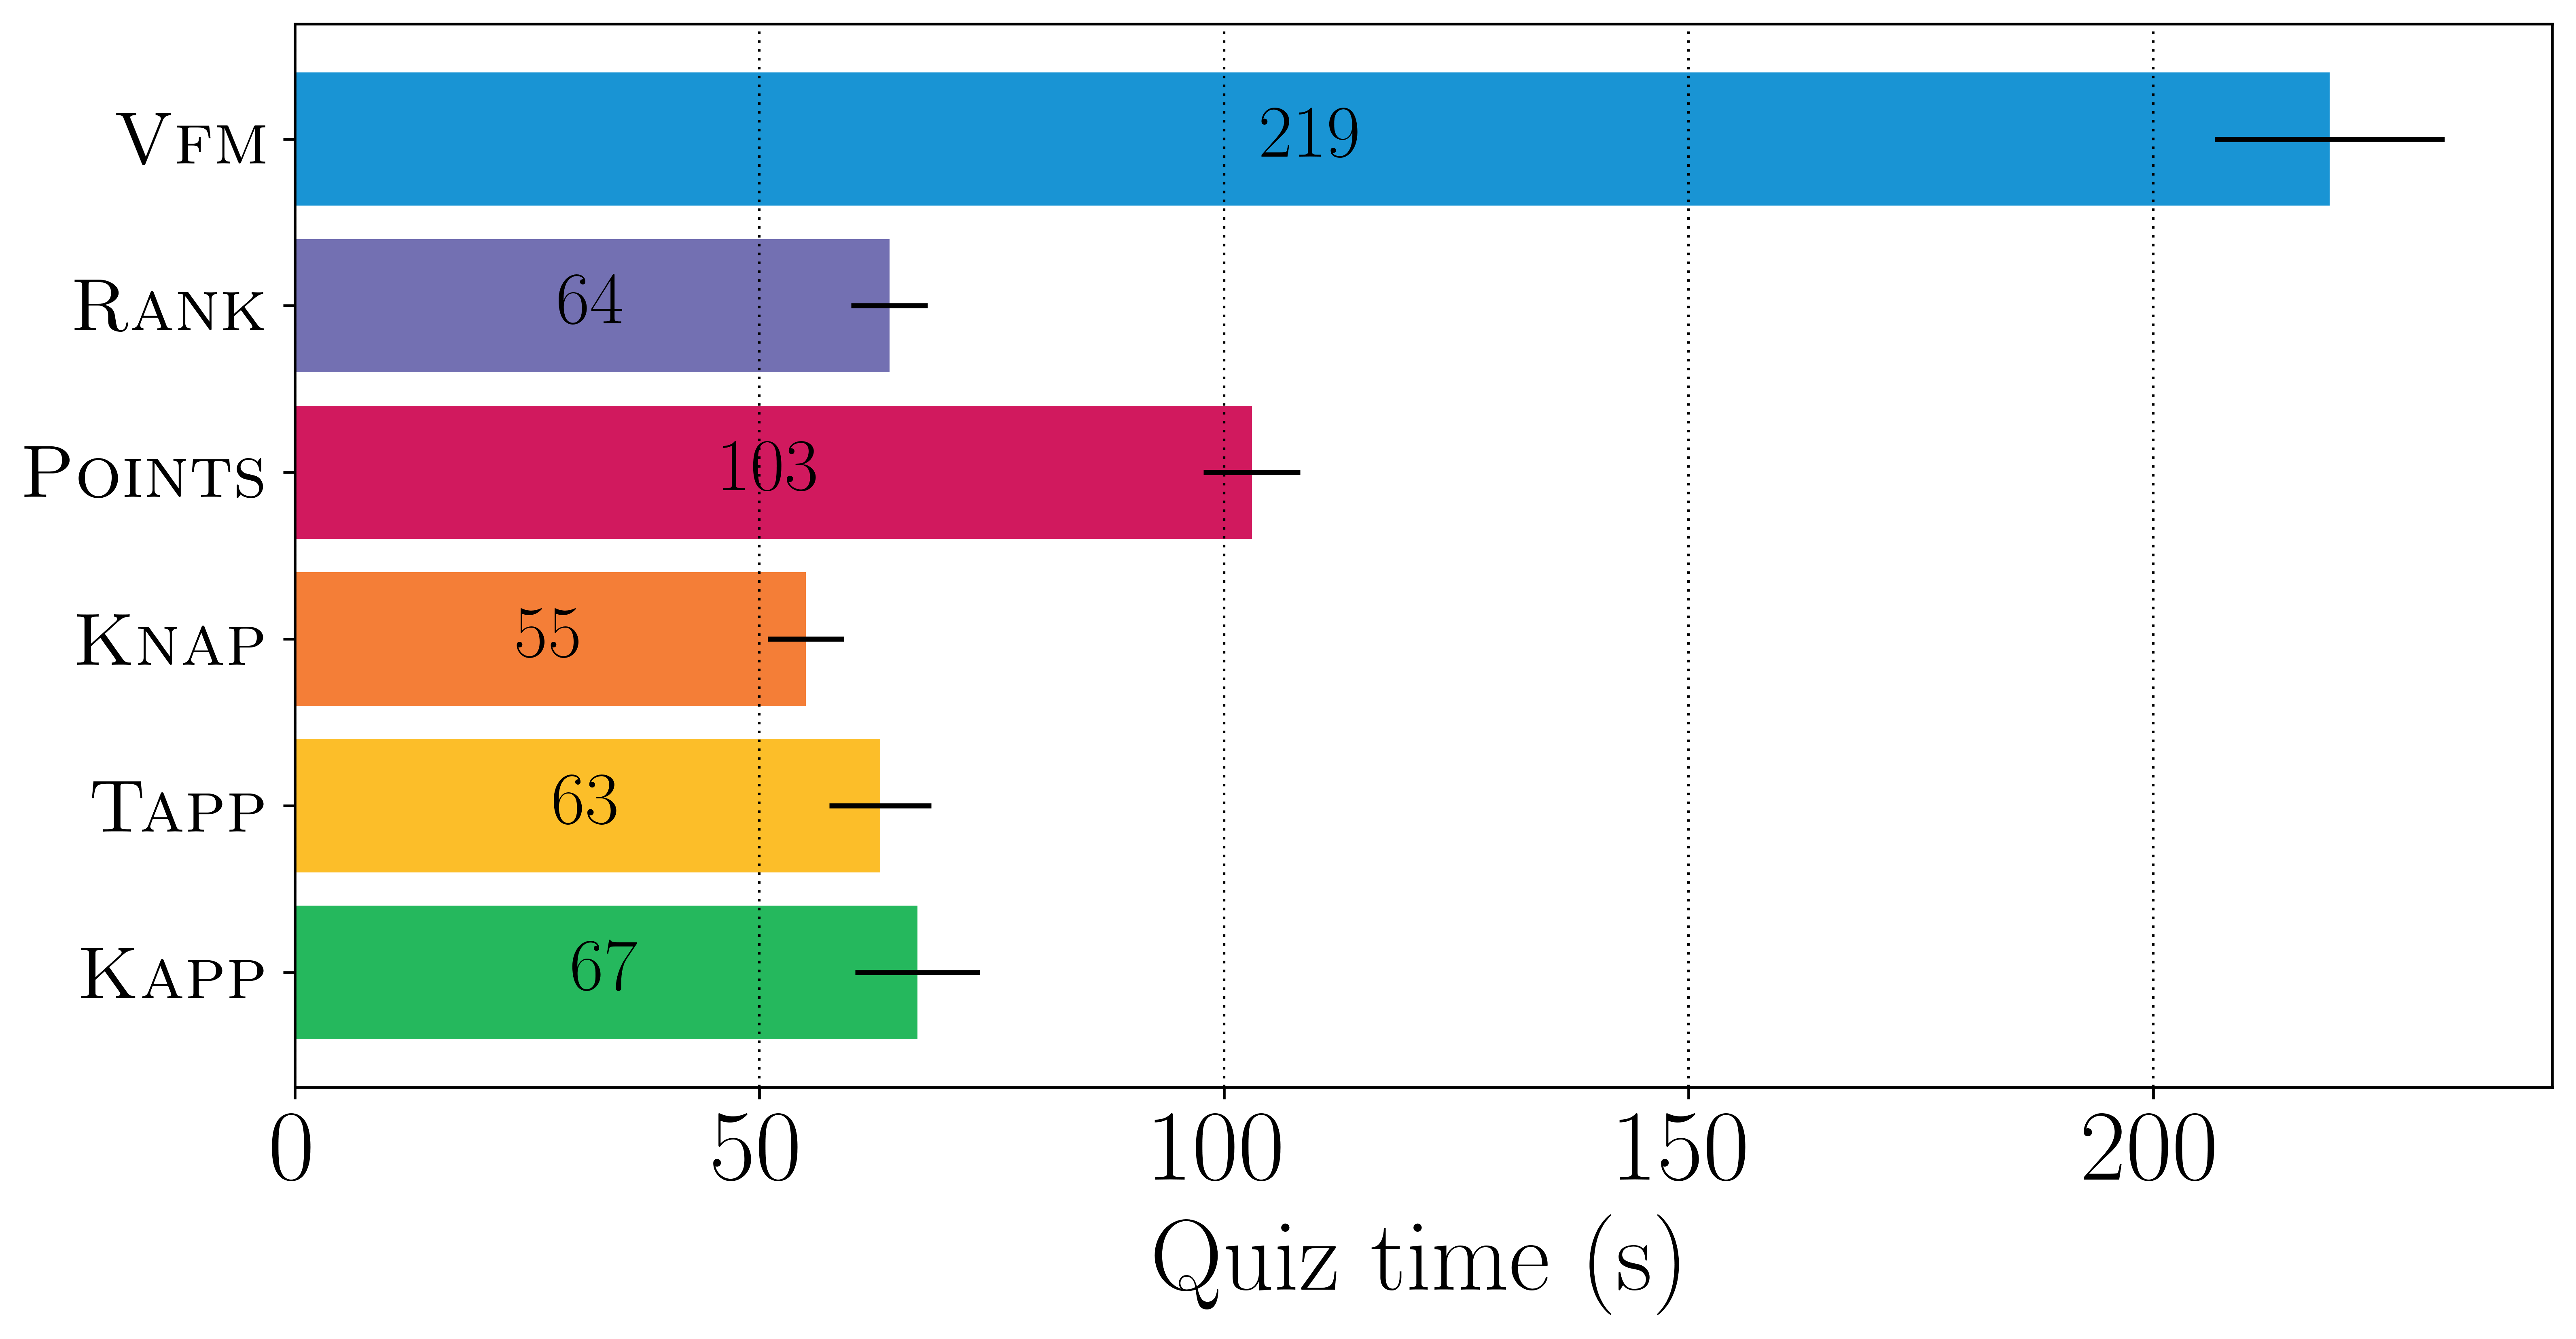
\includegraphics[width=8.5cm]{experiment/quiz_time.png}
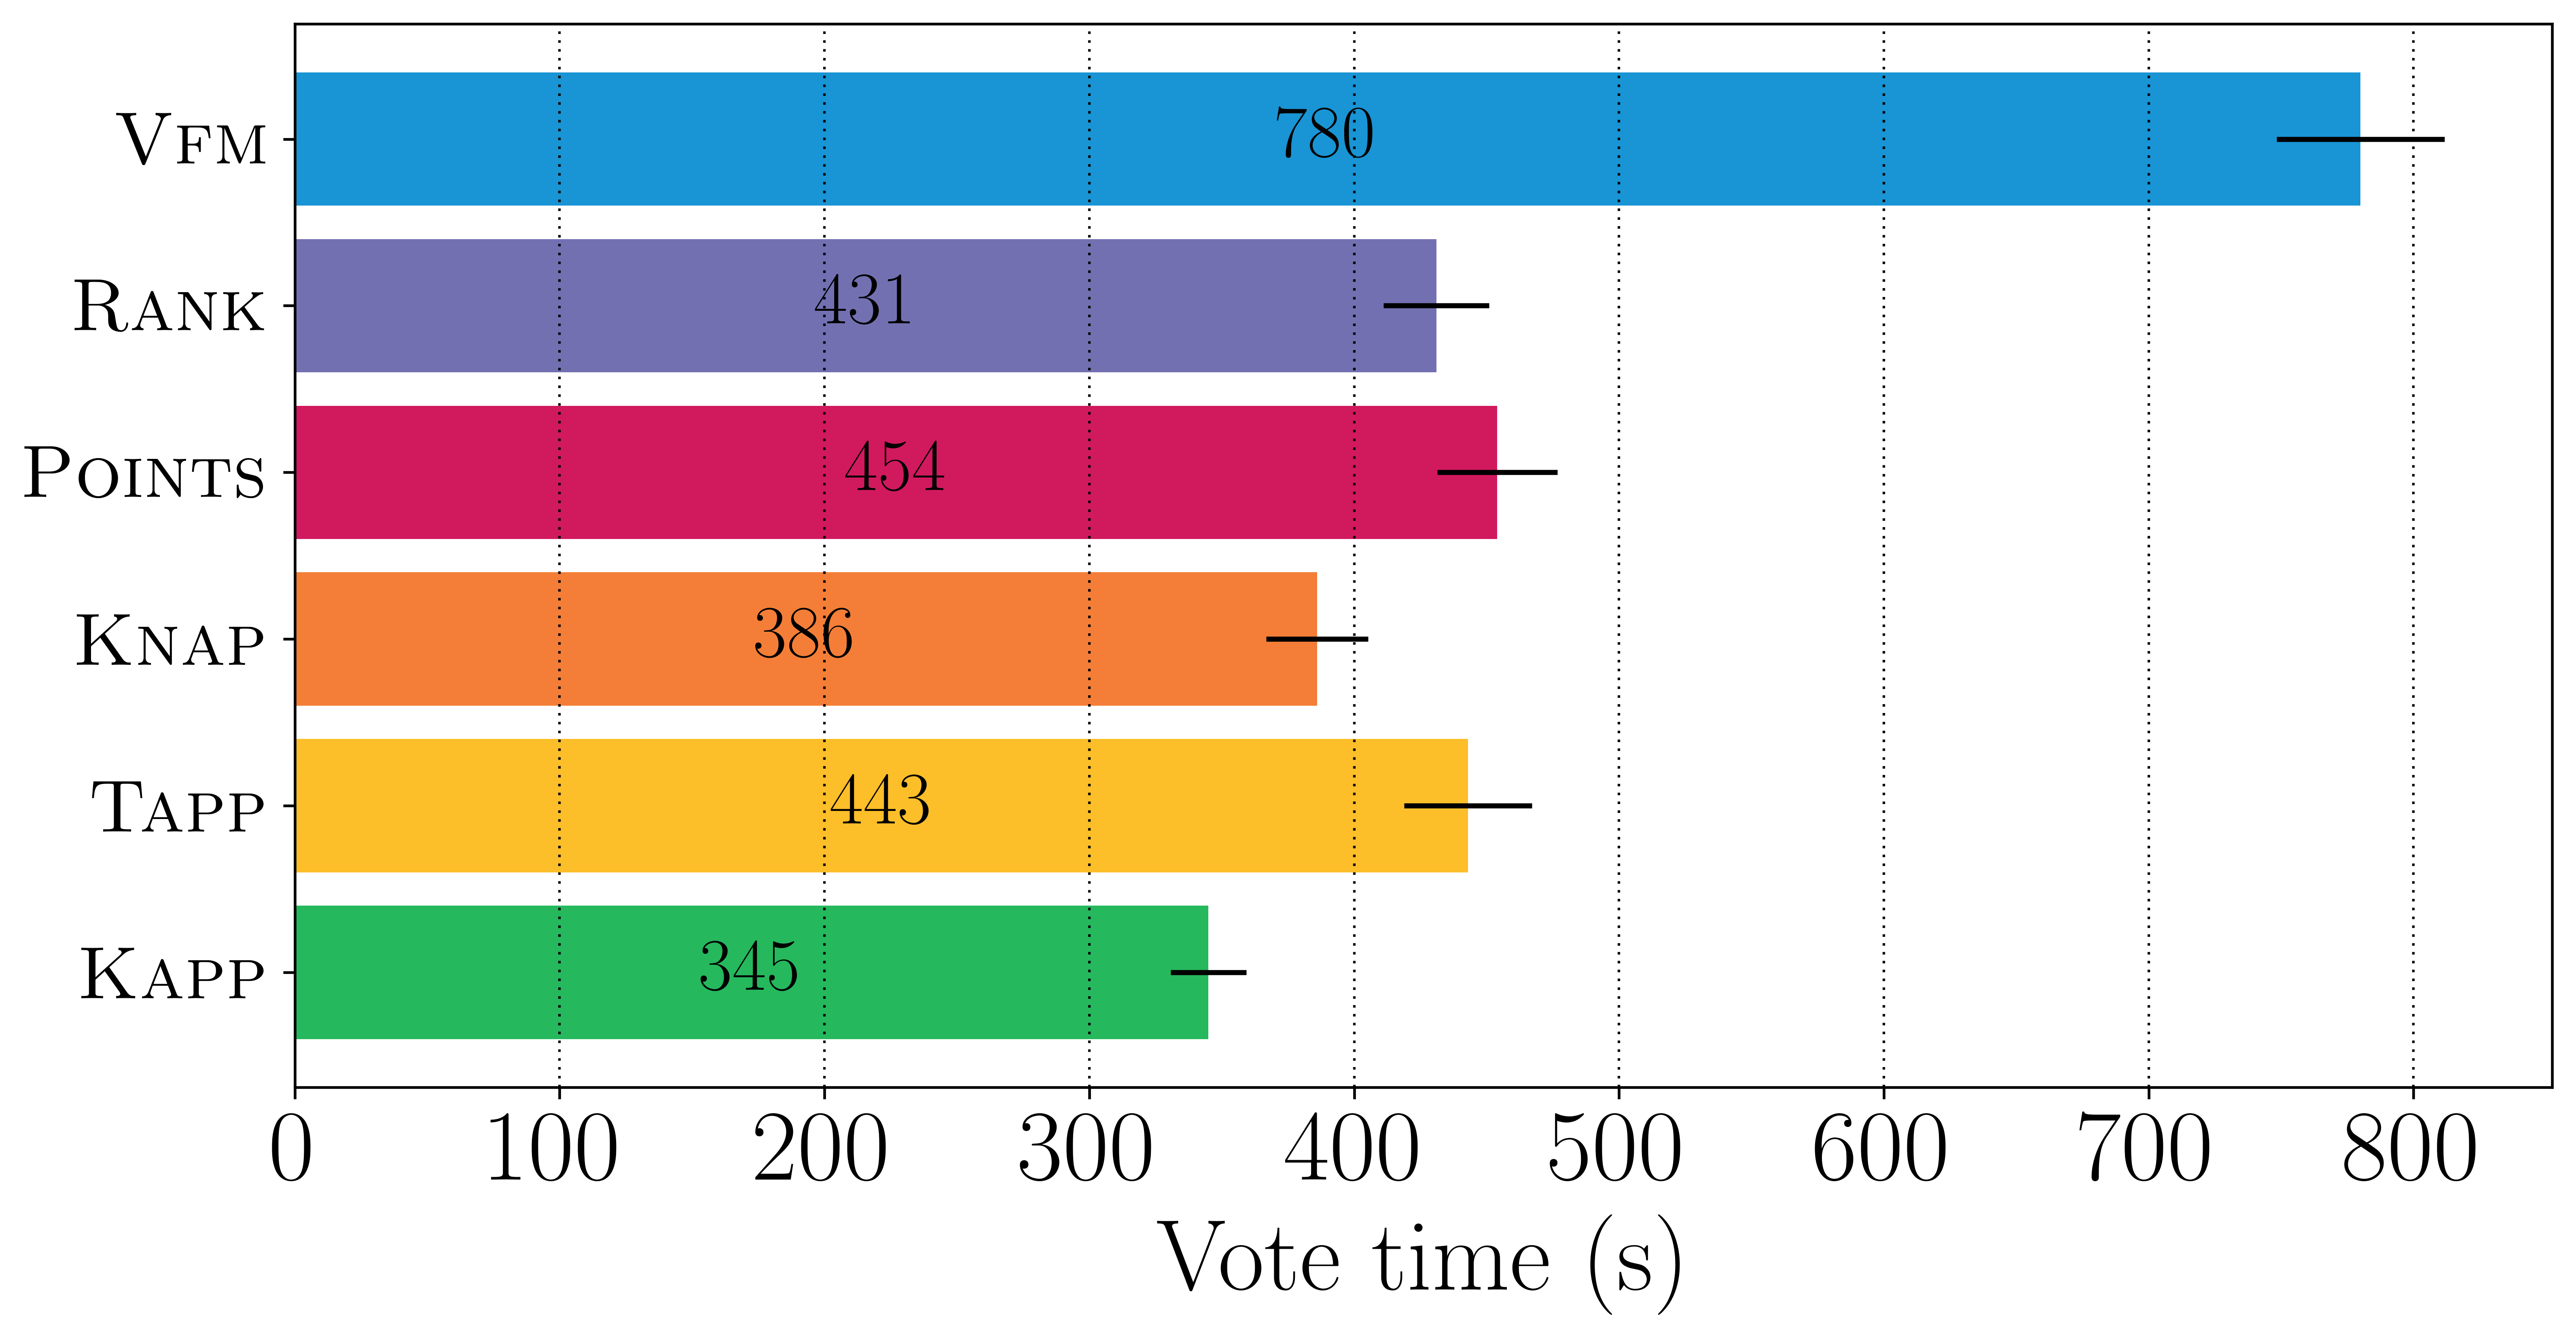
\includegraphics[width=8.5cm]{experiment/vote_time.png}
\caption{Average time ($s$) to complete each stage. 
}\label{fig:time}
\end{center}
\end{figure}

\subsection{Consistency Checks}

%\emph{\textbf{Consistency.}}
%\gb{i want to call this something else to distinguish from other paper's different consisitency} 
Of the roughly 75 participants  recruited for each of the 24 configurations of the experiment, on average 58 passed the consistency test. 

The consistency test  is designed to check whether the participant can recall simple information about the recently completed task. 
%
There are several reasons why a voter may fail the test. For example, they may answer randomly in order to complete task quickly,  become  distracted  if the task is too tiresome, or confused if the input format is hard to understand. As such, we  treat this as another signal about the difficulty of expressing  preferences in a given format. 


%Diving into the different configurations, one can see that the percentage of consistent voters changed between different input formats, however, it was virtually identical across different project sets. The numbers of the consistent participants for the configurations can be found at the Appendix.


% \rf{I think we can remove this figure completely here, and instead just say we had about 300 participants for each input format and instead show a small table with the consistency percentage. What do you think?}
% Figure~\ref{fig:consistency} represents the total number of participants in each input format as well as those who failed the consistency test, aggregated across elections.\footnote{The overall rate of passing the consistency test is virtually identical across elections, see the Appendix for further details.}
%From the consistency results, we can infer whether a certain input format or the amount of projects affects on how hard was a configuration to the participants. The results can be seen in Figure~\ref{fig:consistency}.



%As can be seen in Figure~\ref{fig:consistency}, While there is different amount of consistent participants for different input formats, the suggested projects or the number of possible projects have no effect on how consistent participants are. From those results, we can say that participants had the least difficulty in the ranking formats, following by the approval formats and finally the utilities format which as we claimed earlier give the most information, however, take the most cognitive burden on the participant.

We  compare the rate of passing the consistency test across input formats. 
Participants using the ranking-based formats were most consistent, followed by the approval-based formats.  We speculate that the high consistency of \vfm{} is, at least in part, thanks to the inordinately long amount of time voters spend considering their votes. Users of \points{} were comfortably the least consistent, which  supports earlier evidence that providing cardinal utilities is a challenging task.

There was virtually no variation in the rate of passing the consistency test across the four elections. A complete breakdown of the results may be found in Appendix~\ref{app:comparison}. 

% \begin{figure}[!ht]
% \begin{center}
% 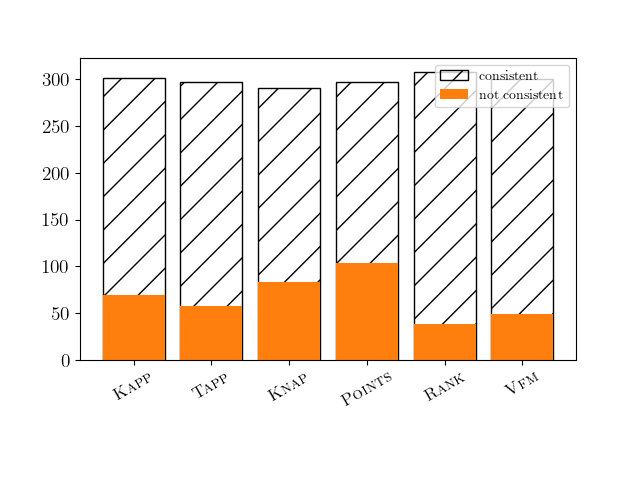
\includegraphics[width=7.5cm]{experiment/format_consistency.png}
% %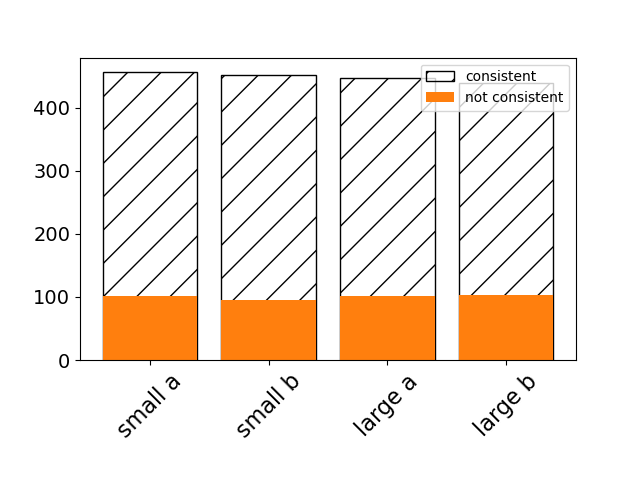
\includegraphics[width=7.5cm]{experiment/election_consistency.png}
% \caption{The total number of  participants who vote in each format, as well as the number that fail the consistency test.  Numbers are aggregated across elections. 
% %\gb{should label elections properly eventually, not 3,6,etc. }
% }\label{fig:consistency}\rf{I think figure can be removed, read comment in the consistency subsection}
% \end{center}
% \end{figure}


\subsection{Self-Reported Voting Experience}
In addition to the time it took participants to complete the task and how much they could recall about their submitted preferences, we also expressly asked them to rate various aspects of the experience on a scale of 1 to 5. %we had a survey where we asked the participants about their experience with a certain input format. 
Survey results are summarised in  Figures~\ref{fig:feedback} and \ref{fig:cat_map}.
Results for the questions omitted from this discussion may be found in Appendix~\ref{app:comparison}.
In order to find statistical significance, we first used Kruskal–Wallis test to show the input formats give different results, followed by the Dunn test for post hoc comparison.
All of the survey questions   gave $p < 0.004$  for the Kruskal test. The Dunn test evaluated statistically significance   at the $p < 0.05$ level.
%\gb{Should Dunn be capitalised? Also, I don't understand these two sentences at all}\rf{I'm not sure about Dunn, as for the sentences, what I meant that I first ran kruskal on all questions and got significant results using pval of 0.004. Next, for each pair of questions I ran Dunn, saying that the results are significant for pval of 0.05. We should rephrase the sentence so it is clear for the reader.}
% Statistically significance is tested using a two-sided   Mann-Whitney tests at the $p < 0.05$ level.
% \gb{I'll send an email about this}


\textbf{Ease of use}  We asked the voters how easy they found the voting task. Unsurprisingly, participants found \vfm{} significantly harder to use than any other format. \points{} was rated as quite easy to use despite being one of the more time-intensive formats. \kapp{} was rated as significantly easier to use than all other  formats except \points. 

%\textbf{User interface} - We asked the participants how much they liked the interface. Ranking-value-money is significantly worse than any other input format, while in contrast, k-approval is significantly better than all other input formats except for utilities and knapsack.

\textbf{Perceived expressiveness} We asked the participants how well they felt their vote captured their preferences. 
%The results here are a bit surprising, ranking-value-money is significantly worse than all other formats, even through the same vote is cast as in ranking-value. In addition, we see that k-approval achieve the highest capture (significantly compared to threshold, ranking-value-money and utilities). This is surprising as approval voting let the voter the least power to express themselves, compared to the other formats.
Participants found \kapp{} to be most expressive and, in particular,  significantly more expressive than  \tapp, \vfm, and \points. It is somewhat surprising that \kapp{} was rated as more expressive than \points, since you can infer a \kapp-vote from  your \points-vote; we speculate that the relative complexity of  \points{} explains part of this phenomenon. It is also possible that participants conflated expressiveness and ease of use, or failed to consider alternatives to the format presented to them. % Another possibility for this is that participants misunderstood expressiveness (and projected ease of use on it) or they just did not consider there are other alternatives for \kapp{}.
\vfm{} was perceived to be least expressive by some margin. Again, the  difficulty of using \vfm{} and the fact that voters are forced to explicitly consider project costs may have contributed to the perception that it is less expressive than \rank, which also asks for a ranking of alternatives.  


\begin{figure}[!h]
\begin{center}
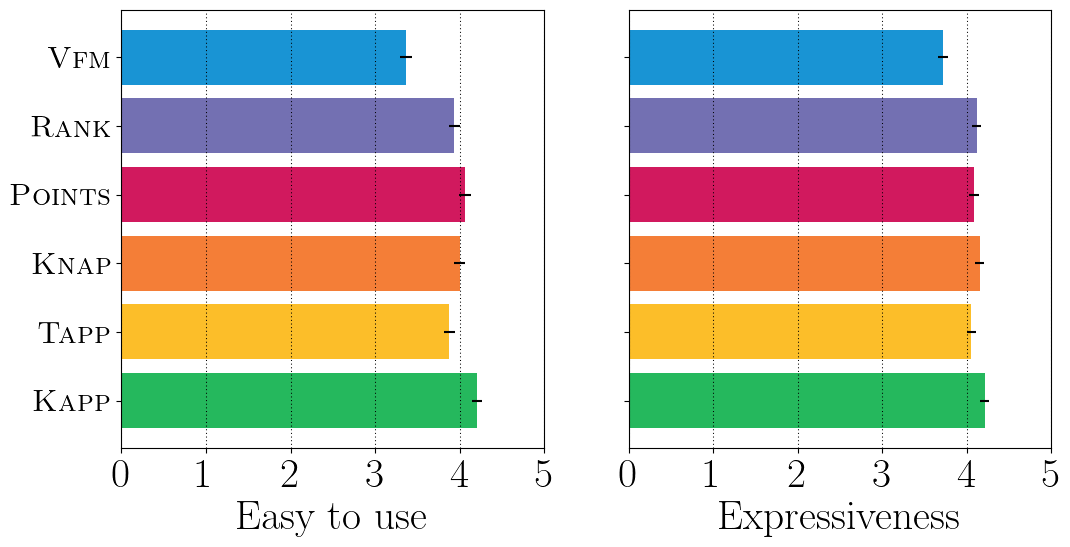
\includegraphics[width=10cm]{experiment/survey1.png}
\caption{The average feedback for each input format.
}\label{fig:feedback}
\end{center}\vspace{-3mm}
\end{figure}

\begin{figure}[!h]
\begin{center}
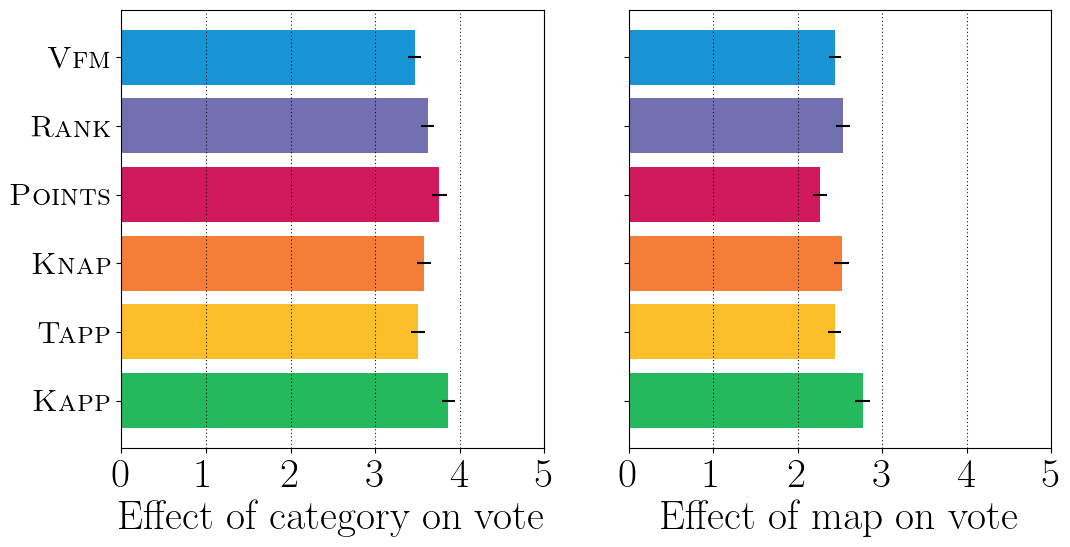
\includegraphics[width=10cm]{experiment/survey2.png}
\caption{The average effect of the categories and the map.
}\label{fig:cat_map}
\end{center}\vspace{-5mm}
\end{figure}

% \begin{figure}[!h]
% \begin{center}
% 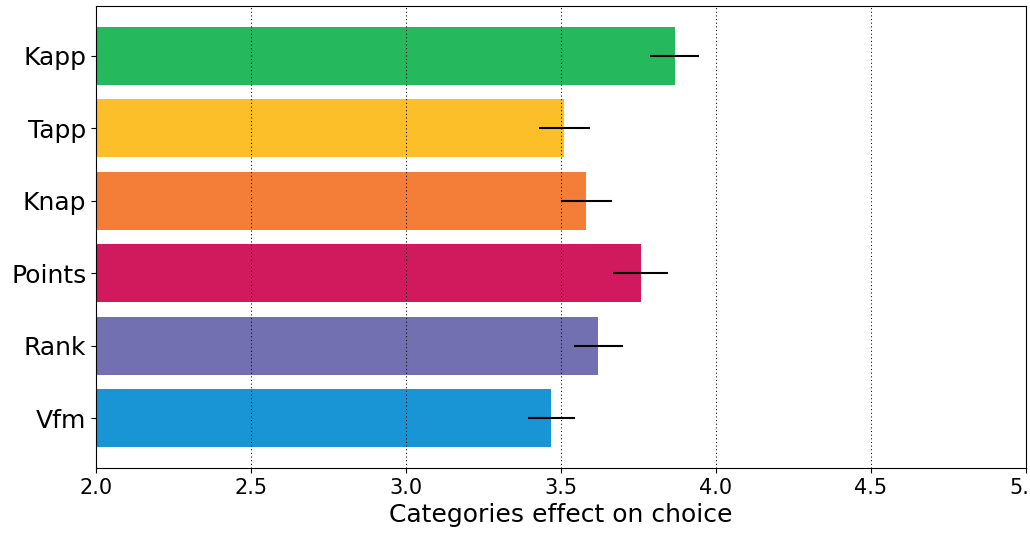
\includegraphics[width=7.5cm]{experiment/survey3.png}
% \caption{The average effect of the categories.
% }\label{fig:categories}
% \end{center}
% \end{figure}

\textbf{Effect of additional information}
Projects were assigned to one of five categories (e.g.\ transport or education) and given locations on a city map. Two survey questions asked about the extent that project categories and the map influenced participants' preferences. These results are summarised in Figure~\ref{fig:cat_map}

Participants using \kapp{} were influenced  more by project locations than any other group. Similarly, \kapp-voters paid significantly more attention to project categories than all other groups except \points-voters. 
It may be that the \kapp{} format was easy enough to understand and use that it freed participants up to consider additional, non-core information about the projects and   election in their decisions. 

%%%%%%%%%%%%%%%%%%%%%%%%%%%%%%%%%%%%%%%%%%%%%%%%%%%%%%%%%%%%%%%%%%%%%%%%%

\section{  Effect of Aggregation Method on Outcome}  


%\section{Effect of input format on outcome}
\label{sec:aggregation}
%Beyond user experience, an input format may be preferred because it leads to better outcomes.  
In  this section we  analyze the effect of aggregation methods  on the outcome of the elections.
%For each of the input formats, we aggregated results using greedy aggregation or the \mes{} approach. 

%In this section we will focus on two aggregation methods described in Section~\ref{sec:prem}, greedy and RX. We will use the data collected in the experiment in order to show how the outcome is affected from using different input formats when using greedy aggregation and RX.
%The input format which consistently leads to better outcomes (however that is defined)  can be argued to be superior. 
%A good input format should be expressive enough that it is possible to identify the best projects

% An aggregation method is a function from a set of votes in some input format to a set of chosen projects that doesn't exceed the budget.


%move to intro%A good input format should  capture enough information so that it is possible to identify the best projects. 
%We investigate whether particular formats tend to result in better outcomes. 

% In this paper we compare  two aggregation methods.
% Greedy aggregation selects projects in decreasing order of total reported utility until the budget is depleted. This is the most common voting rule used in real world PB settings.

% \rf{TODO: need to use either equal shares or RX; also improve descriptions of RX}
% The method of equal shares~\citep{peters2021proportional} is a theoretically attractive alternative to greedy aggregation which divides the budget among voters and allows voters to collaborate to purchase commonly supported projects until their budget is depleted.
%The method of equal shares~\citep{peters2021proportional} divides the budget among voters and allows voters to collaborate to purchase commonly supported projects until their budget is depleted. The method of equal shares is a theoretically attractive alternative to greedy aggregation  which is yet to be used in practice.

% In this section, we will start the analysis by looking at methods to aggregate the votes in order to choose which projects to fund.
% As mentioned in Section~\ref{sec:intro}, the method that usually used in the real world is greedy aggregation, however, this method have several disadvantages. We will compare it to Rule~X~\citep{peters2021proportional} (RX), showing why it is recommended to use it instead of greedy aggregation. 

% Both aggregation rules require cardinal utilities, which is defined as in Section~\ref{sec:prem}.
%hose two methods, based on numeric utility for each of the projects, thus, we will start by explaining how the different formats are represented in utilities. 
% For the knapsack and approval formats, we assume binary utilities; the number of points distributed to a project is directly treated as utility; rankings are converted to Borda scores. %each approval worth score of 1 and 0 other wise. For the ranking formats, we use Borda score, and finally for utilities the score is the utility given for a project.

\subsection{Stability} 

%To do so, for each election and input format, we will pick uniformly at random a subset of voters and aggregate them to get an outcome. This process is repeated 200 times, counting the percentage of instances where each project was selected. 
 

% In the greedy heatmap (bottom), we see the exact opposite results from \mes{}. First, the outcome can change a lot, depends on the voters that took part, and therefore, less likely to represent the full population. Second, while there is some similarity in the projects distribution across input formats, there is a dependency between the outcome and the used input format (which supports the results in Figure~\ref{fig:welfare}).
% Lastly, greedy aggregation does fund sometimes expensive projects, leaving less funds for other projects. This is caused because the aggregation method ignore the cost, taking only the amount of votes into account.

% The results for the rest of the elections show similar trends and can be found in the supplementary material.
%\footnote{We also ran the experiment sampling only 10 voters each time,  which yields less correlated input profiles. The same  general trends were present.} 

We first study the   stability of the different aggregation methods. %We should prefer aggregation methods that meet the following criteria 
We say that an aggregation method is stable when the outcome of the election is:
\begin{enumerate}
\item Robust to the choice of input format. This allows the organizers to freely select an input format without fear of affecting the outcome of the election (or default to a format voters find easy to use). 
\item  Robust to partial participation.   Voter turnout may be low in real PB elections, ideally the outcome of the election is not drastically affected by the (non-)participation of a small group of voters. 
%This is important because in   real world PB instances, we cannot control the number of voters that participates, and voter turnout is typically low.
% Therefore we should prefer aggregation methods that are less affected by 
\end{enumerate}


In this experiment, we first repeatedly sample $n'=40$ participants per configuration, and aggregate the resulting vote profiles using greedy aggregation and \mes{}. This process is repeated 200 times.% (enough for convergence). 

The fraction of repetitions in which each project is funded in each configuration is summarized in a heatmap in Figure~\ref{fig:heatmap}. The top row of results corresponds to greedy aggregation and the bottom row to \mes. Within each panel projects are ordered in order of increasing cost, and the cells range from white (meaning the project is never funded) to black (always funded). 



% To apply the aggregation methods to the input profiles from the user study, we created PB instances by
% %sampling the votes from participants in the user study. Specifically, we  
% randomly sampling  the votes of participants  in every input format.  We subsequently  applied the Greedy and  \mes methods for each of the PB instances. We repeated this process 200 times, yielding  200 
% outcomes for each aggregation method and input format, calculating the percentage of instance each project was selected. 


% The results for sampling 40 voters is shown in 
% Figure~\ref{fig:heatmap}. The figure shows 
% a heatmap describing the fraction of times that each project gets funded across repeated applications of each aggregation method, 
% %Each panel has a row for every input format and each row has a cell for every project (projects are ordered by increasing cost).  
% %The intensity of the cell corresponds to the fraction of times that the project was funded in the sampled elections of the corresponding input format, 
%  from black (never funded) to white (always funded). 
% % Each column of panels correspond to a different election (small-a, small-b, large-a, large-b). The top row of panels summarize the results of greedy aggregation, and the bottom row \mes.


\begin{figure*}[h]
\begin{center}
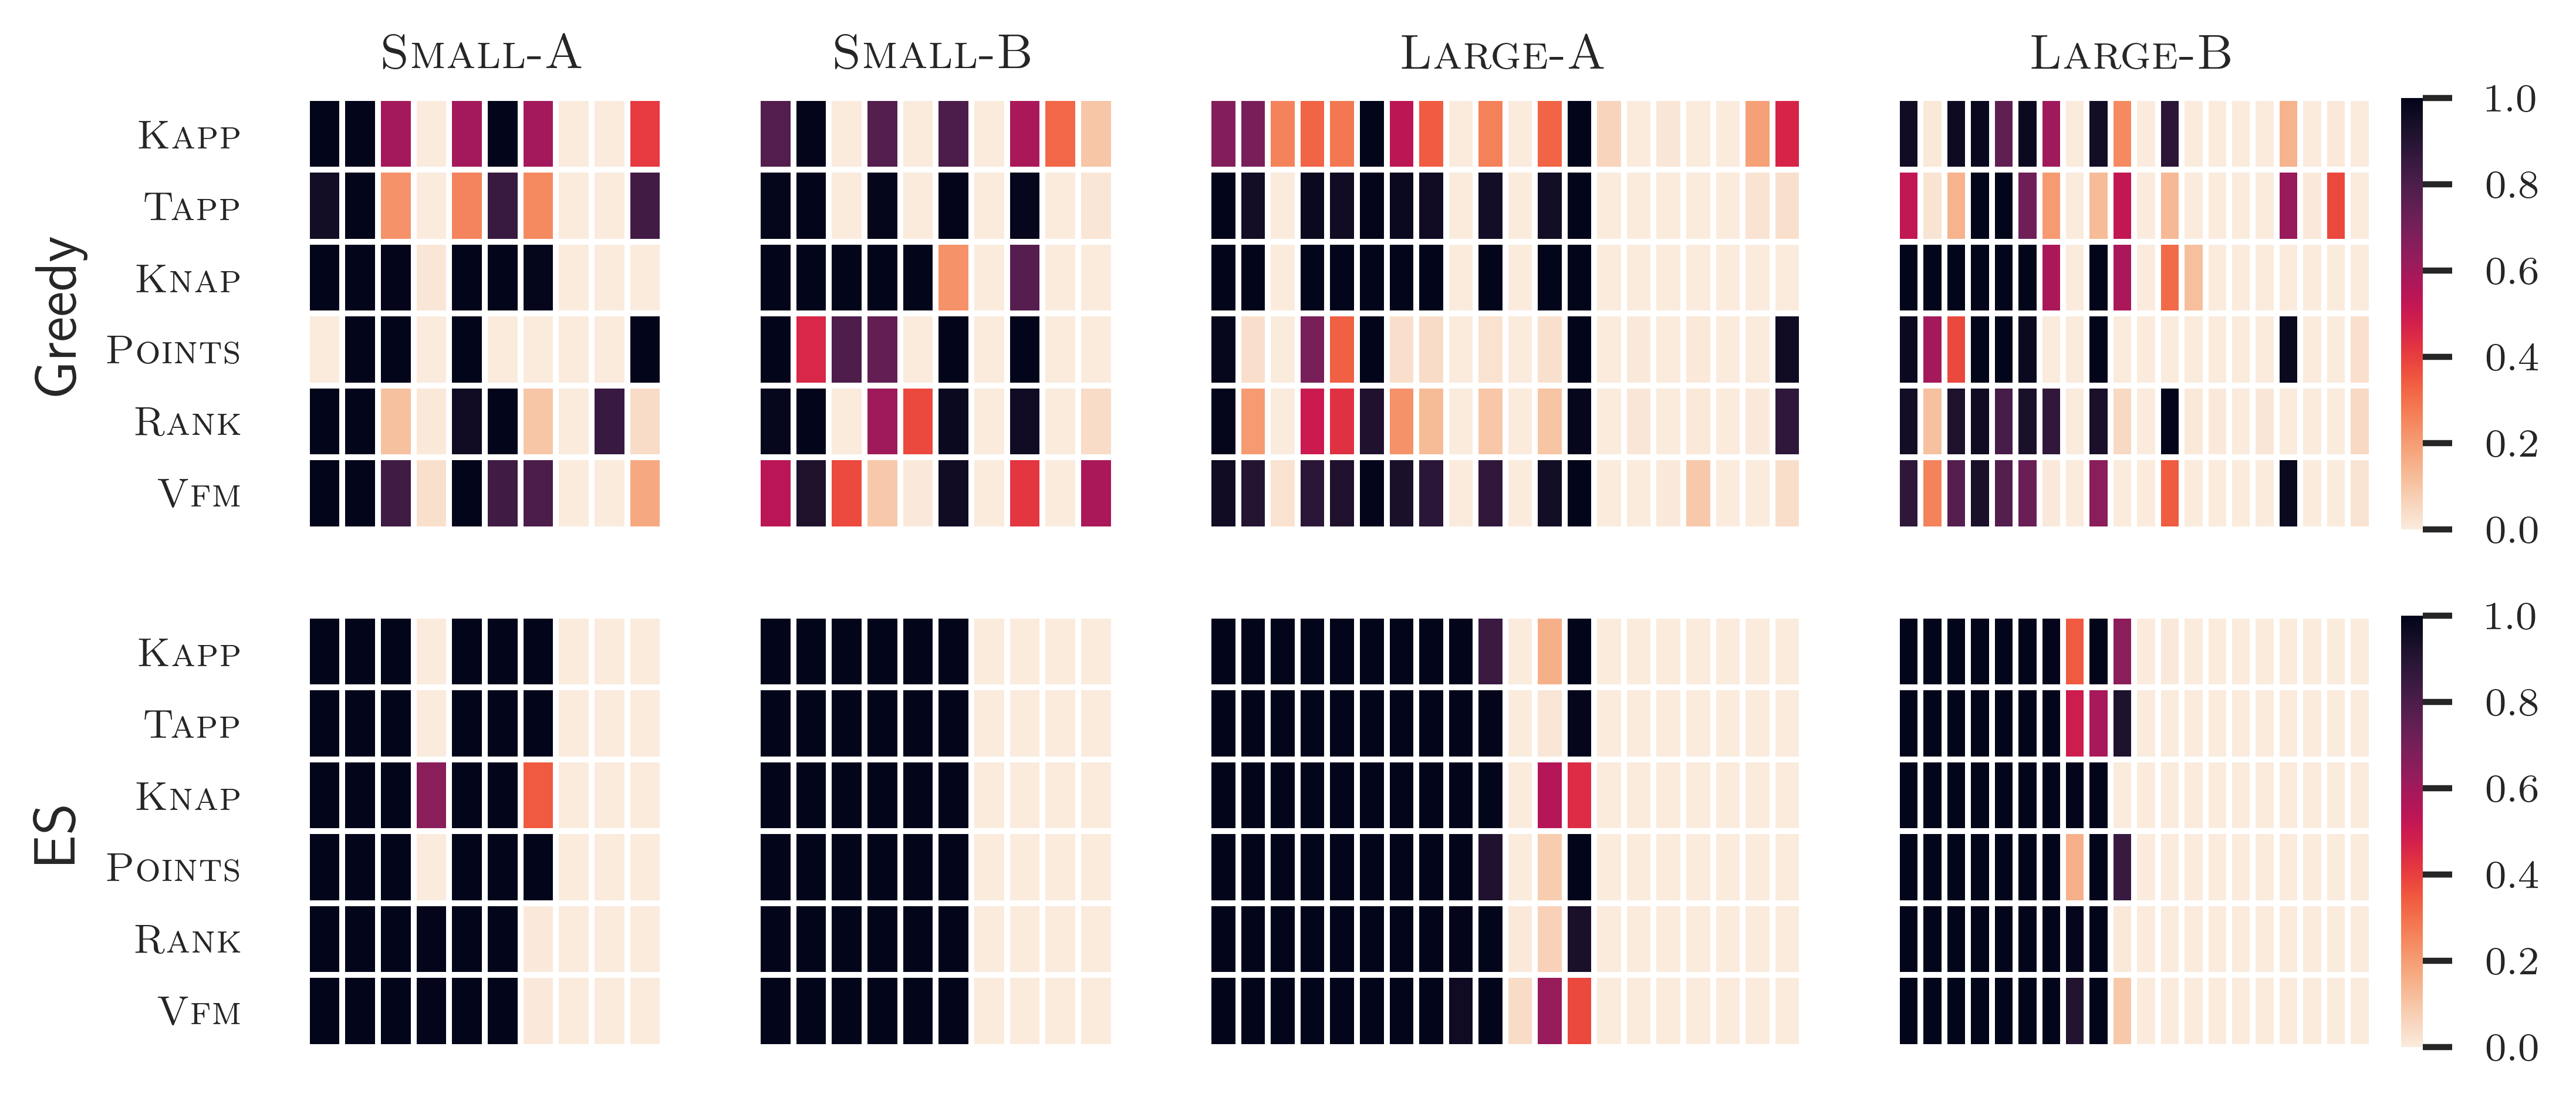
\includegraphics[width=14cm]{experiment/heatmaps.png}
\caption{Stability heatmaps for  greedy aggregation (top) and \mes{} (bottom) in each election. 
%\textsc{Small-A}, \textsc{Small-B} project sets (left) and \textsc{Large-A}, \textsc{Large-B} project sets (right). 
Within each panel each row represents an   input format and each column a project (ordered in increasing cost).
 The intensity of a cell indicates the fraction of instances in which the project was funded.
 %, for a given input format, using greedy aggregation (top) or \mes{} (bottom). A bright cell means that the project is always funded, a dark cell means never funded.
}\label{fig:heatmap}
\end{center}\vspace{-3mm}
\end{figure*}

Strikingly, the outcome of the election is almost entirely unaffected by the choice of input format when using \mes{} --- the majority of the projects are either always funded under every input format or never under any. Greedy aggregation exhibits this property only in rare instances, for example, the outcome of \textsc{Large-A} does not change if the input format is changed from \knap{} to \tapp.  This robustness to the choice of input format remains present when the number of sampled voters is varied $n'\in\{10,20,30\}.$

We also observe in   Figure~\ref{fig:heatmap} that \mes{} is robust to partial participation: it is very rare that the decision to fund a project changes across repetitions when sampling voters at random, i.e.\ under a uniform model of voter participation/abstention. Greedy aggregation does not exhibit this property. 

Of course, since we are sampling 40 votes from (on average) 58 consistent voters the sampled profiles are correlated. We repeat the experiment sampling $n'\in\{10,20,30\}$ voters each time to investigate what happens when the correlation in sampled profiles decreases.
%
To quantify stability under partial participation, we compute the entropy of the outcome for each configuration. Suppose that project $p\in P$ is funded with probability $f_{V,A}(p)$ when aggregating votes cast in voting format $V$ using aggregation method $A$, then $$\text{entropy}(V,A) = -\frac{1}{|P|}\sum_{p\in P} f_{V,A}(p) \cdot \log_2(f_{V,A}(p)) + (1 - f_{V,A}(p)) \cdot \log_2(1 - f_{V,A}(p))$$.

% From the heatmaps we can infer the following. Using  \mes{} to aggregate the votes leads to remarkably stable outcomes. 
% The greedy aggregation method was far less stable. 


% We can infer that the  \mes{} aggregation exhibits many light and dark cells in all rows (i.e., projects are   always chosen or never chosen).  
% This indicates that this method is robust to partial participation and is also robust across the different input formats.
% In contrast, the existence of mixed-shade cells in the Greedy aggregation indicates that this method is substantially less robust than the \mes method.
% %exhibits bright or dark cells across the different input formats. This means 
% % across input formats, 
% % \mes{} outputs relatively the same set of projects for different samples of voters, thus indicating it is robust to partial participation.
% Some correlation is to be expected (we are sampling 40 of roughly the 58 consistent participants), therefore,
% we repeated the experiment when sampling 30, 20 and 10 voters each time, thus lowering the correlation between the samples. We observed similar a similar trend to sampling 40 voters. \kg{why should the reader believe us? We need to include a graph.}
 
 
% In order to provide a quantitative measurement of stability,
% %per input format under partial participation,
%  we computed the entropy of each aggregation method  for each input format. Formally, given the percentage of times each project was selected by a given method (noted by $p$) for some input format, its entropy is calculated by $-\sum p * log_2(p)$.

%across different samples of voters and input formats. 
%This degree of stability is surprising and not shared by greedy aggregation. 



% This is a very attractive feature, voter turnout is typically low so there some benefit to using an aggregation method which  is not particularly sensitive to which exact subset of voters participate in the election. 




Figure~\ref{fig:entropy} shows the entropy for election   \textsc{Small-A} across   input formats for greedy aggregation and  \mes{} aggregation when varying the degree of participation (i.e. the number of sampled voters). 
Unsurprisingly, the correlation between vote profiles decreases and entropy increases  as fewer voters are sampled. 
The entropy of \mes{} is consistently significantly lower than that of greedy aggregation across input formats. We conclude that \mes{} is significantly more robust to partial participation than greedy aggregation. One exception is worth highlighting, the entropy of greedy aggregation with \knap{} votes is fairly competitive with that of \mes. This suggests that if the organizers of a PB election are dead-set on using greedy aggregation and also worried about the effect of partial participation,  \knap{} may be an attractive option.  
%
% The figure shows that the entropy generally increases as we sample fewer voters. 
% The entropy for \mes{} is   lower compared to greedy, and it increases much slower  as we sample fewer voters.  We note two exceptions. First, the \points{} format   begins with very low entropy when sampling 40 voters, but it   increase quickly and gets the worst entropy for 20 and 10 voters. 
% Second, greedy aggregation exhibits  similar entropy to  \mes{} using \knap{} format across  all sample sizes. 
% %Those good results of greedy, happens only for project set \textsc{small}-a, 
For the other three elections,   \mes{} aggregation comfortably outperforms greedy aggregation across all input formats and sample sizes (except similar results for \knap{} in election \textsc{Large-A}). Full results  may be found in Appendix~\ref{app:entropy}. 


%As for the next next trend from Figure~\ref{fig:heatmap}, \

We conclude this section with an observation from  Figure~\ref{fig:heatmap} unrelated to stability. It appears to be the case that more expensive projects are rarely funded  when using \mes{}.  We believe this may (at least for the binary input formats)  be an artefact of assuming $v_i(p)\in \{0,1\}$, which makes it very hard for an expensive project to have a ratio of utility to cost that justifies funding it. It remains to be seen whether this trend persists, for example, when assuming $v_i(p)\in \{0,c(p)\}$.
% Lastly, we can see  in Figure~\ref{fig:heatmap} that expensive projects in the heatmap are seldom chosen by  \mes{} aggregation.  Both methods  heavily favors  cheaper projects. In general, expensive projects exhibit less support from voters compared to   cheap projects. Since some of those projects  have enough support, the greedy aggregation will select them in some of the cases. In contrast, \mes{} never choose the expensive projects, as the ratio between their support and cost doesn't justify it.
% However, we believe that (at least for the binary input formats) this is a result  of assuming $v_i(p)\in \{0,1\}$, and using different value might result in more expensive project being chosen (for example, using $v_i(p)\in \{0,c(p)\}$).

% \rf{I think this paragraph is redundant, I don't think it adds much}
% Finally, \mes{} appears to heavily favour cheaper projects. However, we believe that (at least for the binary input formats) this is a result of assuming $v_i(p)\in \{0,1\}$ rather than, say, $v_i(p)\in \{0,c(p)\}$.

\begin{figure}[!h]
\begin{center}
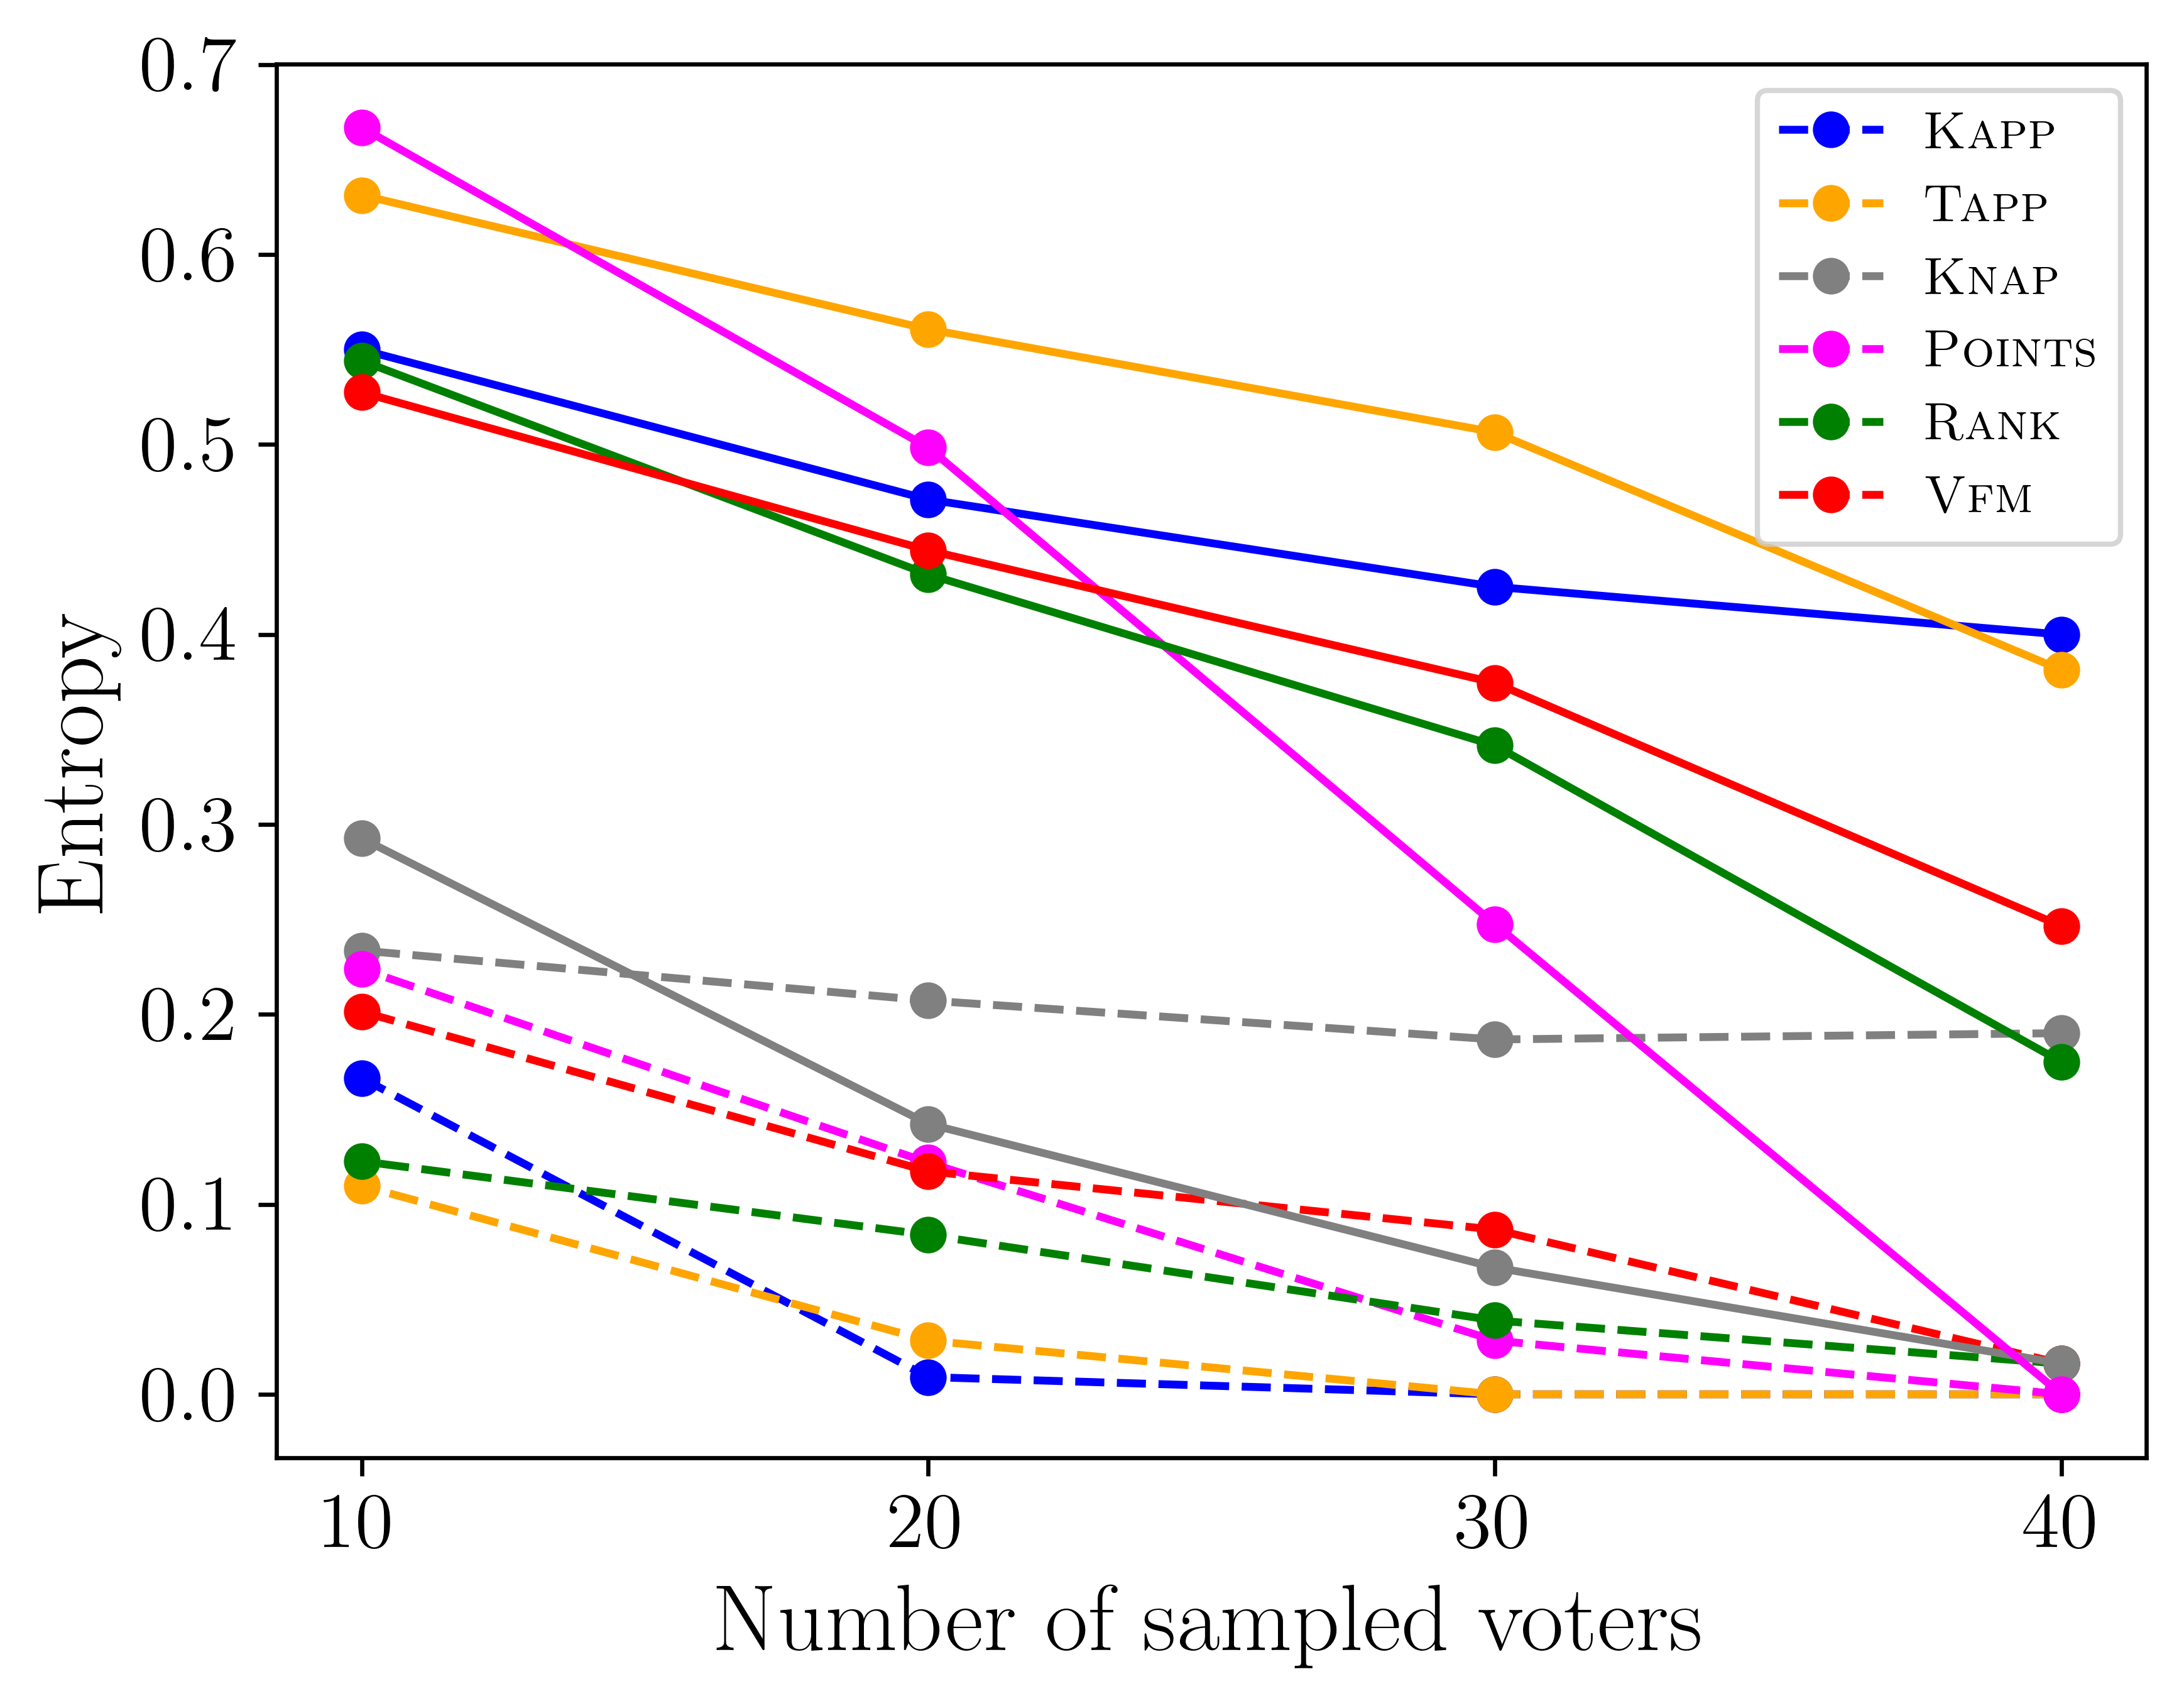
\includegraphics[width=7.5cm]{experiment/entropy_small_a.png}
\caption{Entropy for each input format under  greedy aggregation  (solid lines) and \mes{} (dotted lines)  as the number of sampled voters changes. }\label{fig:entropy}
\end{center}
\vspace{-3mm}
\end{figure}

\subsection{Social Welfare}
An obstacle to comparing outcomes based on social welfare is participants are assigned only one format, so there is no common basis of comparison when aggregating vote profiles from different formats. To address this, we make the assumption that, since voters are randomly assigned to input formats, the distribution of voter preferences are the same across formats. As such, we can deduce voter valuation functions from the full vote profile in \emph{any} format and treat these aggregated values as a proxy for the welfare of all voters, regardless which format they used.\footnote{ We caution that this is at best a very coarse evaluation, since assuming a value based on  a vote in any of the formats requires very strong assumptions. %However, it does allow for some form of comparison on the basis of welfare.
} % (while not a perfect metric, it let us get a sense on the quality of the outcomes welfare wise).  
%In order to compare the two methods, we will use two types of evaluations. First, the outcomes from the aggregation will be compared by the social welfare it achieve for the voters. Second, their stability will be tested, i.e. how well the method can represent the population given only part of it votes.

We report in Figure~\ref{fig:welfare} the   social welfare (averaged over the four elections) as measured when treating the full profile of \points{} or \knap{} voters as representative.  % Of course, these are only proxies for the true social welfare of the outcome and we are

%Starting with welfare, we will first notice that the true utility the voters get from the projects is unknown. Thus, we will use their reported preference and calculate utility. This mean that for each outcome (from all input formats) we can calculate the social welfare according to 6 different reported votes (one for each input format). 

Neither aggregation method strictly outperforms the other. However, we observe that, when using greedy aggregation, the choice of input format can have a large effect on welfare. This is seen most clearly when using \knap-voters to compute welfare. Unsurprisingly, \mes{} is less sensitive to  the choice of input format and   achieves very similar welfare across input formats.
Results when using the other formats to measure welfare are less extreme than the results shown here and may be found in Appendix~\ref{app:aggregation}.

%%%%%%%%%%%%%%%%%%%%%%%%%%%%%%%%%%%%%%%%%%%%%%%%%%%%%%%%%%%%%%%%%%%%%%%%%

\section{Discussion}

These results highlight practical insights  for the design of real participatory budgeting elections. 
When choosing an input format, we find no reason to deviate from the current standard practice of  using \kapp{} voting: Voters find the format easy to understand, easy to  use, and believe it allows them to express their preferences accurately. 

Greedy aggregation is used almost universally,  however, our experiments find that \mes{} has  two  big advantages over greedy aggregation.  First,  the outcomes are largely stable and unchanged when only a subset of the population participates. In light of low levels of real-world participation, we believe this is a particularly attractive property. Second, \mes{} appears to be robust to the choice of input format, in other words, it affords the city officials responsible for administering the participatory budgeting election a great deal of freedom to choose an input format which meets whatever secondary objectives are deemed to be important. % means that it allows officials a large degree of freedom to choose an input format which suits their objectives

One argument that remains in favour of greedy aggregation is its transparency: it is arguably easier to explain to voters than \mes{}. If greedy aggregation is used    and stability to partial participation is a primary concern, then \knap{} emerges as a fairly user-friendly format overall and a clear front-runner in terms of stability.

These recommendations should be taken in the context of the limitations of this study. First, the  behavior and preferences of participants recruited on Amazon Mechanical Turk may not be sufficiently similar to those of real voters.  Though we attempt to  ensure the findings are robust across the parameters of different elections by varying the number and type of projects, there is no mimicking the richness, variety and local idiosyncrasies of real-world instances. Similarly, real voter utilities likely exhibit complementarities and externalities  --- a far cry from our utility proxies. Second, it is possible that, despite our best efforts, the   voter experience   was affected by the interface design choices we made. 

\begin{figure}[!t]
\begin{center}
% 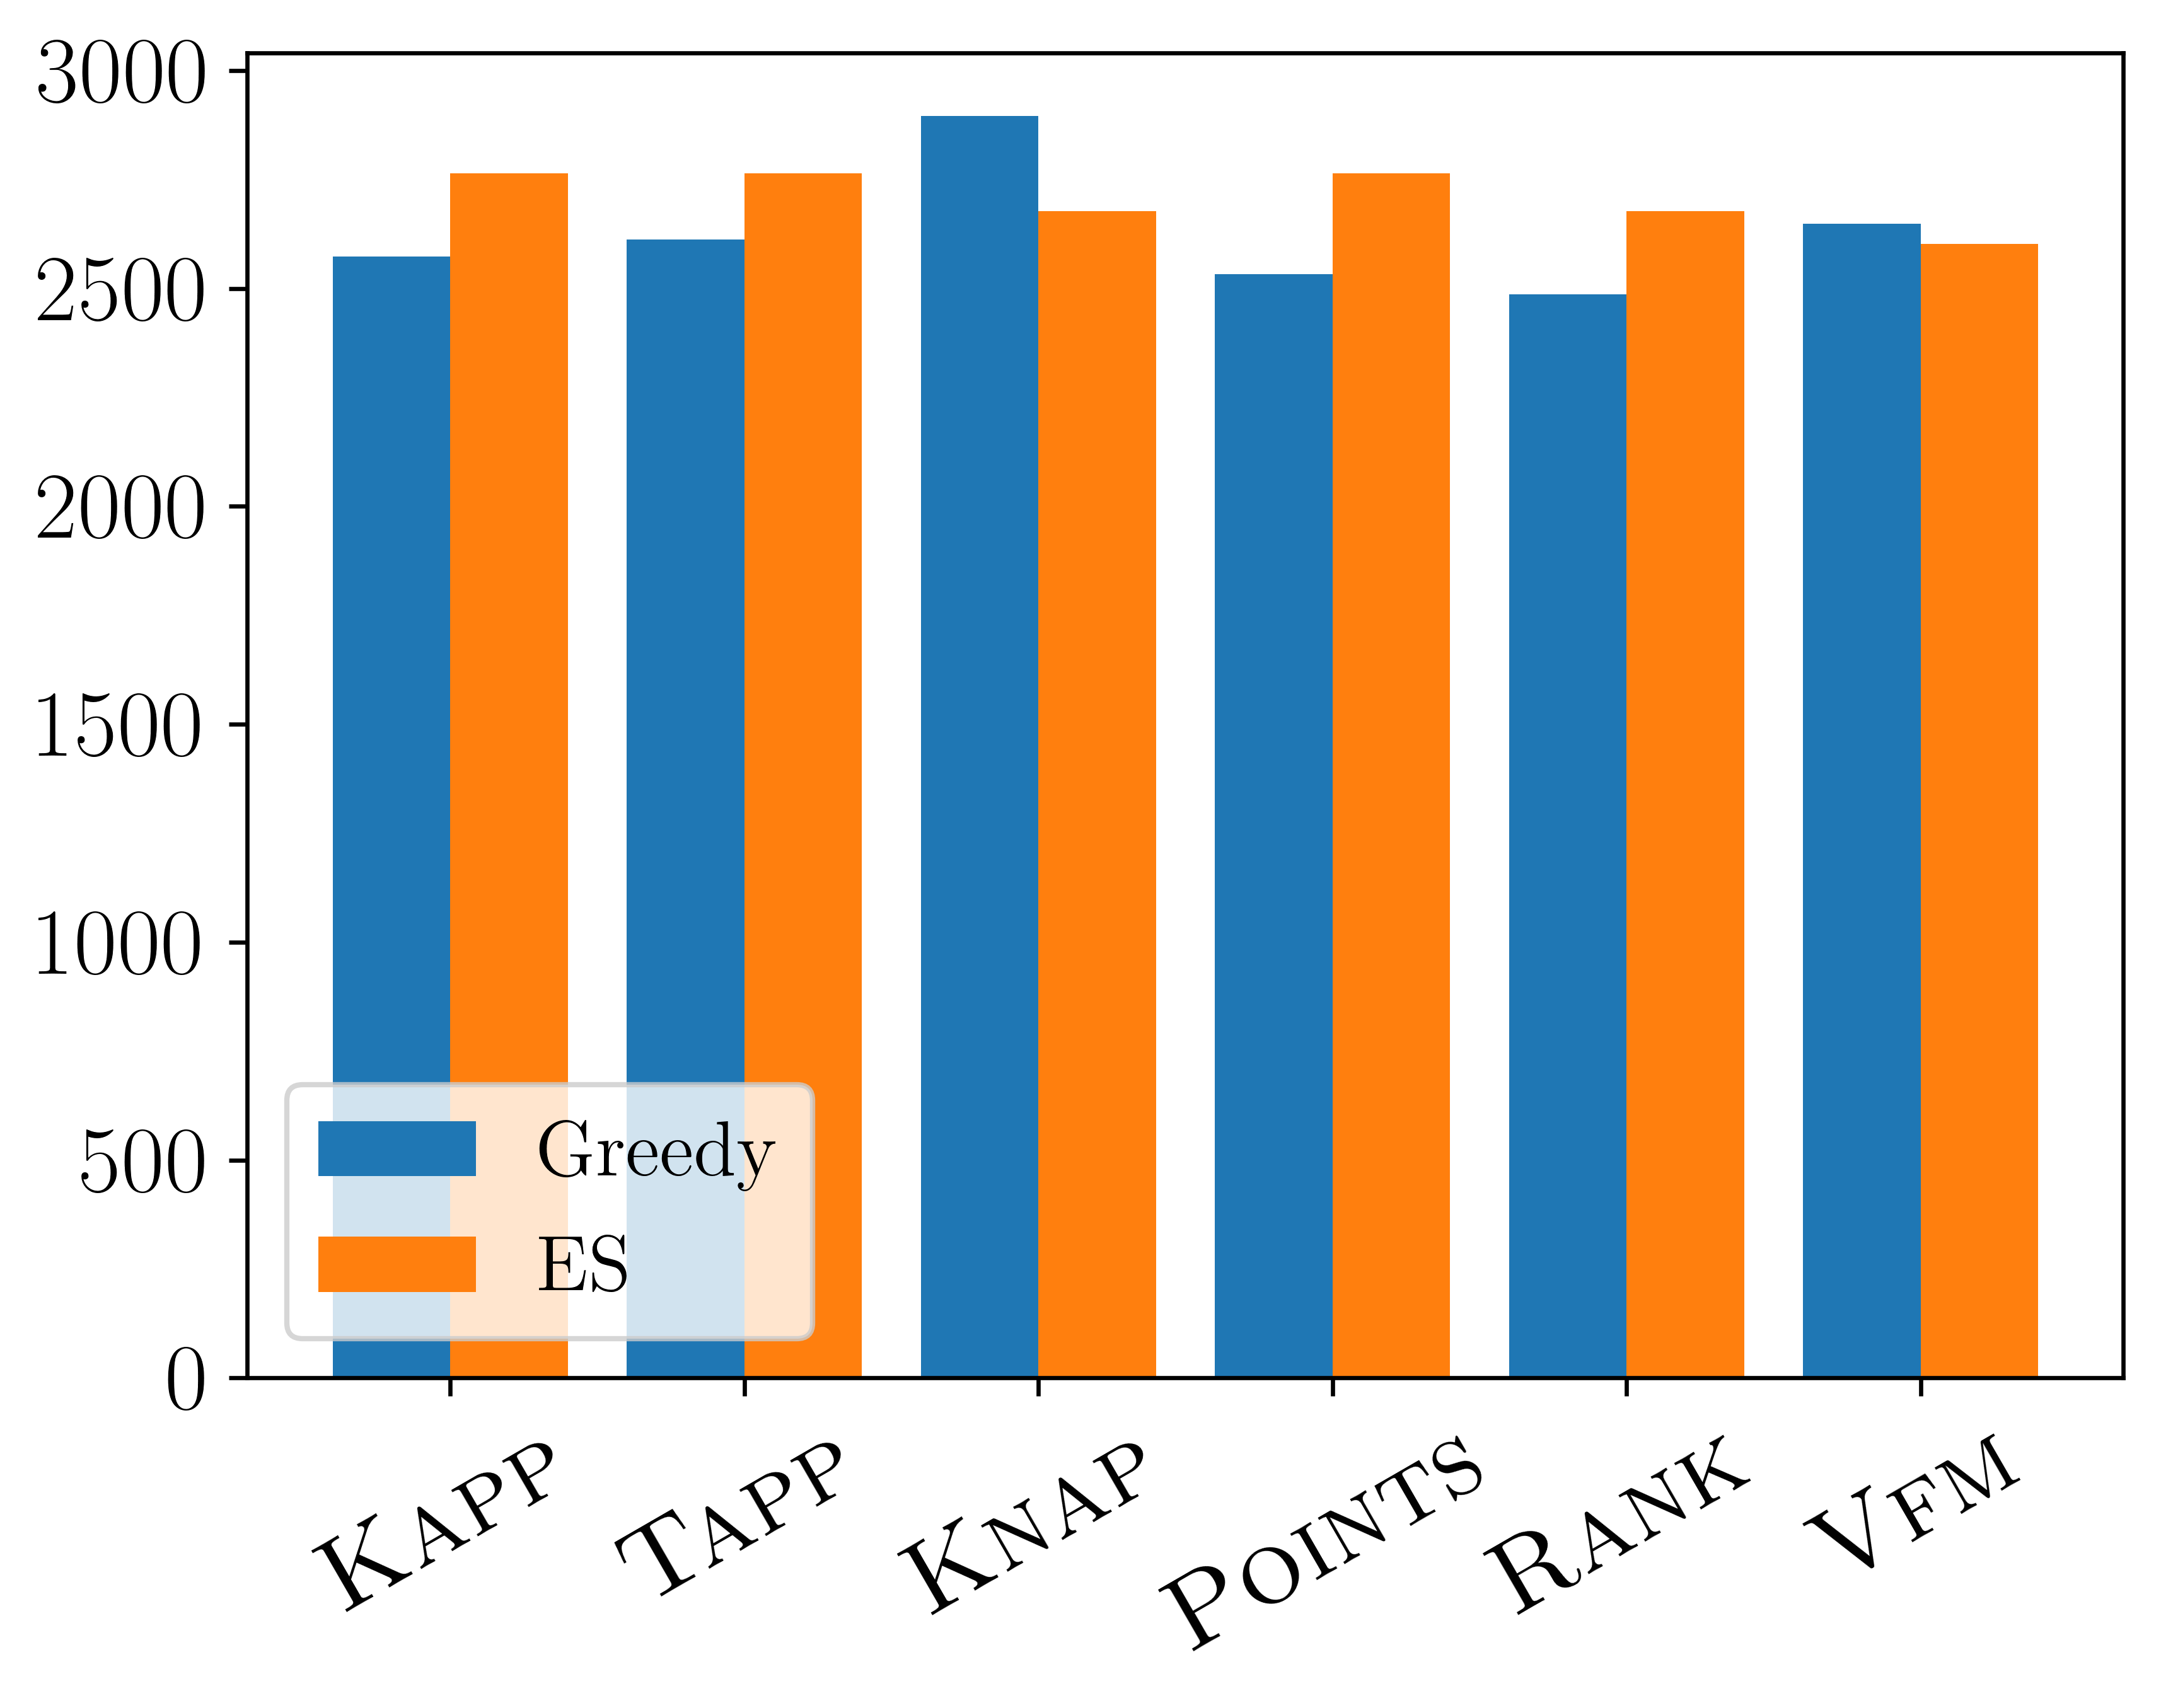
\includegraphics[trim={.8cm .5cm 1cm 1.3cm}, clip,width=4cm]{experiment/Utilities_welfare.png}
% 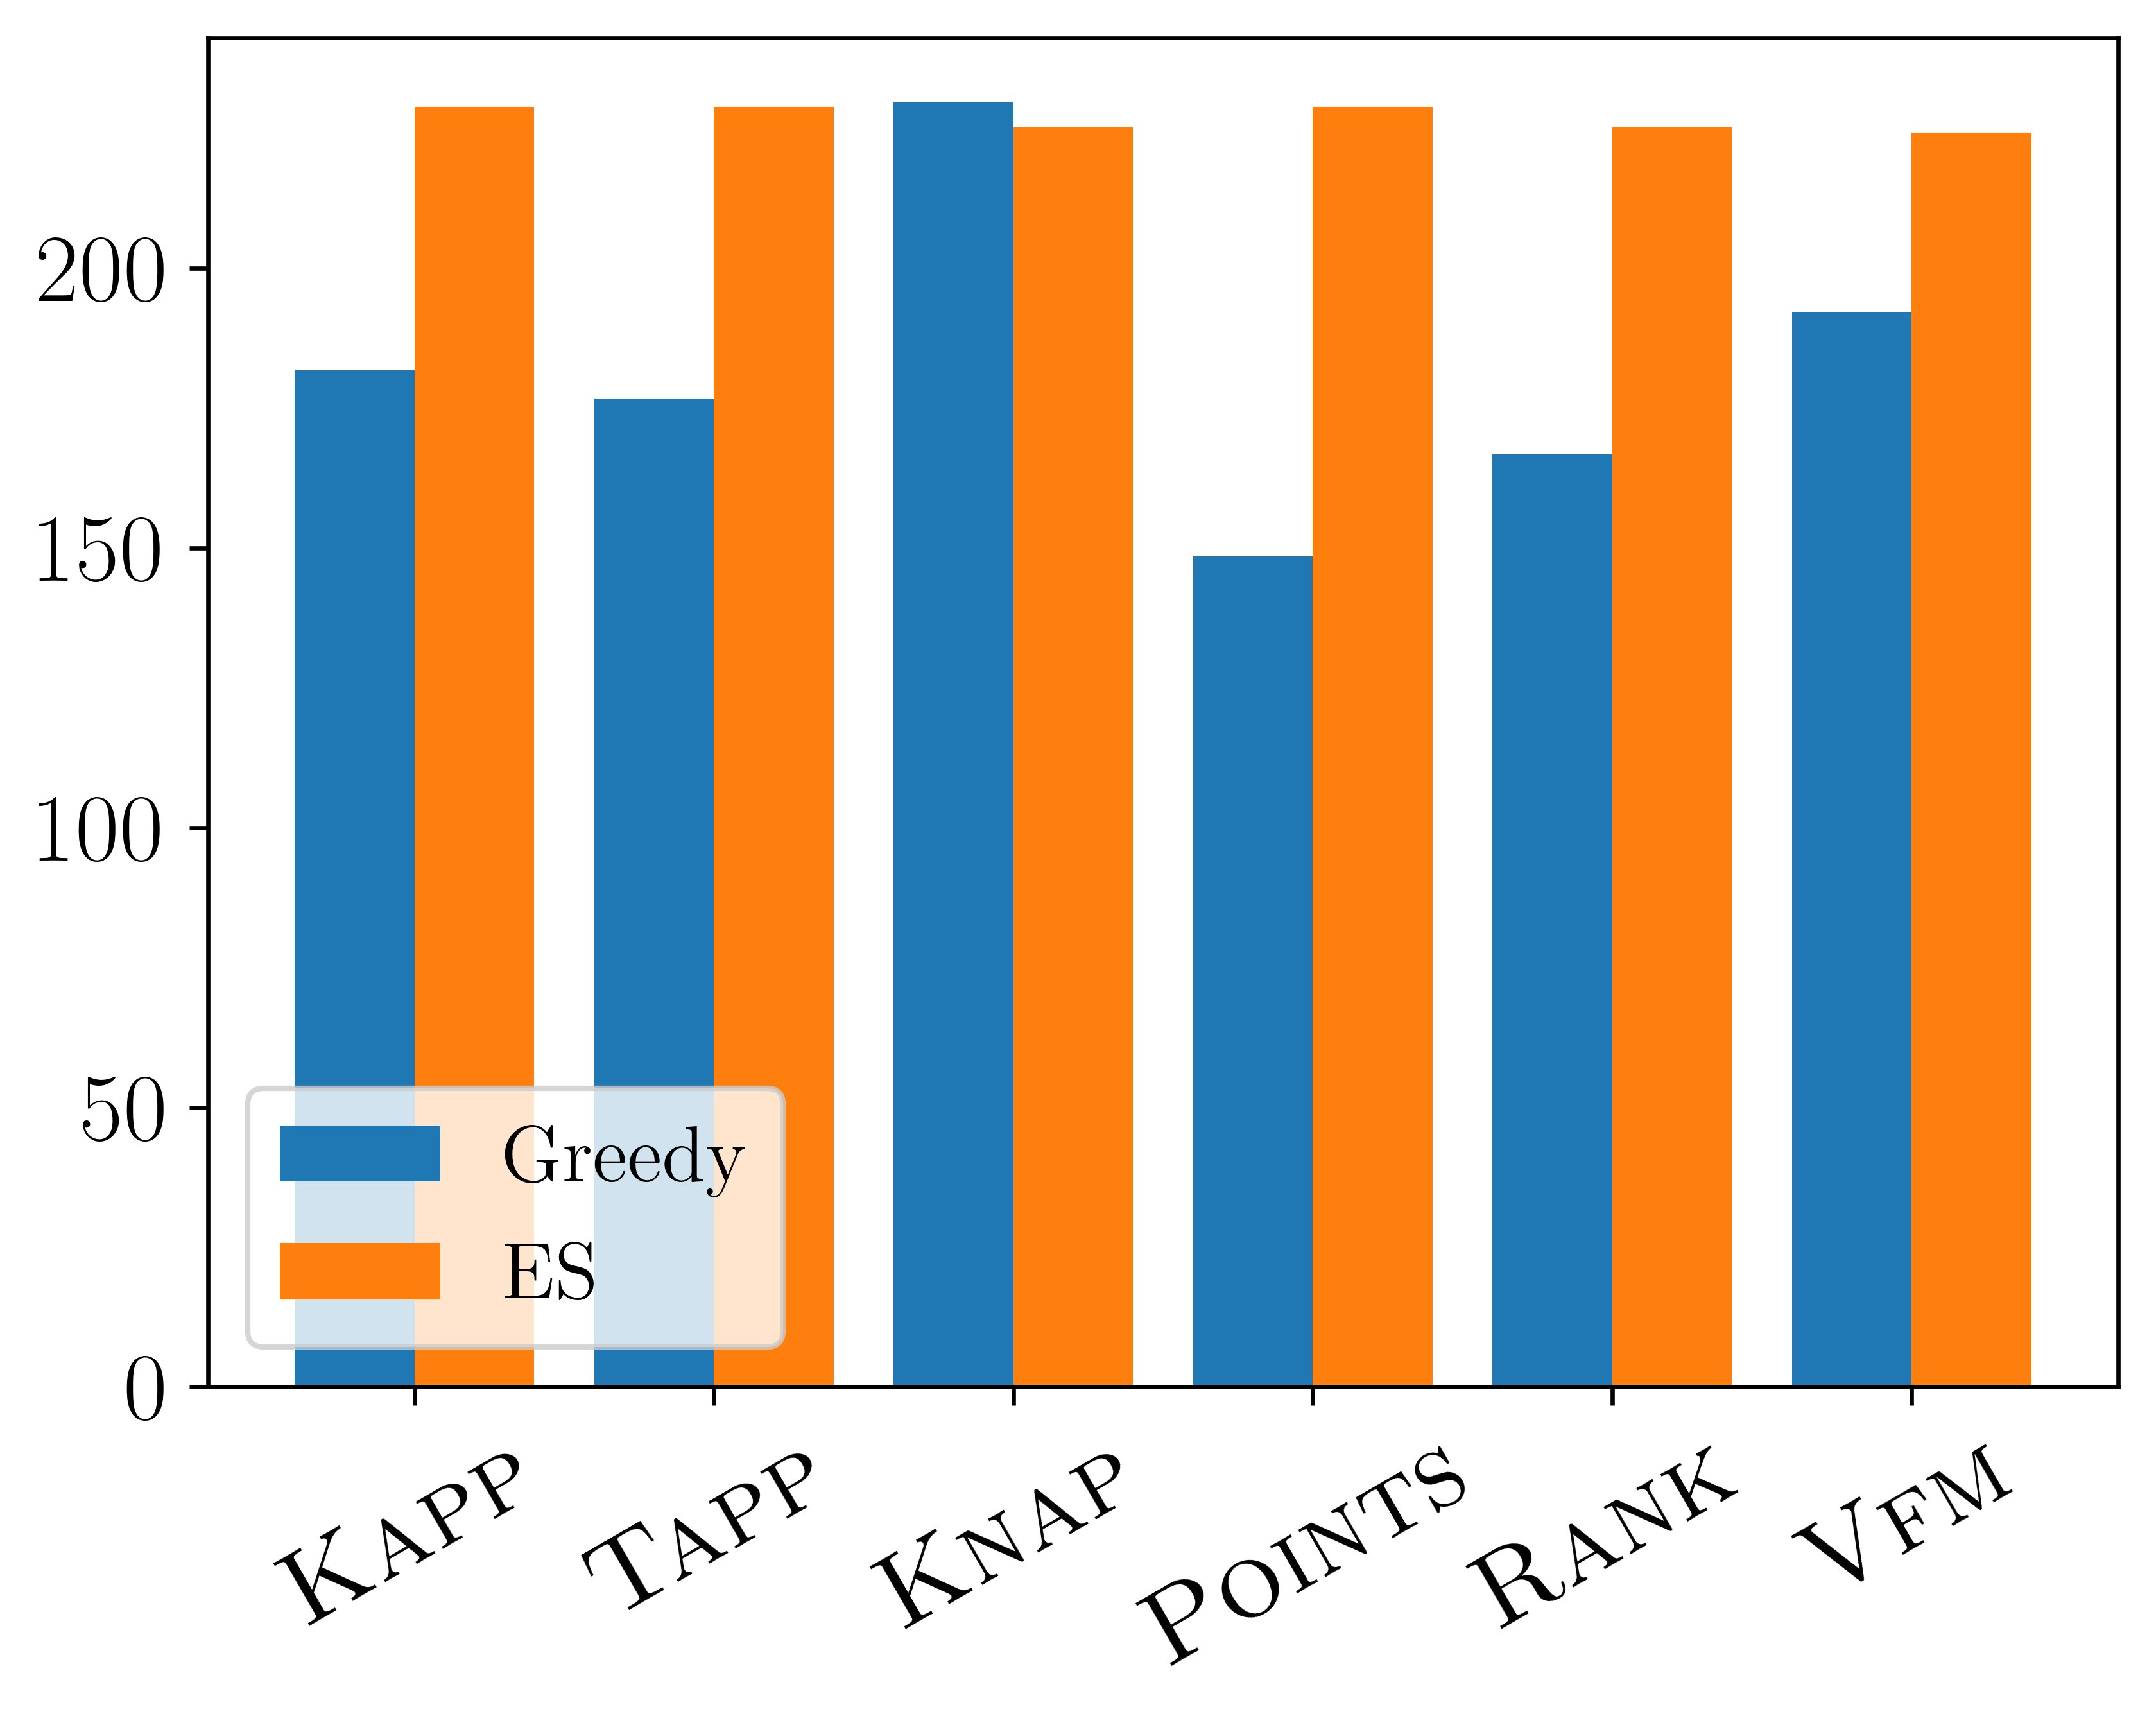
\includegraphics[trim={.8cm .5cm 1cm 1.3cm}, clip,width=4cm]{experiment/Knapsack_welfare.png}
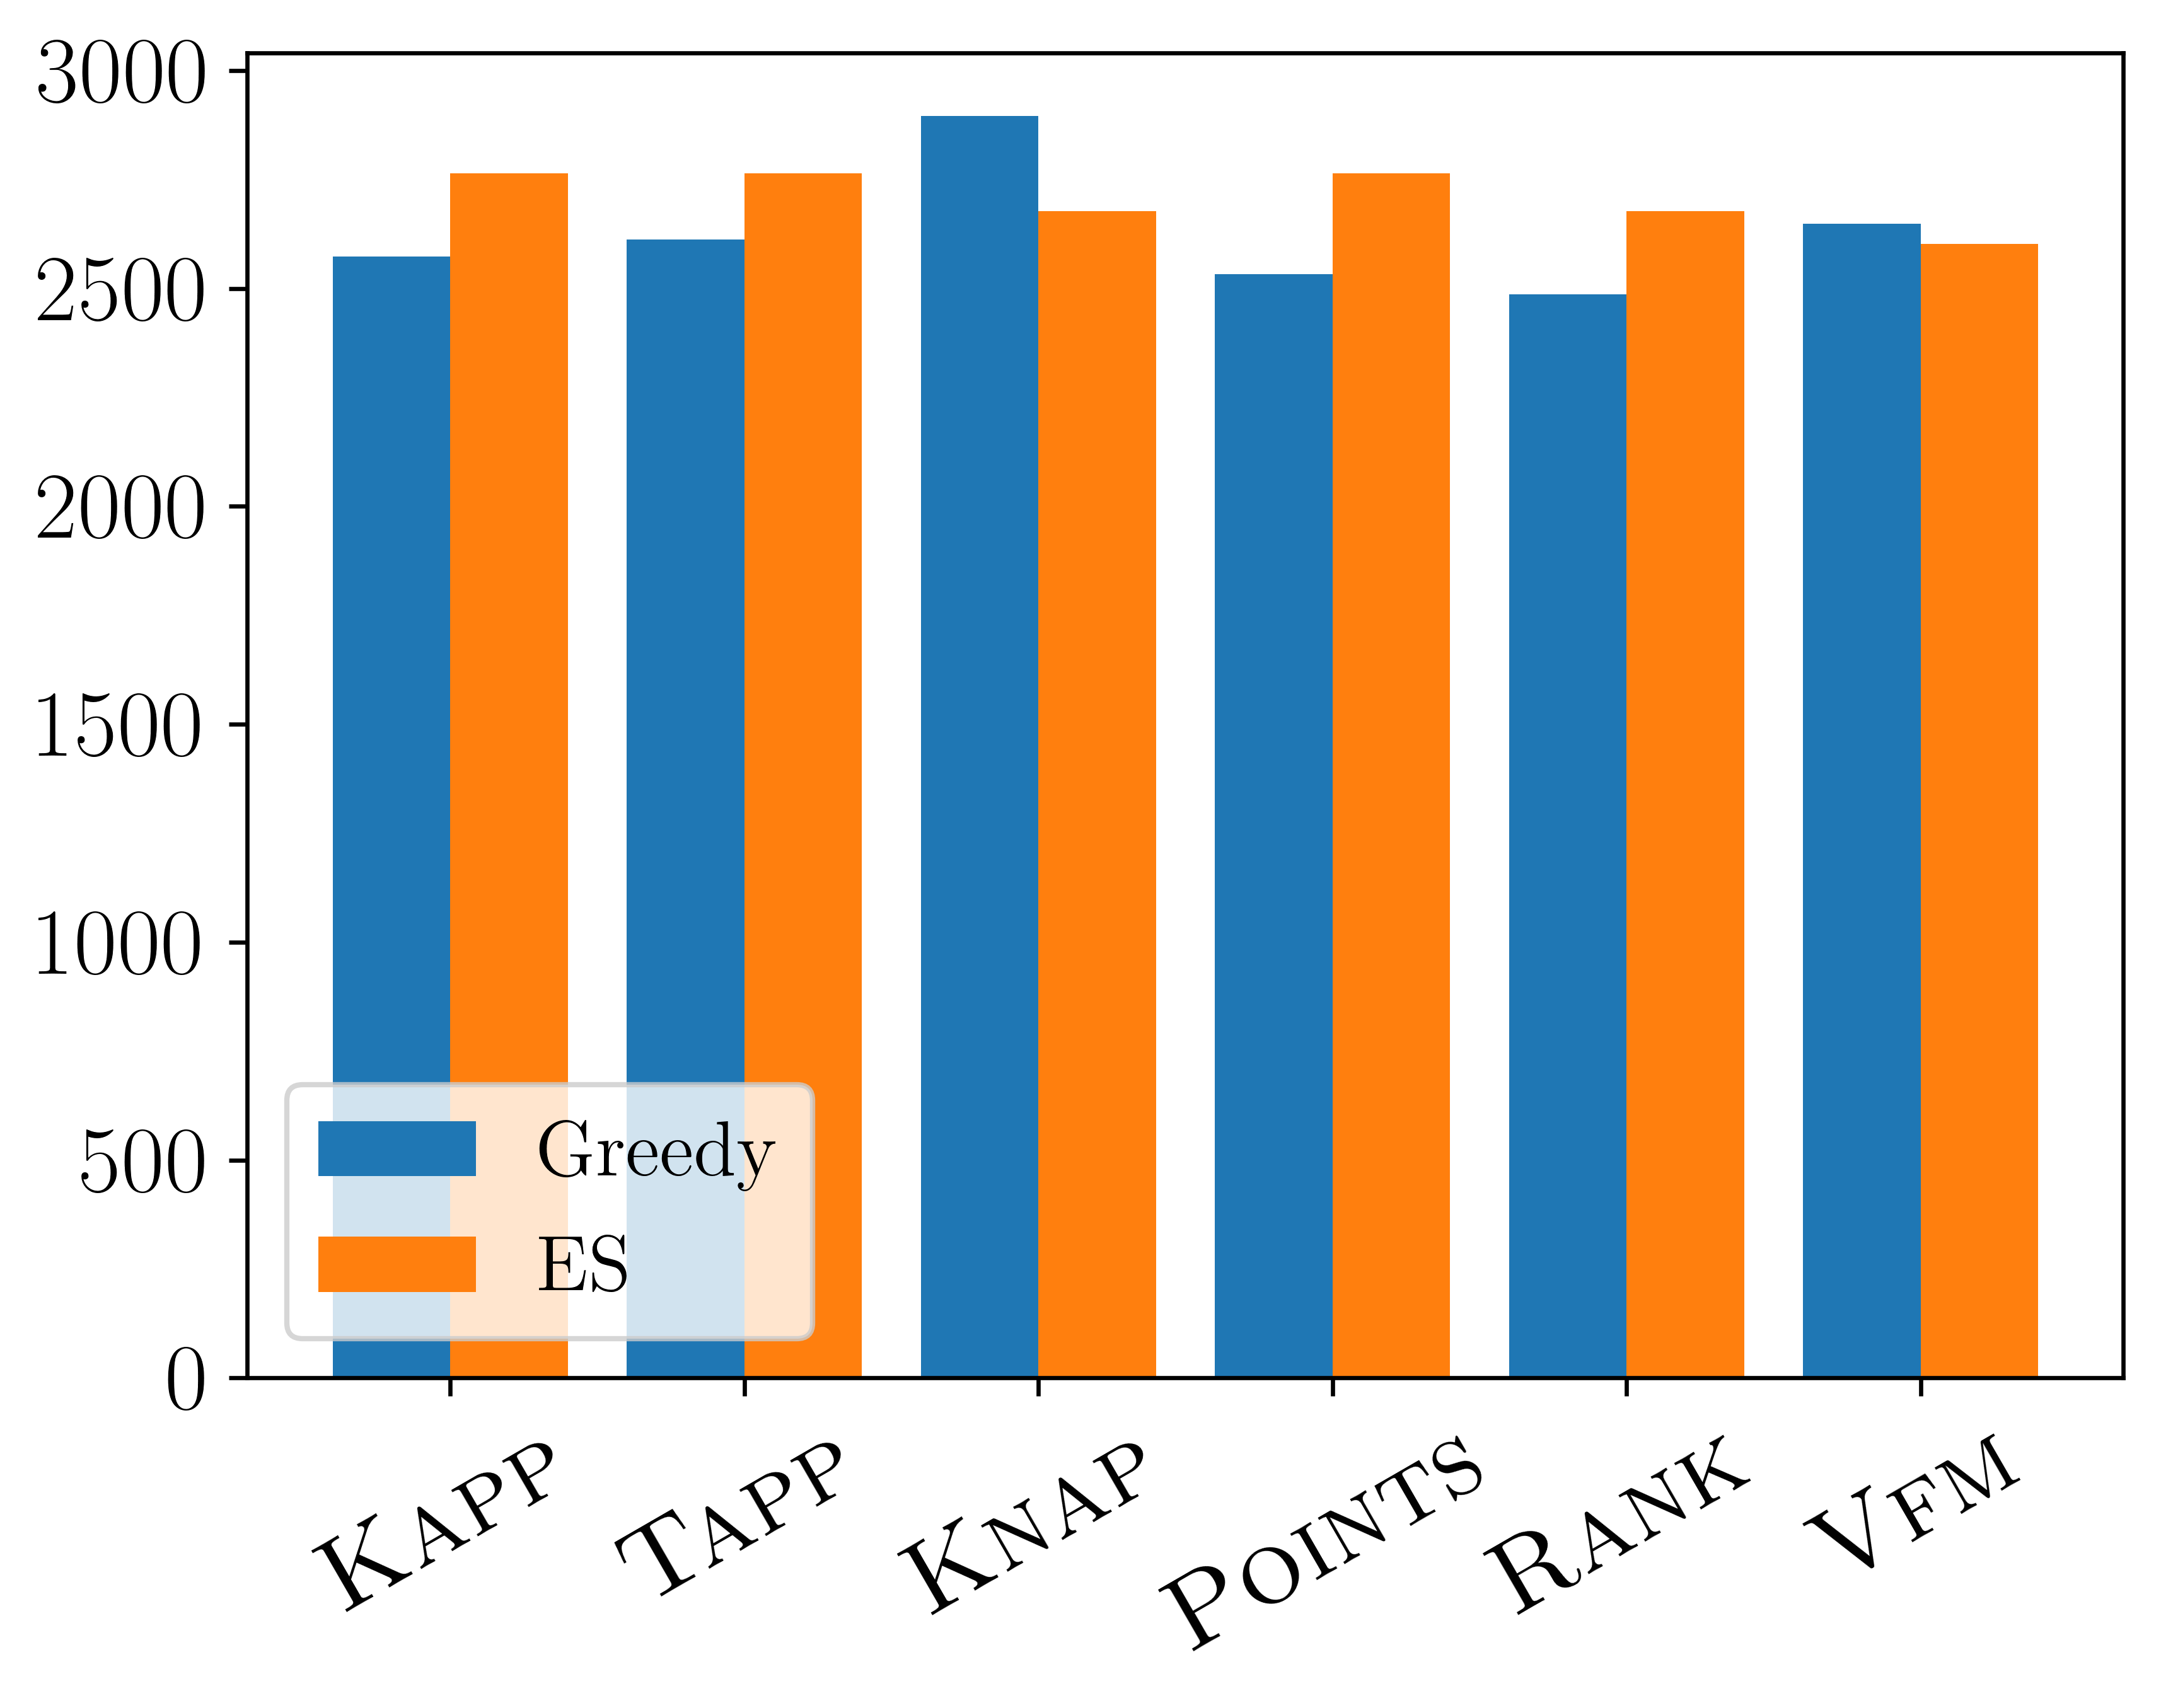
\includegraphics[width=6cm]{experiment/Utilities_welfare.png}
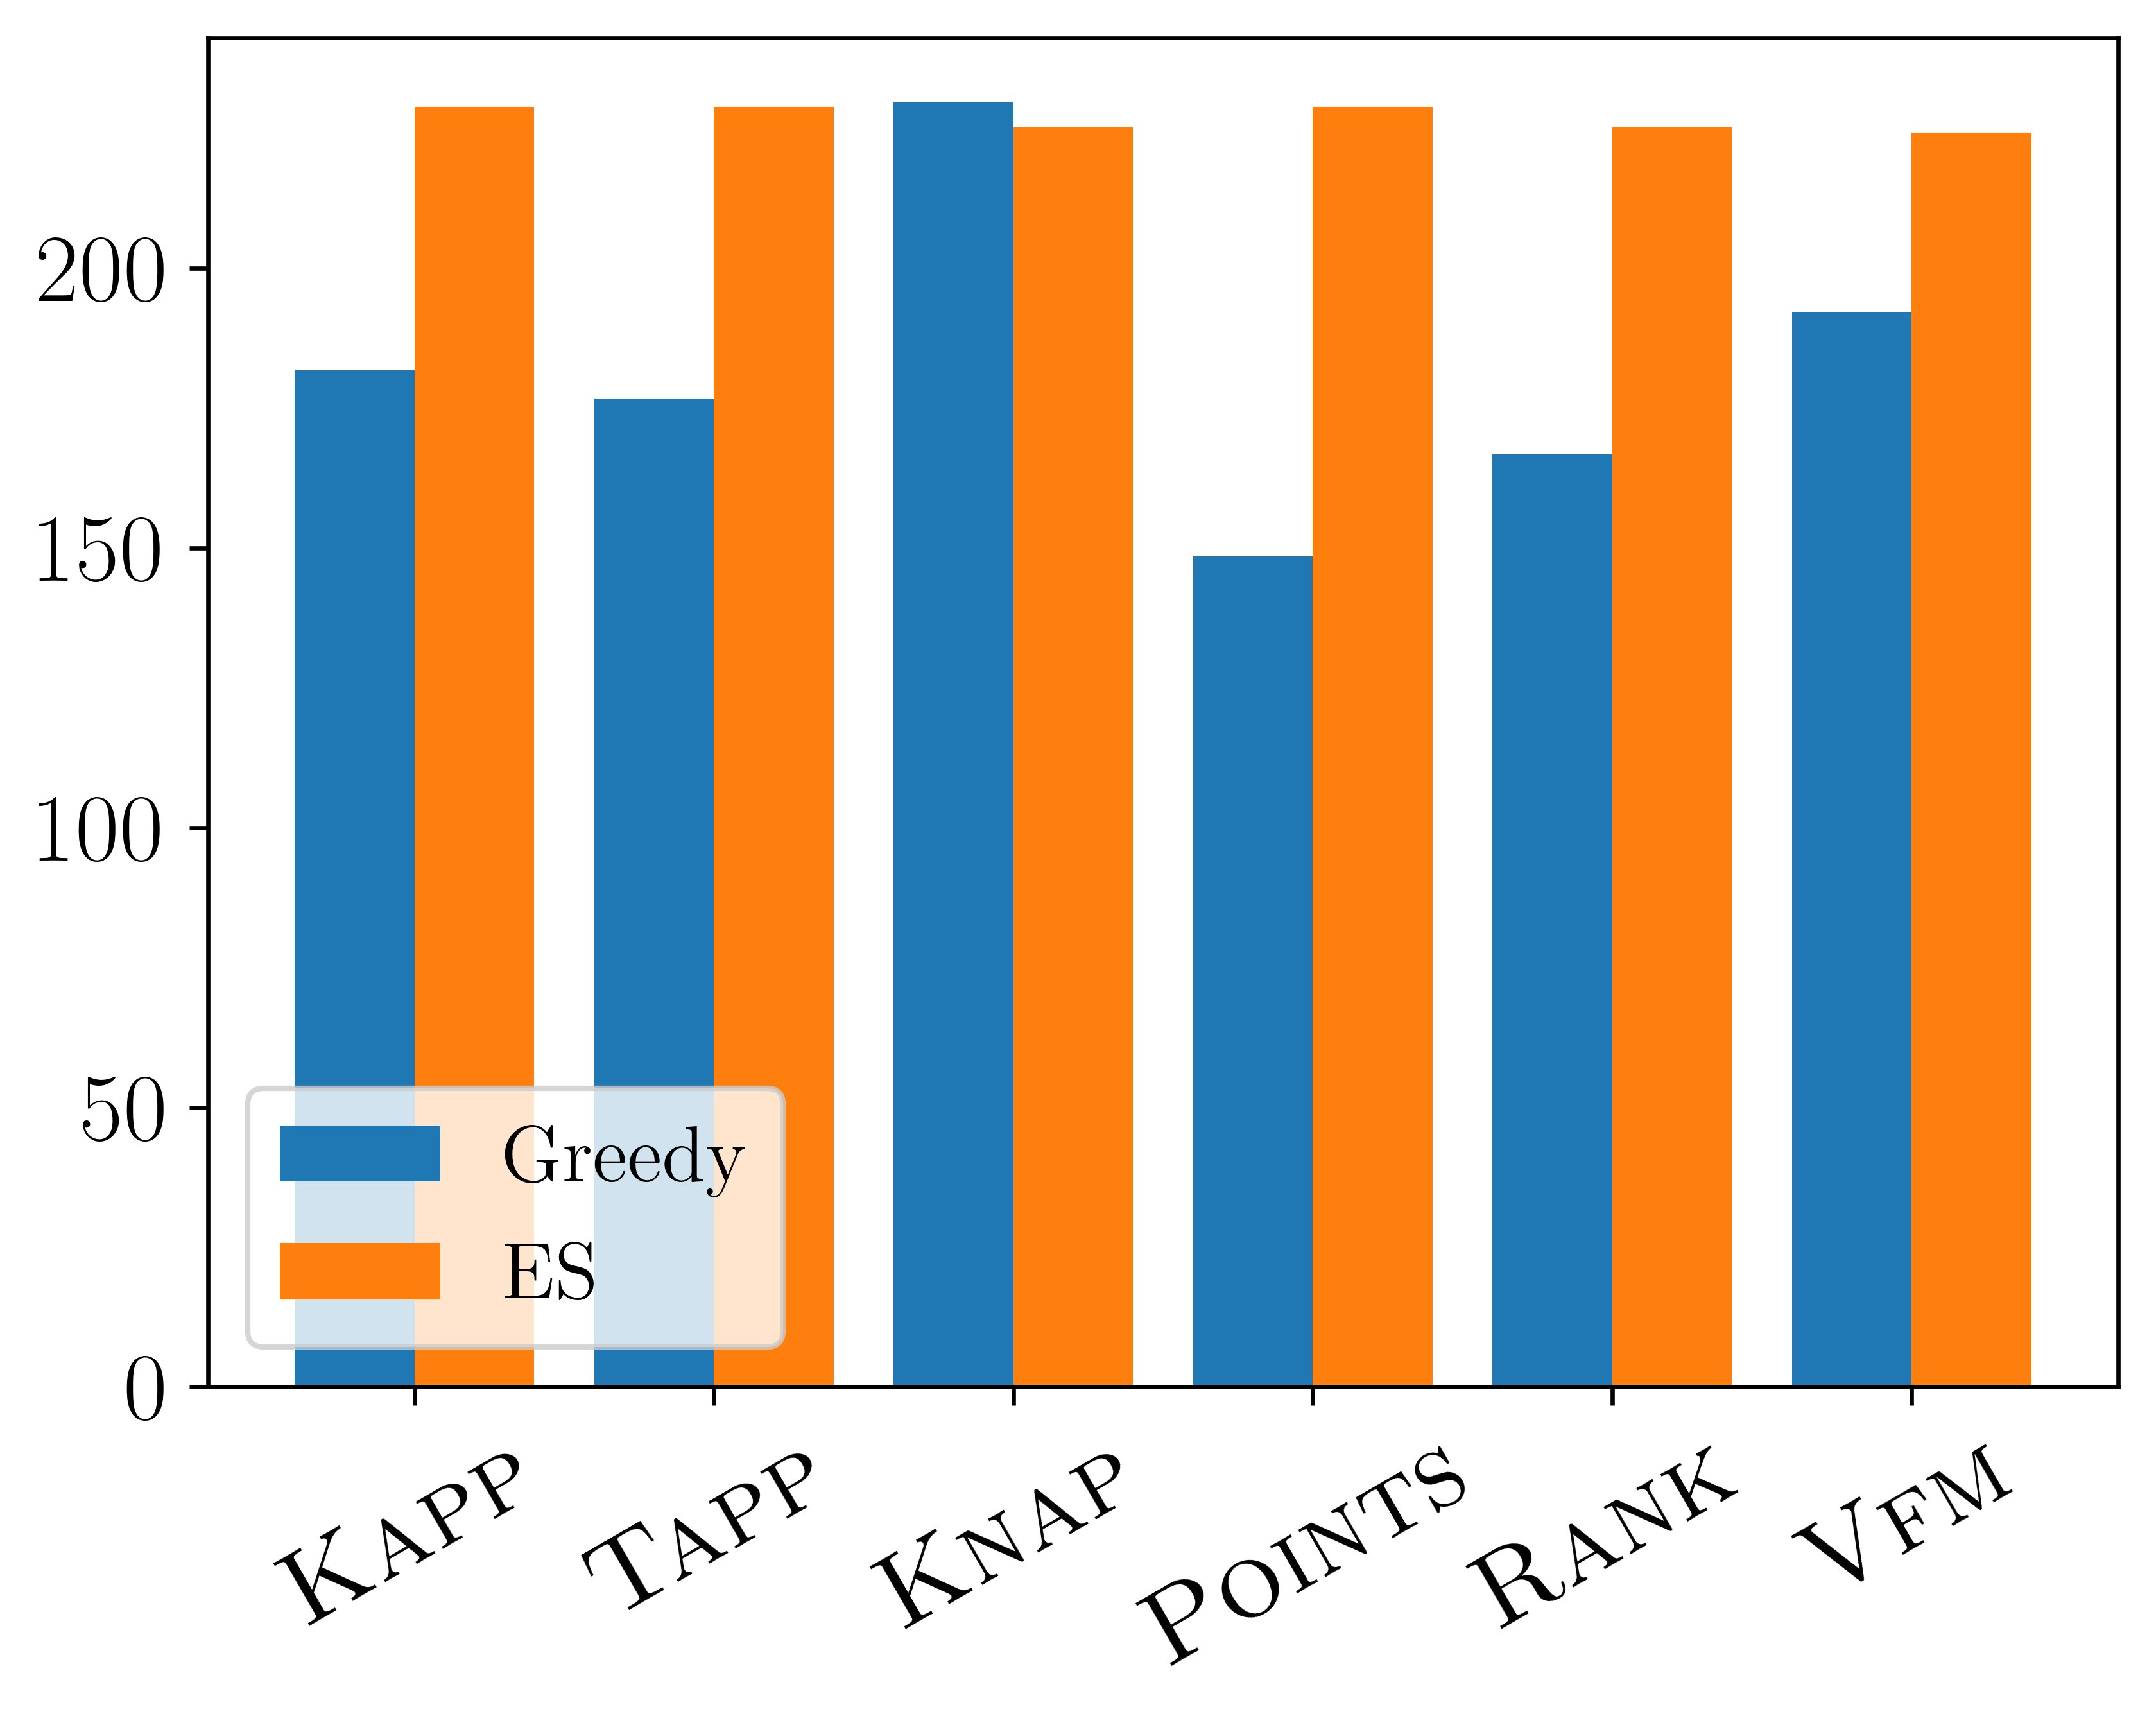
\includegraphics[width=6cm]{experiment/Knapsack_welfare.png}

\caption{Average social welfare (across elections) using the \points- (left) and \knap-voters (right) to compute welfare.
}\label{fig:welfare}
\end{center}\vspace{-5mm}
\end{figure}

We conclude with  two directions for future study. % and a challenge we believe is vital to overcome. % two   challenges  which   we believe are vital to overcome. % in closing the gap between practice and theory.  
When it comes to designing participatory budgeting elections, the proof, to a large extent, should be in the pudding.  %One may argue that 
%Perhaps a well-designed participatory budgeting election is one which yields an efficient and representative outcome.
One can imagine a  variant of the experiment presented in this paper in which votes from different PB designs are aggregated and voters are directly asked to compare different elections and outcomes on the transparency of the process, personal satisfaction, perceived fairness of the outcome, etc. 
Directly asking people their opinion about PB outcomes may yield new  insights   that can help inform design decisions while avoiding assumptions like  additive utilities. 

Democratic innovations live and die by the extent to which voters' voices are heard. But this requires representative participation. % , the voice of the people can only be heard if voters are willing to participate. 
As a fledgling part of the democratic process, participatory budgeting appears to be particularly susceptible to poor participation. It is important to understand how   design choices around voting formats and the transparency of aggregation rules affects the participation (now and in the future) of voters from a wide range of socio-economic backgrounds. Our stability experiments are a step in this direction but assume participation is uniform across the population, which is unlikely to be the case in reality. 

%%%%%%%%%%%%%%%%%%%%%%%%%%%%%%%%%%%%%%%%%%%%%%%%%%%%%%%%%%%%%%%%%%%%%%%%%

\section{Acknowledgments}
Nisarg Shah provided instrumental help and advice with all aspects of this research. Ariel Procaccia contributed to an earlier version of this paper. Thanks to Boaz Avami for programming assistance with the study. Roy Fairstein was funded in part by European Union’s Horizon 2020 WeNet project, under grant agreement 823783. 

%%%%%%%%%%%%%%%%%%%%%%%%%%%%%%%%%%%%%%%%%%%%%%%%%%%%%%%%%%%%%%%%%%%%%%%%%

% References
\bibliographystyle{plainnat}
\bibliography{ref.bib}
%%%%%%%%%%%%%%%%%%%%%%%%%%%%%%%%%%%%%%%%%%%%%%%%%%%%%%%%%%%%%%%%%%%%%%%%%

% At the very end of the paper, please include your contact details:

\begin{contact}
Roy Fairstein\\
Ben-Gurion University of the Negev\\
Beersheba, Israel\\
\email{royfa@post.bgu.ac.il}
\end{contact}

\begin{contact}
Gerdus Benad\`e\\
Boston University \\
Boston, USA\\
\email{benade@bu.edu}
\end{contact}

\begin{contact}
Kobi Gal\\
Ben-Gurion University of the Negev\\
Beersheba, Israel\\
\email{kobig@bgu.ac.il}
\end{contact}

%%%%%%%%%%%%%%%%%%%%%%%%%%%%%%%%%%%%%%%%%%%%%%%%%%%%%%%%%%%%%%%%%%%%%%%%%

\clearpage
\appendix

%%%%%%%%%%%%%%%%%%%%%%%%%%%%%%%%%%%%5

\section{Interface For Voting}\label{app:interfaces}
Figure~\ref{fig:kapp_inter}-\ref{fig:util_inter} shows   the interface for each of the input formats.

\begin{figure*}[ht!]
     \centering
          \begin{subfigure}[b]{0.45\textwidth}
         \centering
       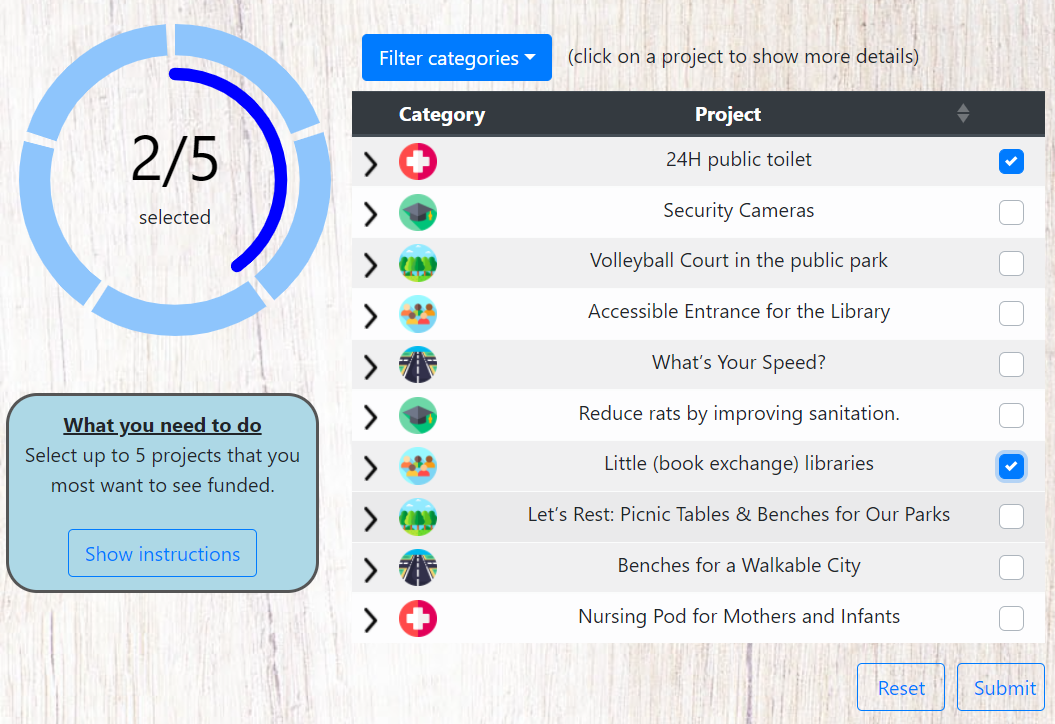
\includegraphics[width=6cm]{experiment/k approval.PNG}
\caption{\kapp{} user interface.
}\label{fig:kapp_inter}
     \end{subfigure}\hfill
     \begin{subfigure}[b]{0.45\textwidth}
         \centering
         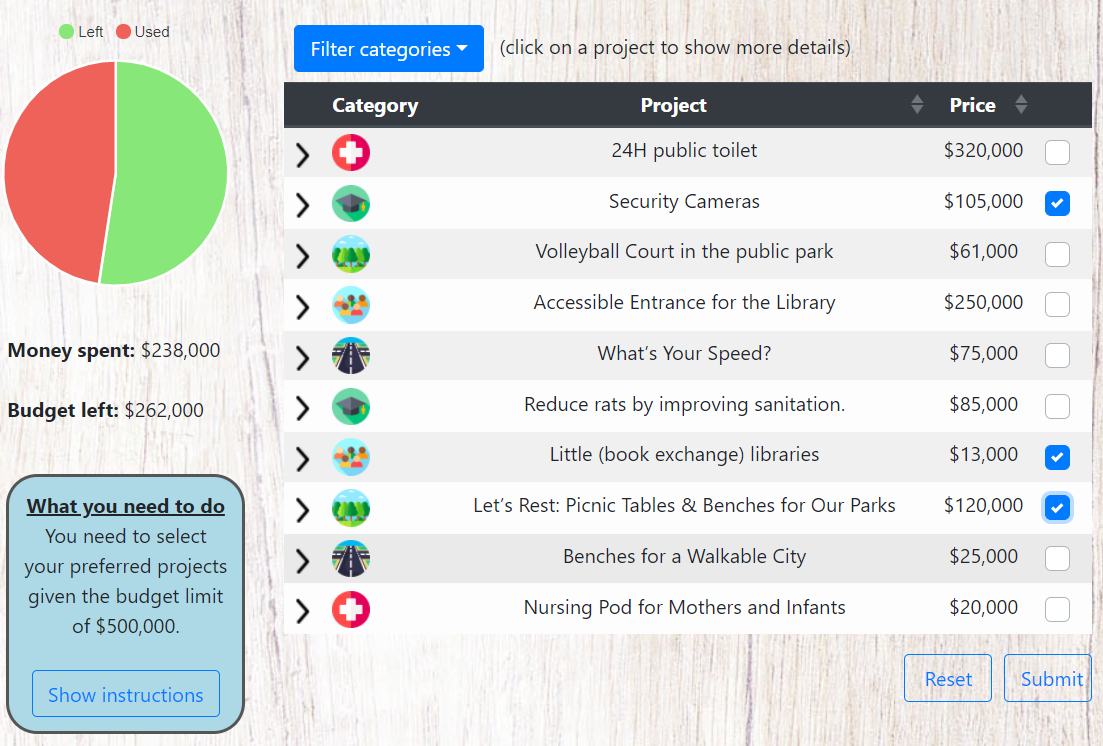
\includegraphics[width=6cm]{experiment/knapsack.PNG}
\caption{\knap{}  user interface.
}\label{fig:knap_welfare_app}
     \end{subfigure}
     \hfill
     \begin{subfigure}[b]{0.45\textwidth}
         \centering
         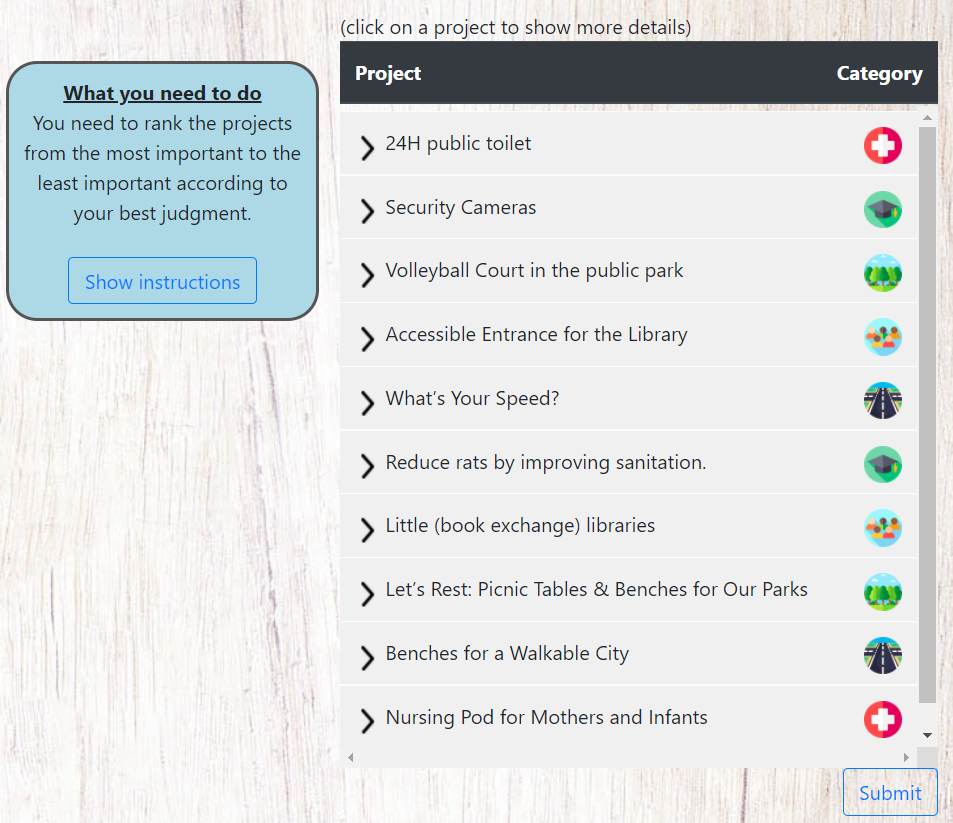
\includegraphics[width=6cm]{experiment/ranking.PNG}
\caption{\rank{} user interface.
}\label{fig:rank_inter}
     \end{subfigure}
     \hfill
     \begin{subfigure}[b]{0.45\textwidth}
         \centering
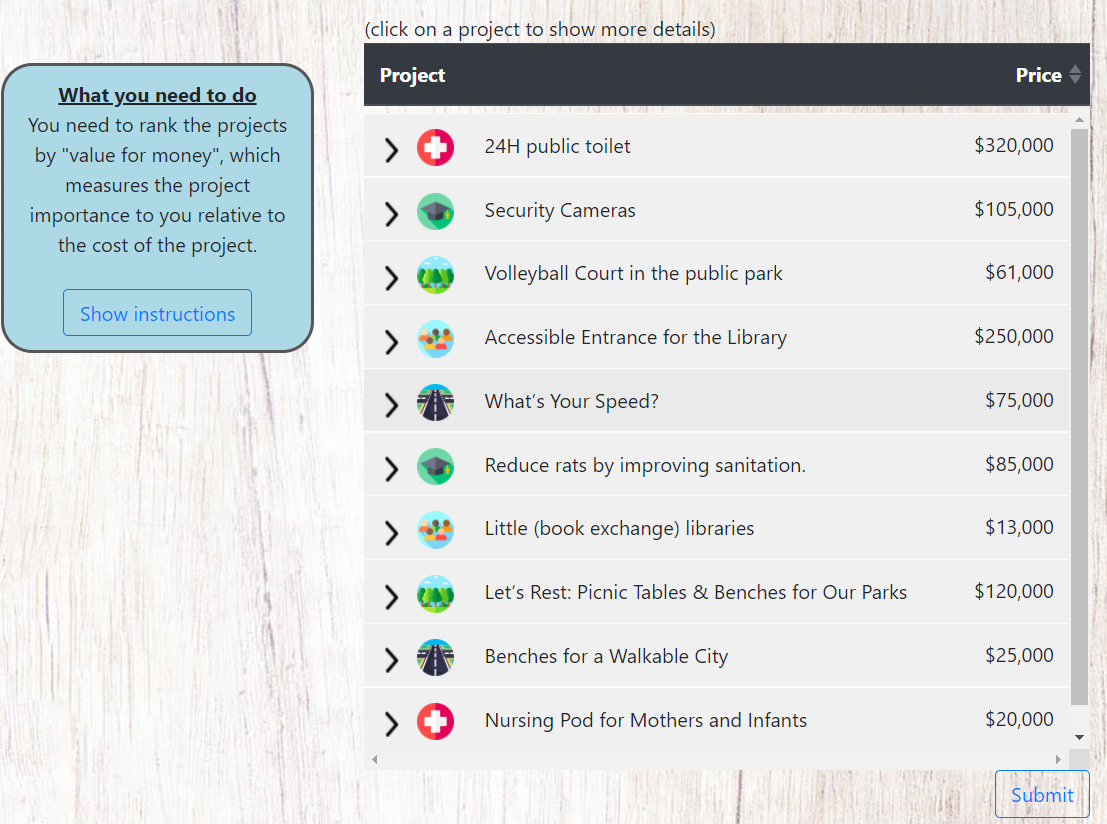
\includegraphics[width=6cm]{experiment/ranking by cost.PNG}
\caption{\vfm{} user interface.
}\label{fig:vfm_inter}
     \end{subfigure}
     \begin{subfigure}[b]{0.45\textwidth}
         \centering
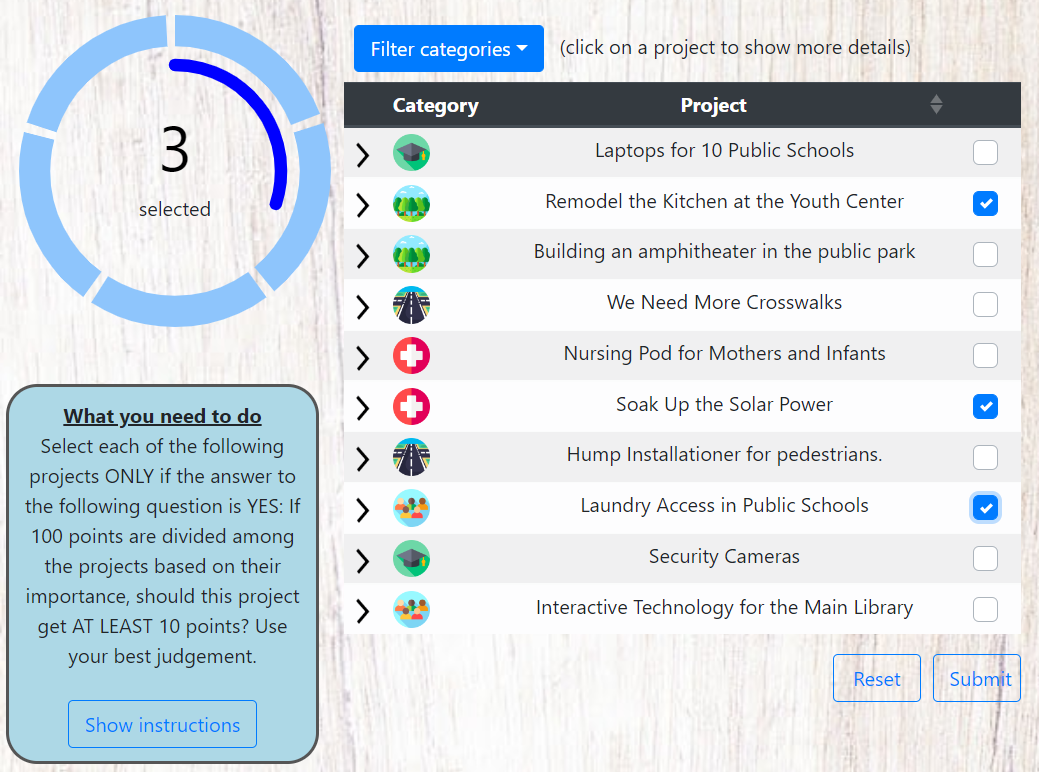
\includegraphics[width=6cm]{experiment/threshold approval.PNG}
\caption{\tapp{} user interface.
}\label{fig:tapp_inter}
     \end{subfigure}
     \hfill
     \begin{subfigure}[b]{0.45\textwidth}
         \centering
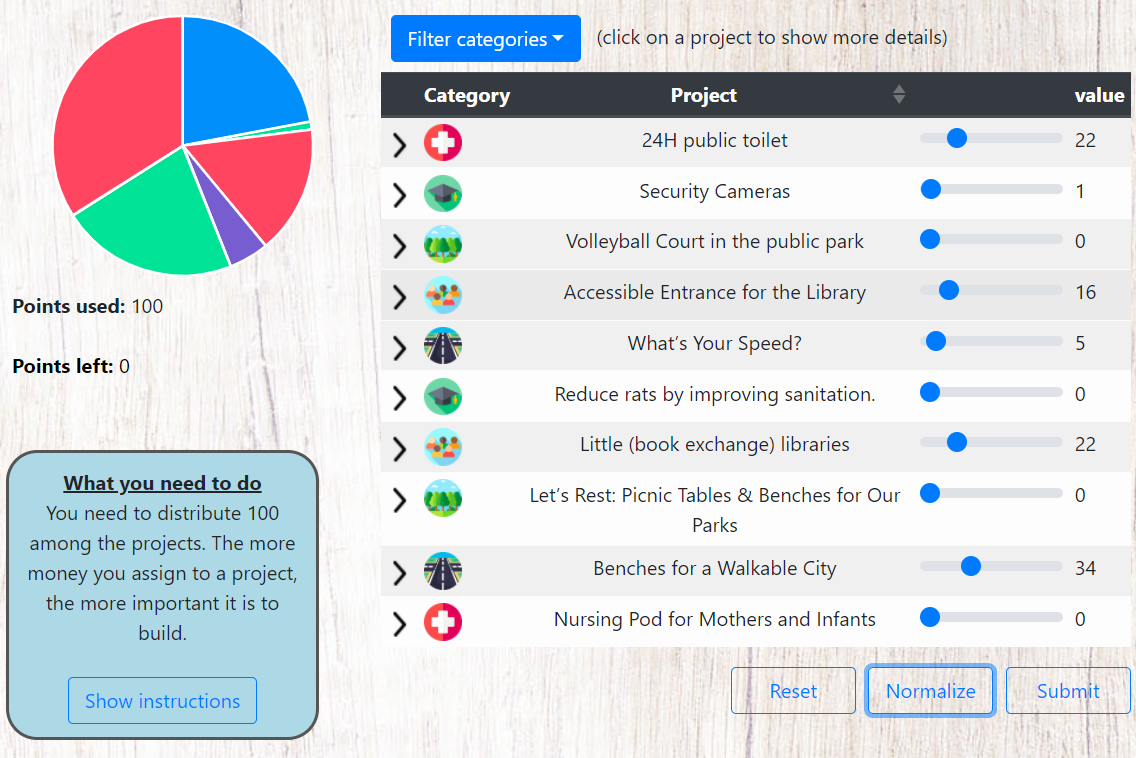
\includegraphics[width=6cm]{experiment/utilities.PNG}
\caption{\points{} user interface.
}\label{fig:util_inter}
     \end{subfigure}
     

        \caption{Input formats interface.}
        \label{fig:all_interfaces}
\end{figure*}


%%%%%%%%%%%%%%%%%%%%%%%%%%%%%%%%%%%%%%%%%%%
\section{Experiment Configurations}\label{app:elections}

In the experiments each participant encountered one of six input formats and one of 4 possible elections, each with different set of projects, either 10 projects or 20, such that each project belong to one of 5 categories:

\begin{itemize}
    \item Culture and community.
    \item Streets, Sidewalks and Transit.
    \item Environment, public health and safety.
    \item Facilities, parks and recreation.
    \item Education.
\end{itemize}

Tables~\ref{tab:first_elc}-\ref{tab:fourth_elc} show the four different elections the participants might encounter in the experiment, a short description, and to which category it belongs. The given coordinates are for 100x100 map, certain projects include several coordinates.


%%%%%%%%%%%% SMALL A election %%%%%%%%%%%%%%%%%%%%
\begin{longtable}[ht!]{|p{2cm}|p{6cm}|p{3cm}|p{1cm}|p{2.5cm}|}
  % \begin{center}
  %   \begin{tabular}
    \hline
    \textbf{Project} & \textbf{Description} & \textbf{Category} & \textbf{Price} & \textbf{Coordinates}\\
    \hline
    Computers for the community learning center & Funding 20 laptops including mice and keyboards, giving students a place to study & Culture and community &  27K & (55,55)\\
    \hline
    Laundry Access in Public Schools & Renovate a space in a Cambridge Public School and install washers and dryers for students who do not have easy access to laundry services at home, to use for their clothing and necessities & Culture and community & 50K & (25,45)\\
    \hline
    Real-Time Bus Arrival Monitors in bus stations & Real-time bus arrival monitors bus stops will inform travelers when the next bus will arrive, so they can adjust their plans if needed &  Streets, Sidewalks and Transit &  24K & (65,15) (35,85) (75,75)\\
    \hline
    Sheltered Bike Parking at the Main Library & The Main Library needs more bicycle parking. A glass pavilion, protecting bikes from the weather, landscaped with paths and trees, will be an attractive and functional addition to the library grounds & Streets, Sidewalks and Transit & 90K & (45,25)\\
    \hline
    24H public toilet & 24-hour access public toilet near Central Square & Environment, public health and safety & 320K & (70,35)\\
    \hline
    The Sustainable Energy Pilot & Install energy conversion devices on gym equipment and a rapid electric vehicle charging station & Environment, public health and safety & 90K & (10,25)\\
    \hline
    Dog Park & Building a dog park & Facilities, parks and recreation & 250K & (55,85)\\
    \hline
    Let’s Rest: Picnic Tables and Benches for Our Parks & Benches and picnic tables bring our community together. Installing new benches and picnic tables in up to 10 of our park will allow people of all ages and abilities to enjoy them for resting, talking, reading, people watching and being outdoors & Facilities, parks and recreation & 120K & (75,25) (90,55) (95,25)\\
    \hline
    Installing Lights at the school Basketball Court & Install lighting to extend safe playing hours for basketball courts. Increases safety for community members while expanding healthy alternatives for youth and access to public space & Education & 250K & (25,55)\\
    \hline
    Security Cameras & Install security cameras in public schools & Education & 105K & (35,10) (50,45) (40,60)\\
        
     \hline
    % \end{tabular}
  \caption{First small election (\textsc{Small-A})}\label{tab:first_elc}.
  % \end{center}
\end{longtable}

%%%%%%%%%%%% SMALL B election %%%%%%%%%%%%%%%%%%%%
% \clearpage
\begin{longtable}[ht!]{|p{2cm}|p{6cm}|p{3cm}|p{1cm}|p{2.5cm}|}
  % \begin{center}
    % \begin{tabular}
    \hline
    \textbf{Project} & \textbf{Description} & \textbf{Category} & \textbf{Price} & \textbf{Coordinates}\\
    \hline
    Interactive Technology for the Main Library & This project will fund an iPad lending kiosk and 16 iPads, as well as a permanent interactive screen in the Children’s Room of the Main Library & Culture and community & 60K & (5,5)\\
    \hline
    Laundry Access in Public Schools & Renovate a space in a Cambridge Public School and install washers and dryers for students who do not have easy access to laundry services at home, to use for their clothing and necessities & Culture and community & 50K & (90,75)\\
    \hline
    We Need More Crosswalks & To enhance pedestrian safety, this project will add a minimum of five new crosswalks to major streets & Streets, Sidewalks and Transit &  40K & (55,35) (35,25) (35,55)\\
    \hline
    Hump Installationer for pedestrians & Speed humps create a safer environment by helping slow traffic on streets that students and families cross frequently. When a car hits a pedestrian at a high rate of speed, the collision is more likely to result in a pedestrian fatality. Speed humps slow vehicles and give drivers increased response time and distance for stopping. This makes streets safer for pedestrians & Streets, Sidewalks and Transit & 66K & (75,65)\\
    \hline
    Nursing Pod for Mothers and Infants & Provide an attractive private space where working mothers and community members can breastfeed or pump during the work day & Environment, public health and safety & 20K & (55,85) (50,3) (20,90)\\
    \hline
    Soak Up the Solar Power & Free, clean, renewable energy! Let’s add solar panels to the Youth Center to reduce greenhouse gas emissions and save money on energy & Environment, public health and safety & 250K & (45,25)\\
    \hline
    Building an amphitheater in the public park & Build an amphitheater in the public park for outdoor performances, music, stories, and other cultural events that the whole community can enjoy & Facilities, parks and recreation & 350K & (70,20)\\
    \hline
    Remodel the Kitchen at the Youth Center & The kitchen area in the Youth Center is in dire need of renovating. Replace the stove, dishwasher, cabinets, and countertops in the Youth Center kitchen & Facilities, parks and recreation & 200K & (90,40)\\
    \hline
    Laptops for 10 Public Schools & Purchasing laptop carts for ten public schools & Education & 350K & (50,50)\\
    \hline
    Security Cameras & Install security cameras in public schools & Education & 105K & (20,50)\\
     \hline
    % \end{tabular}
  \caption{Second small election (\textsc{Small-B})}\label{tab:second_elc}.
  % \end{center}
\end{longtable}


%%%%%%%%%%%% LARGE A election %%%%%%%%%%%%%%%%%%%%
\begin{longtable}[ht!]{|p{2cm}|p{6cm}|p{3cm}|p{1cm}|p{2.5cm}|}
    \hline
    \textbf{Project} & \textbf{Description} & \textbf{Category} & \textbf{Price} & \textbf{Coordinates}\\
    \hline
    Little (book exchange) libraries &  Installing 13 little free libraries across town & Culture and community & 13K & (1,20) (27,92) (85,35)\\
    \hline
    Computers for the community learning center & Funding 20 laptops including mice and keyboards, giving students a place to study & Culture and community &  27K & (35,60)\\
    \hline
    Digital Sign at City Hall in Multiple Languages & Digital sign that will scroll announcements in multiple languages and welcome people to town & Culture and community & 75K & (65,25)\\
    \hline
    Meeting Room Upgrade for libraries & Upgrades will allow for the latest in technology be available for public use in the meeting room & Culture and community &  250K & (5,5)\\
    \hline
    Separate Bike Lanes from Traffic & Improve safety for drivers and bikers by moving bike lanes to be between street parking spots and the sidewalk, reducing car-bike interactions and potential collisions & Streets, Sidewalks and Transit & 50K & (35,45) (55,35) (90,10)\\
    \hline
    Real-Time Bus Arrival Monitors in bus stations & Real-time bus arrival monitors bus stops will inform travelers when the next bus will arrive, so they can adjust their plans if needed &  Streets, Sidewalks and Transit &  24K & (15,65) (55,15) (85,85)\\
    \hline
    Benches for a Walkable City & Install 12 benches across town so that people of all ages and abilities can enjoy benches for resting, talking, tinkering with electronic devices, people watching, and being outdoors & Streets, Sidewalks and Transit & 25K & (75,15) (45,25) (15,45)\\
    \hline
    Urban Bicycle Wash Stations & Bicycle owners need to clean and care for their bikes, ideally monthly. But for apartment dwellers, this is really hard! These centrally located bicycle wash stations would allow bicycle owners to wash off dirt, grime, and salt from their bikes & Streets, Sidewalks and Transit & 20K & (35,35) (75,25) (85,75)\\
    \hline
    Planting trees in the city & Street trees cool the city, absorb pollution, and make our neighborhoods more livable! planting 100 new trees and building tree wells in the areas that need them most & Environment, public health and safety & 119.4K & (35,15) (65,20) (85,15)\\
    \hline
    24H public toilet & 24-hour access public toilet near Central Square & Environment, public health and safety & 320K & (10,10)\\
    \hline
    5 Water Bottle Refill Stations & At a water bottle refill station you get a healthy drink for free & Environment, public health and safety & 40K & (15,75) (15,25) (75,65)\\
    \hline
    Fire Hydrant Markers & Install high-visibility markers on fire hydrants around town to increase safety for all residents and reduce response time of the fire department by improving ease of locating hydrants in emergencies, at night, and in the snow & Environment, public health and safety & 8K & (35,75) (55,25) (92,92)\\
    \hline
    Outdoor Fitness Equipment in the public park & Install outdoor body-weight fitness equipment for stretching, strength building, and plyometric exercises & Facilities, parks and recreation & 65K & (90,50)\\
    \hline
    Volleyball Court in the public park & Creating an outdoor volleyball court would be an exciting addition to the city. The court would have sand and a sturdy net for three-season usage & Facilities, parks and recreation & 61K & (55,75)\\
    \hline
    Inclusive Playground for All Kids & This Universal Design playground would include equipment that is designed to be usable by everyone without special adaptations or retrofitting & Facilities, parks and recreation & 305K & (55,60)\\
    \hline
    Protect the Health and Safety of our Firefighters & This proposal will purchase and install six gear drying units to shorten wait time for clean gear (\$55,000), and eleven sets of wireless headsets to protect hearing and improve communication (\$55,000). Let’s protect those who protect us & Facilities, parks and recreation & 110K & (50,50)\\
    \hline
    New Chairs for Public Schools & New Chairs for Public Schools & Education & 190K & (90,75)\\
    \hline
    Invention and Production of Music & Install music studios and equipment at the Youth Centers to inspire creativity, enable pre-teens and teens to express their skills and passions, and provide youth with another recreational outlet & Education & 150K & (35,85)\\
    \hline
    Upgraded Water Fountains for Public Schools & Project would install 35 new water bottle refilling fountains in public schools & Education & 200K & (70,90)\\
    \hline
    New Playground for public school & Playground should include a jungle gym, and other equipment for kids to play different games & Education & 200K & (50,1)\\

     \hline
    % \end{tabular}
  \caption{First big election (\textsc{Large-A})}\label{tab:third_elc}.
%   \end{center}
\end{longtable}


%%%%%%%%%%%% LARGE B election %%%%%%%%%%%%%%%%%%%%
\begin{longtable}[ht!]{|p{2cm}|p{6cm}|p{3cm}|p{1cm}|p{2.5cm}|}
%   \begin{center}
    % \begin{tabular}{|p{4cm}|p{8cm}|p{3cm}|c|}
    \hline
    \textbf{Project} & \textbf{Description} & \textbf{Category} & \textbf{Price} & \textbf{Coordinates}\\
    \hline
    Little (book exchange) libraries &  Installing 13 little free libraries across town & Culture and community & 13K & (85,60) (85,35) (28,28)\\
    \hline
    Computers for the community learning center & Funding 20 laptops including mice and keyboards, giving students a place to study & Culture and community &  27K & (45,25)\\
    \hline
    Meeting Room Upgrade for libraries & Upgrades will allow for the latest in technology be available for public use in the meeting room & Culture and community &  250K & (15,10)\\
    \hline
    Accessible Entrance for the Library & Add automatic sliding doors, fix driveway and, if needed, remove steps to benefit seniors and people with disabilities & Culture and community & 250K & (5,5)\\
    \hline
    Bike repair stations & Install 8 bike repair stations with tools and bike pumps across the city for cyclists to quickly, easily, and freely fix routine bike problems & Streets, Sidewalks and Transit & 12K & (35,80) (75,25) (40,40)\\
    \hline
    Separate Bike Lanes from Traffic & Improve safety for drivers and bikers by moving bike lanes to be between street parking spots and the sidewalk, reducing car-bike interactions and potential collisions & Streets, Sidewalks and Transit & 50K & (20,33) (55,35) (10,50)\\
    \hline
    Sheltered Bike Parking at the Main Library & The Main Library needs more bicycle parking. A glass pavilion, protecting bikes from the weather, landscaped with paths and trees, will be an attractive and functional addition to the library grounds & Streets, Sidewalks and Transit & 90K & (90,90)\\
    \hline
    What’s Your Speed? & Remind drivers to slow down by deploying live speed displays on busiest streets &  Streets, Sidewalks and Transit & 75K & (35,5) (35,45) (32,65)\\
    \hline
    24H public toilet & 24-hour access public toilet near Central Square & Environment, public health and safety & 320K & (45,45)\\
    \hline
    Flashing Crosswalks for Safer Streets & This project would fund rapid flashing beacons at 10 high pedestrian risk crosswalks. These beacons increase the visibility of pedestrians, especially at night. They can alert drivers to crossing pedestrians, thereby preventing crashes & Environment, public health and safety & 176K & (35,35) (62,90) (15,75)\\
    \hline
    Soak Up the Solar Power & Free, clean, renewable energy! Let’s add solar panels to the Youth Center to reduce greenhouse gas emissions and save money on energy & Environment, public health and safety & 250K & (45,15)\\
    \hline
    Fire Hydrant Markers & Install high-visibility markers on fire hydrants around town to increase safety for all residents and reduce response time of the fire department by improving ease of locating hydrants in emergencies, at night, and in the snow & Environment, public health and safety & 8K & (35,75) (85,1) (15,45)\\
    \hline
    Free Wifi in 6 Outdoor Public Spaces & Install special outdoor wifi access points to offer free public wifi in the public space & Facilities, parks and recreation & 42K & (25,90) (1,25) (80,80)\\
    \hline
    Inclusive Playground for All Kids & This Universal Design playground would include equipment that is designed to be usable by everyone without special adaptations or retrofitting & Facilities, parks and recreation & 305K & (55,75)\\
    \hline
    Shade and Wet Weather Canopies for Playgrounds & Installing canopies over playgrounds that do not have protection from the elements will reduce weather-related safety concerns and increase playground availability and use & Facilities, parks and recreation & 146K & (75,65) (45,90) (25,75)\\
    \hline
    Let’s Rest: Picnic Tables and Benches for Our Parks & Benches and picnic tables bring our community together. Installing new benches and picnic tables in up to 10 of our park will allow people of all ages and abilities to enjoy them for resting, talking, reading, people watching and being outdoors & Facilities, parks and recreation & 120K & (92,55) (60,21) (72,40)\\
    \hline
    New Chairs for Public Schools & New Chairs for Public Schools & Education & 190K & (90,75)\\
    \hline
    Installing Lights at the school Basketball Court & Install lighting to extend safe playing hours for basketball courts. Increases safety for community members while expanding healthy alternatives for youth and access to public space & Education & 250K & (85,10)\\
    \hline
    Upgraded Water Fountains for Public Schools & Project would install 35 new water bottle refilling fountains in public schools & Education & 200K & (60,5)\\
    \hline
    Security Cameras & Install security cameras in public schools & Education & 105K & (10,60)\\

     \hline
    % \end{tabular}
  \caption{Second big election (\textsc{Large-B})}\label{tab:fourth_elc}.
%   \end{center}
\end{longtable}

%%%%%%%%%%%%%%%%%%%%%%%%%%%%%%%%%%%%%%%%%%%

\section{Survey Questions}\label{app:survey}
Each participant was required to rate on a scale of 1 to 5 the following:

\begin{itemize}
    \item ``How easy did you find the voting task?"
    \item ``How much did you like the user interface?"
    \item ``How well did the input format capture your preferences?" (mentioned in the main paper as expersiveness)
    \item ``How much did the map affect your decisions?"
    \item ``How much did the project categories affect your decisions?"
    \item ``How easy was it to access the map?"
\end{itemize}

\section{Consistency Questions}\label{app:consis}
Each participant was given three consistency questions with four choices:
\begin{itemize}
    \item ``What was your mission?" - the participant was shown four definitions of the input formats (as defined in the tutorial) and was required to choose the one that relate to his task.
    \item ``Which of the following projects did not appear in the list?" - the participant was shown three projects that were part of the election and a fourth option "Improving parking at the airport". 
    \item A question about the projects the participant voted for:
    \begin{itemize}
        \item Approval based: ``Which of the following projects did you select?" - the participant was shown three projects that did not approve, and one that they did. 
        \item Points based: ``To which of the following projects did you allocate the most points?" - the participant was shown the project that was given the highest points and three other projects.
        \item Rank based: ``Which of the following projects did you rank the highest?" - the participant was shown the project that was ranked at the top and three other projects.
    \end{itemize}
\end{itemize}
%%%%%%%%%%%%%%%%%%%%%%%%%%%%%%%%%%%%%%%%%%%


\section{Demographic Statistics}\label{app:demographics}
As part of the experiment, each participant reported their age, gender and education. About 45\% were female with ages ranging from 20-80 (mode ~30, mean ~35). Roughly 85\% graduated from (or currently in) college. More detailed distribution can be seen in Figure~\ref{fig:distribution}.


\begin{figure}[!h]
\begin{center}
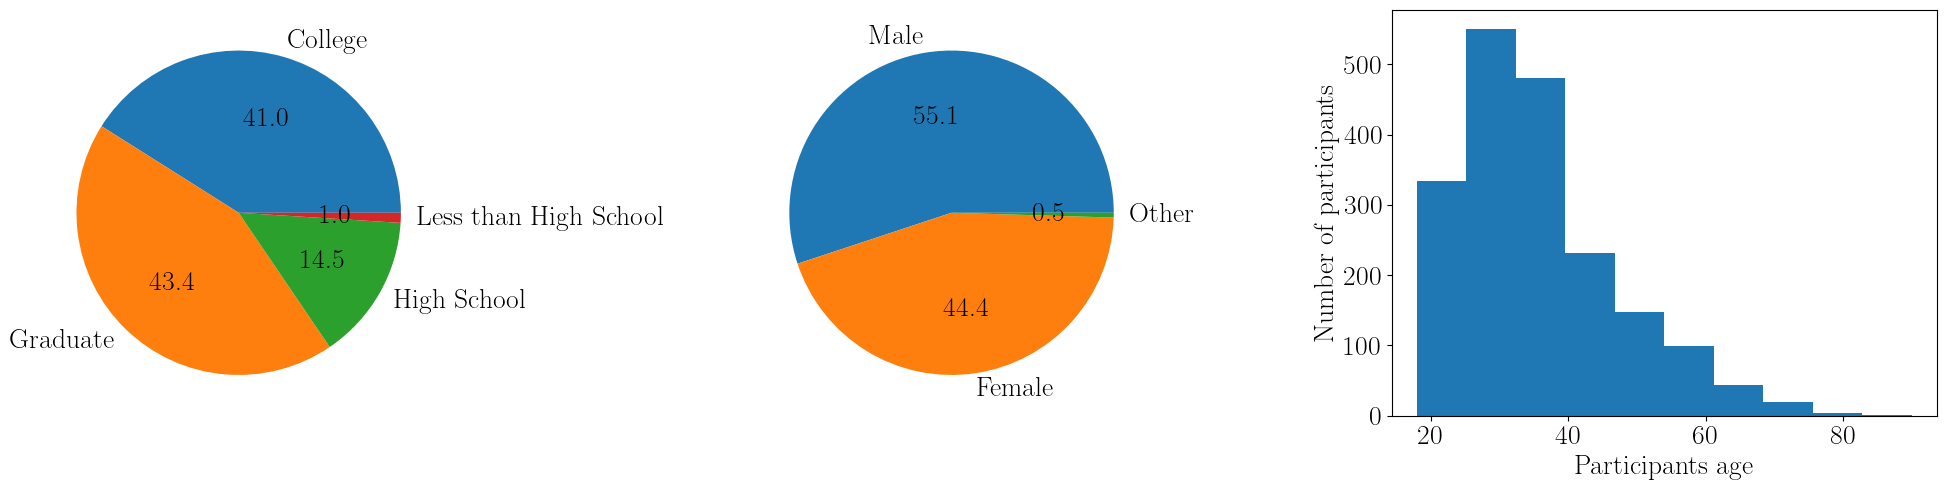
\includegraphics[width=13cm,height=3cm]{experiment/dists.png}
\caption{Demographic age (left), gender (middle) and education (right) distribution.
}\label{fig:distribution}
\end{center}
\end{figure}



%%%%%%%%%%%%%%%%%%%%%%%%%%%%%%%%%%%

\section{Details omitted from Comparing input formats}\label{app:comparison}
\subsection{Response time}
Figure~\ref{fig:consistency_time} shows how long the consistency stage took. 

\begin{figure}[!h]
\begin{center}
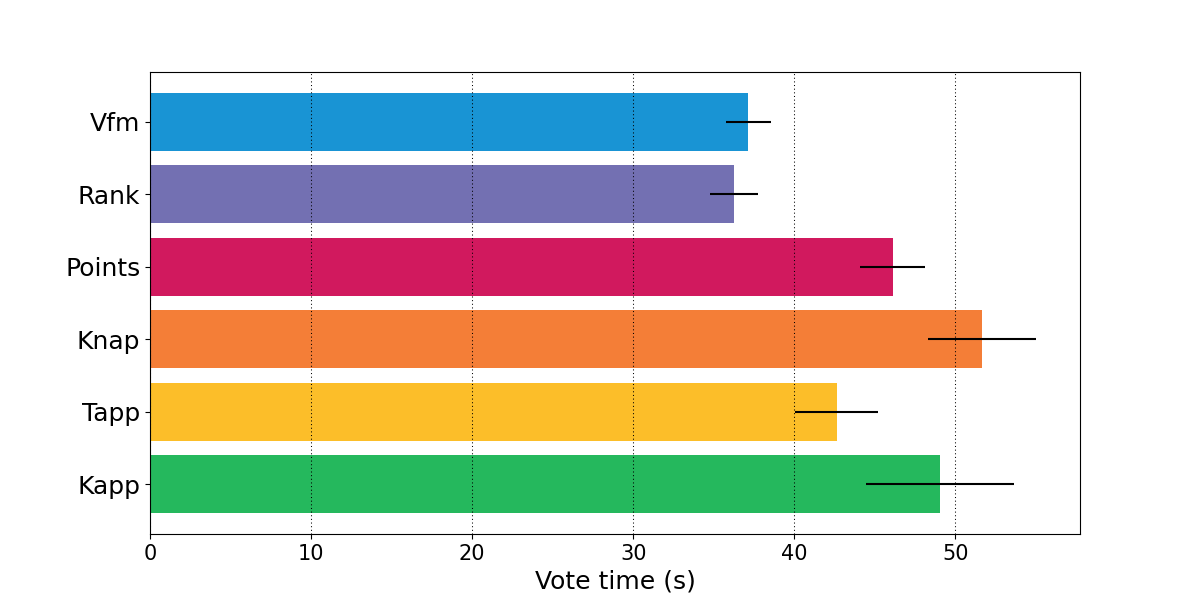
\includegraphics[width=7.5cm]{experiment/consistency_time.png}
\caption{How long it took the participants to do the consistency quiz (in seconds) on average.
}\label{fig:consistency_time}
\end{center}
\end{figure}


\subsection{Consistency}
Figures~\ref{fig:consistency_elections},\ref{fig:consistency} how many participants were consistent across different formats and across different project sets.%we collected in election and how many of them were consistent.. 
% \begin{figure}[!h]
% \begin{center}
% %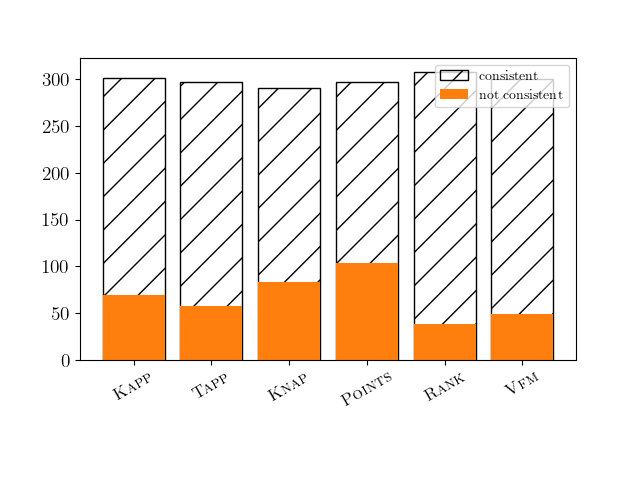
\includegraphics[width=7.5cm]{experiment/format_consistency.png}
% 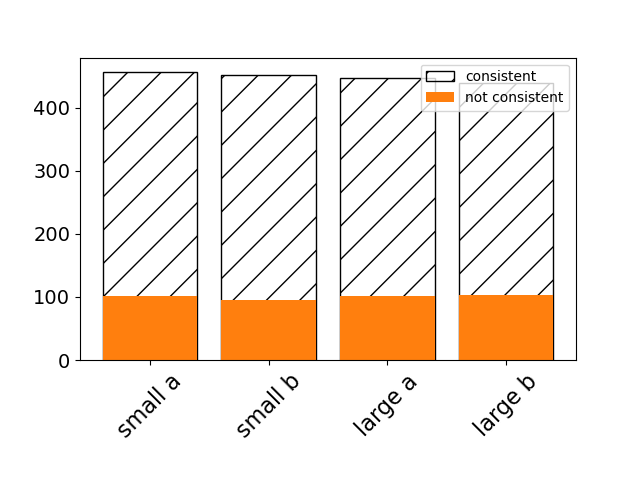
\includegraphics[width=7.5cm]{experiment/election_consistency.png}
% \caption{Total and consistent participants for each election.
% %\gb{should label elections properly eventually, not 3,6,etc. }
% }\label{fig:consistency_elections}
% \end{center}
% \end{figure}

% \begin{figure}[!h]
% \begin{center}
% 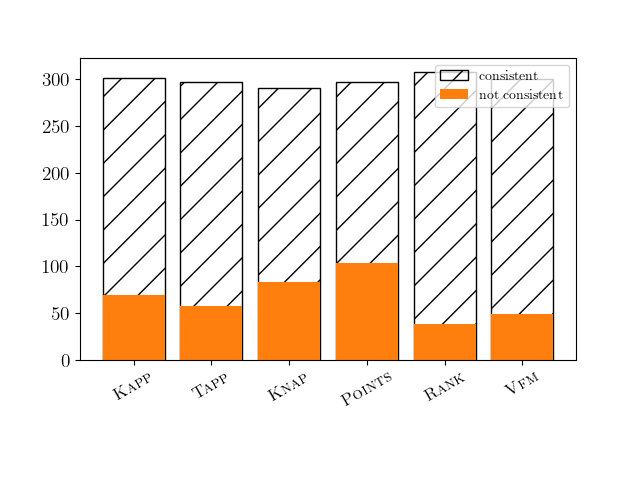
\includegraphics[width=7.5cm]{experiment/format_consistency.png}
% %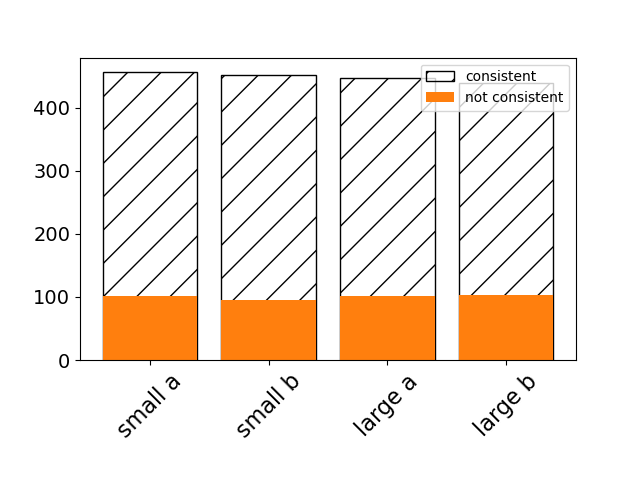
\includegraphics[width=7.5cm]{experiment/election_consistency.png}
% \caption{The total number of  participants who vote in each format, as well as the number that fail the consistency test.  Numbers are aggregated across elections. 
% %\gb{should label elections properly eventually, not 3,6,etc. }
% }\label{fig:consistency}%\rf{I think figure can be removed, read comment in the consistency subsection}
% \end{center}
% \end{figure}



\begin{figure*}[ht!]
     \centering
          \begin{subfigure}[b]{0.45\textwidth}
         \centering
       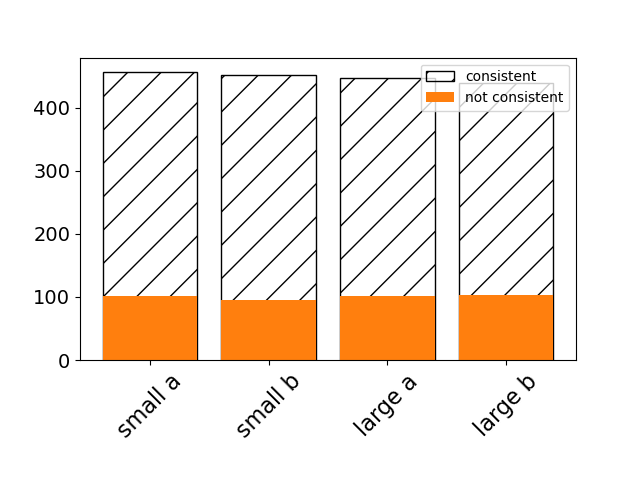
\includegraphics[width=6cm]{experiment/election_consistency.png}
\caption{The total number of  participants who vote in each election, as well as the number that fail the consistency test.  Numbers are aggregated across formats.
}\label{fig:consistency_elections}
     \end{subfigure}\hfill
     \begin{subfigure}[b]{0.45\textwidth}
         \centering
         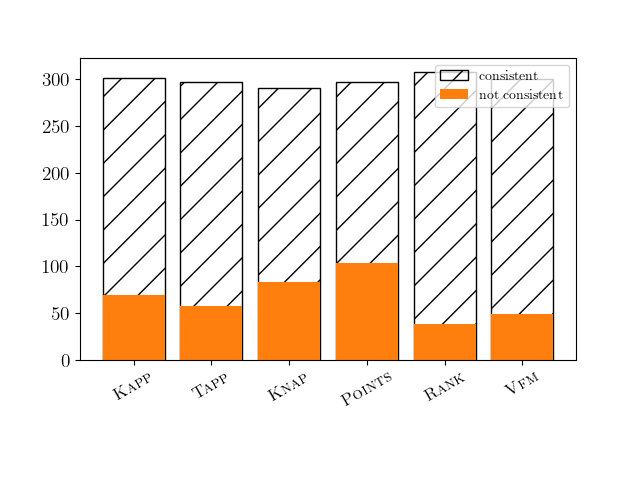
\includegraphics[width=6cm]{experiment/format_consistency.png}
\caption{The total number of  participants who vote in each format, as well as the number that fail the consistency test.  Numbers are aggregated across elections.
}\label{fig:consistency}
     \end{subfigure}
        \caption{Input formats and elections consistency.}
        \label{fig:all_consistency}
\end{figure*}

%%%%%%%%%%%%%%%%%%%%%%%%%%%%%%%%%

\section{Entropy}\label{app:entropy}
Figures~\ref{fig:entropy_sa}-\ref{fig:entropy_lb}  shows the entropy for all of the project sets, all input formats when using greedy and \mes{}, given different sample size. 


\begin{figure*}[!h]
     \centering
          \begin{subfigure}[b]{0.45\textwidth}
         \centering
        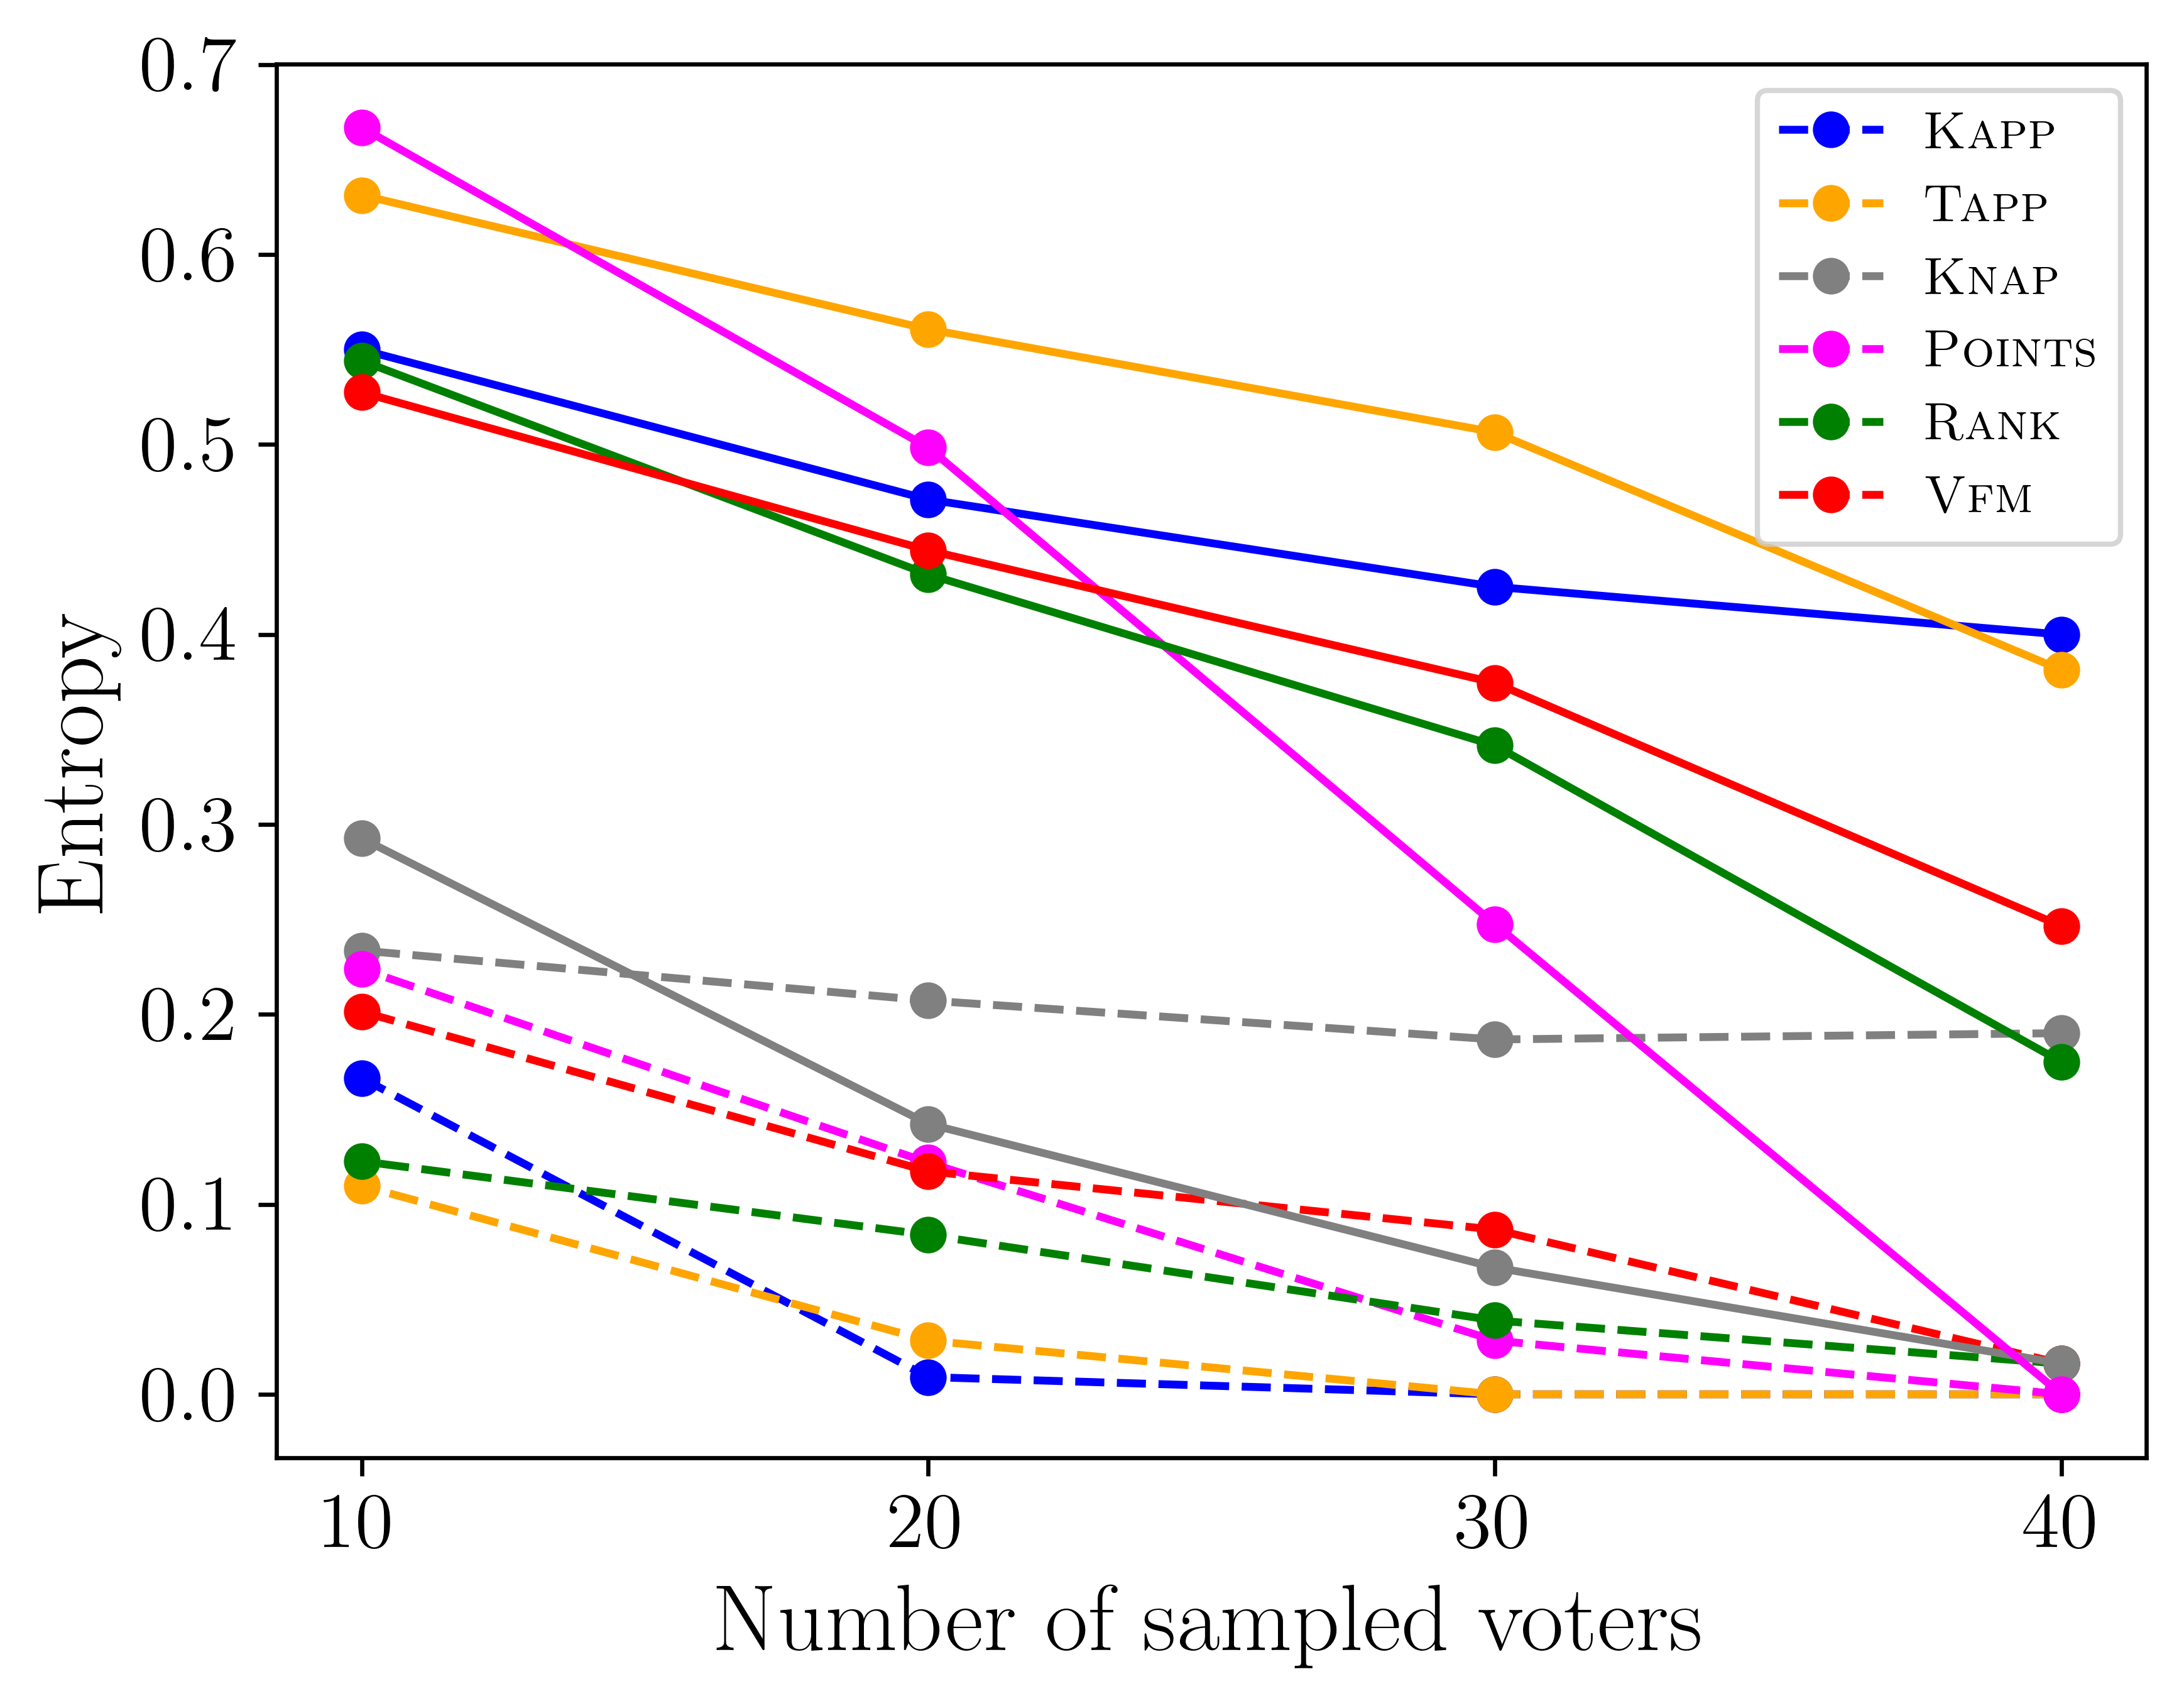
\includegraphics[width=6cm]{experiment/entropy_small_a.png}
\caption{Greedy (full lines) and \mes (dotted lines) entropy  for each input format (sample format get same color) given different sample size in project set \textsc{Small-A} }\label{fig:entropy_sa}
     \end{subfigure}\hfill
     \begin{subfigure}[b]{0.45\textwidth}
         \centering
         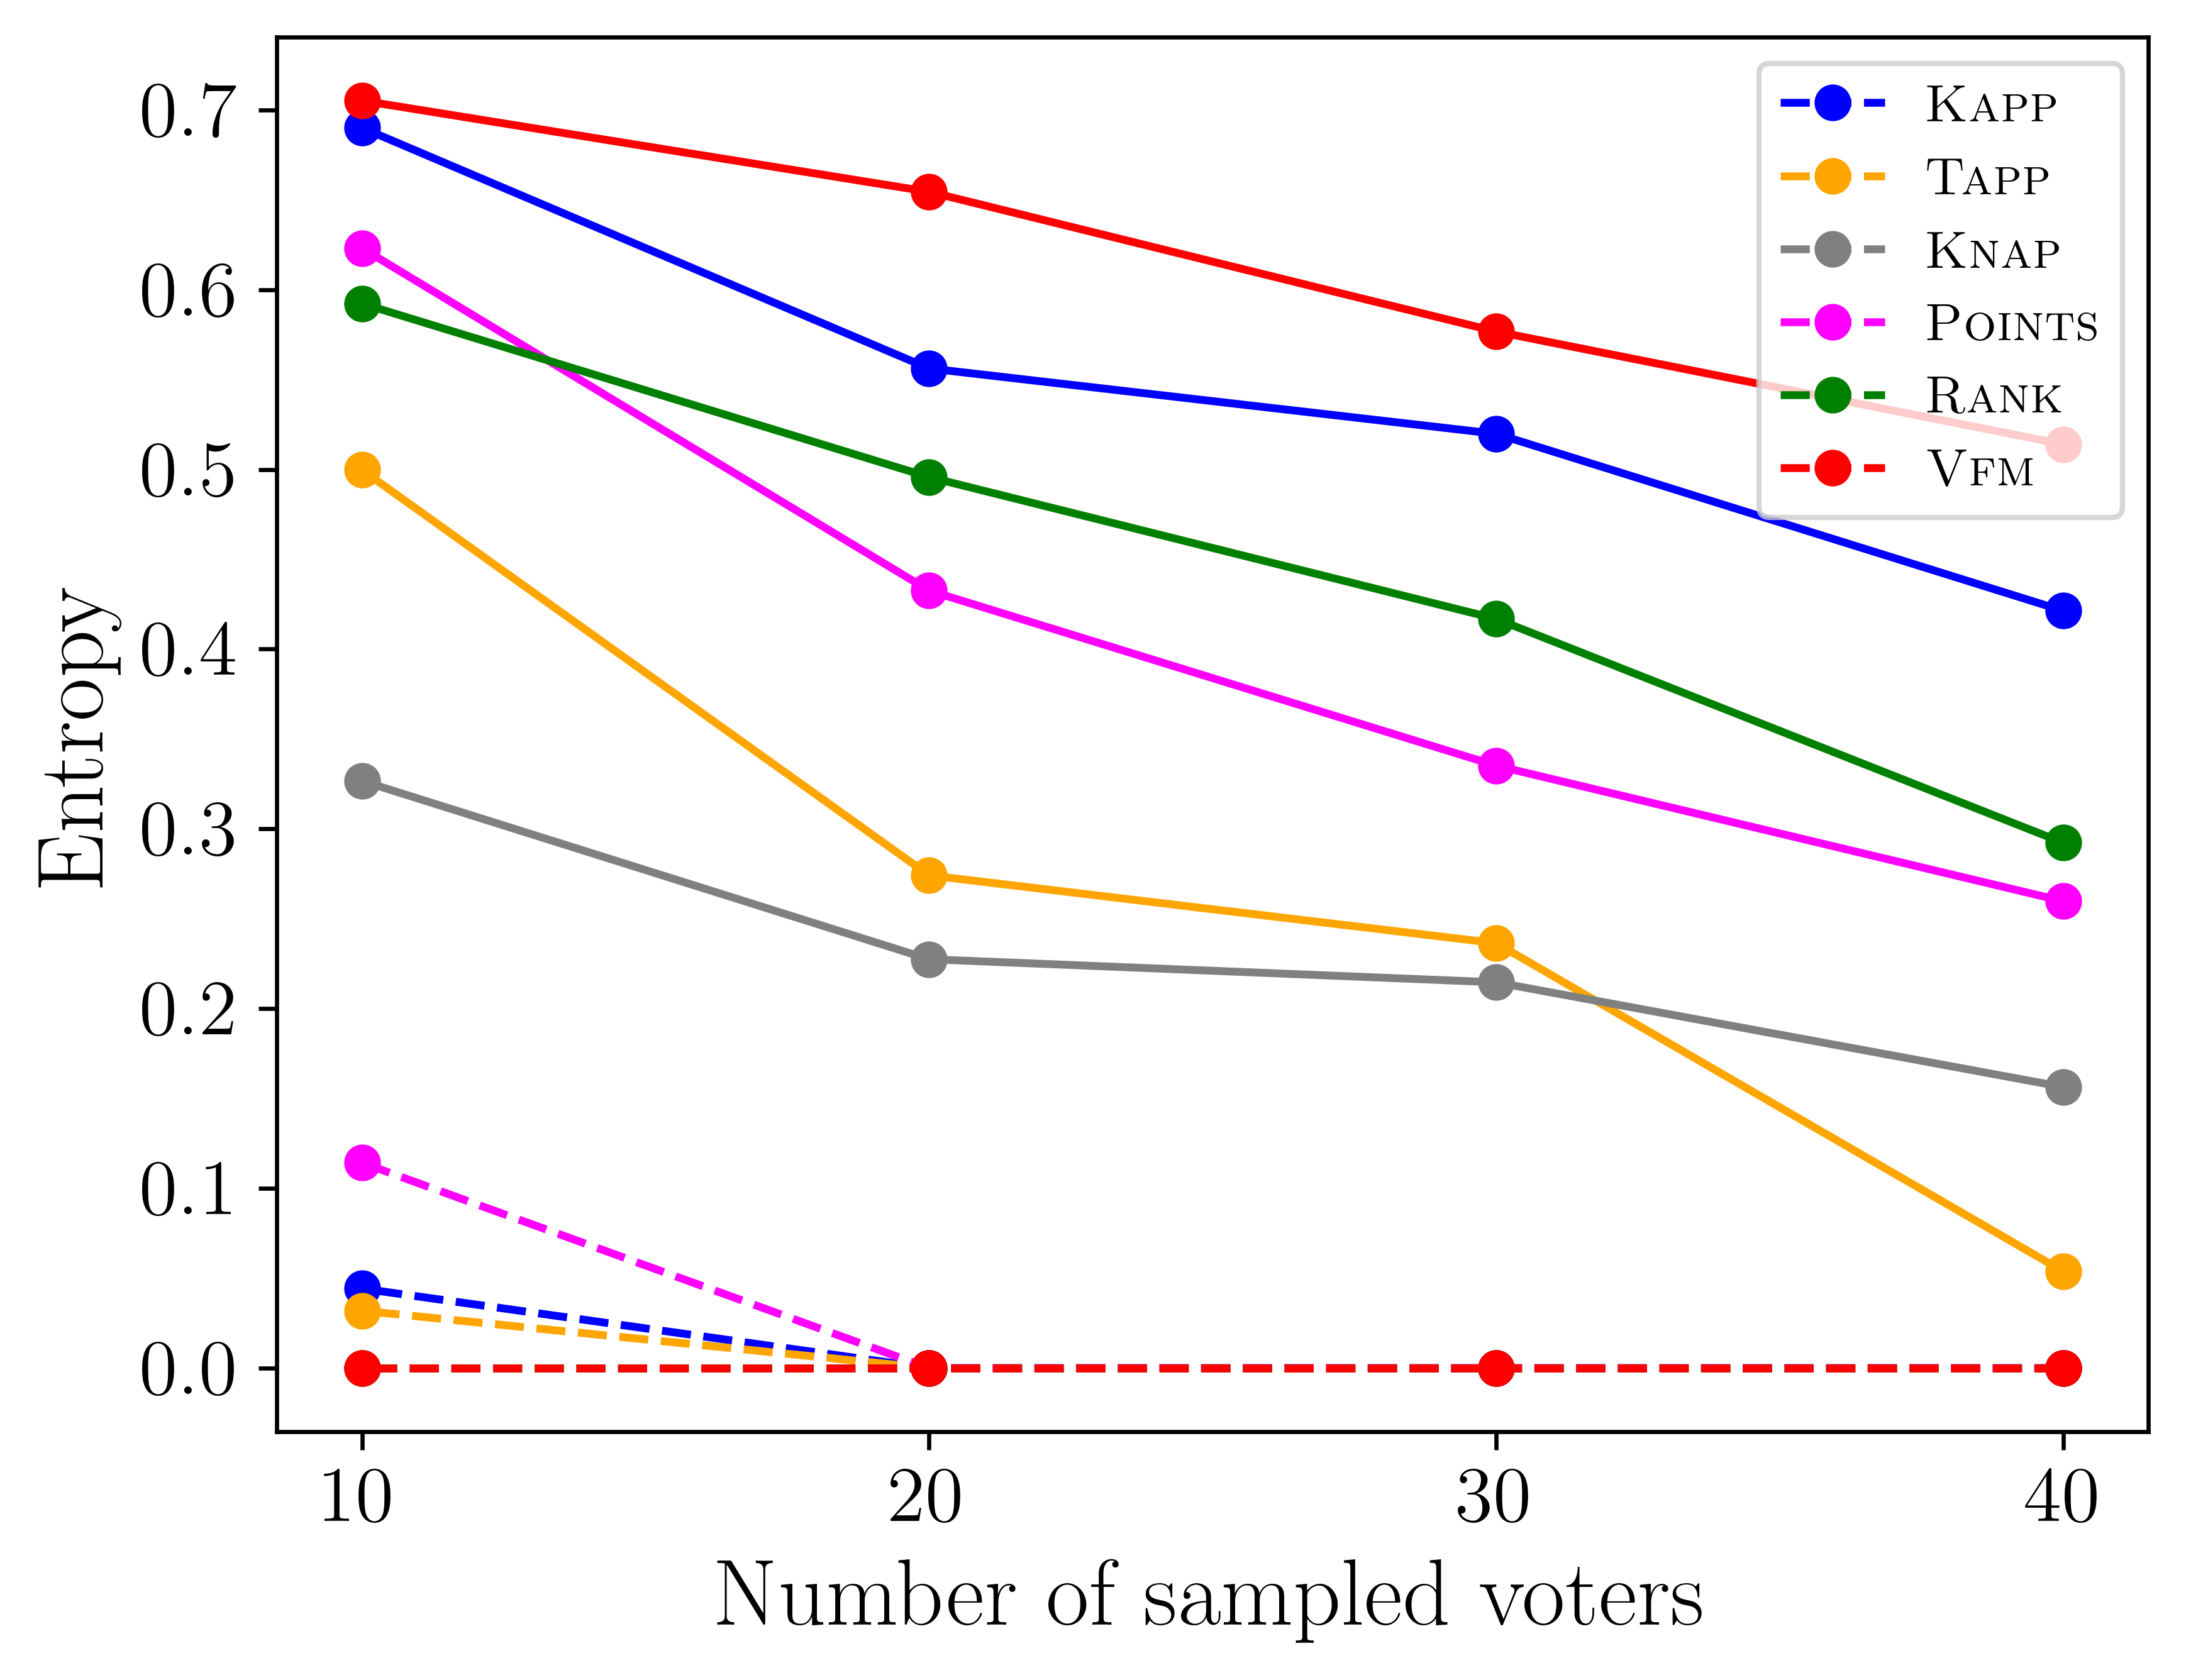
\includegraphics[width=6cm]{experiment/entropy_small_b.png}
\caption{Greedy (full lines) and \mes (dotted lines) entropy  for each input format (sample format get same color) given different sample size in project set \textsc{Small-B}}\label{fig:entropy_sb}
     \end{subfigure}
     \hfill
     \begin{subfigure}[b]{0.45\textwidth}
         \centering
         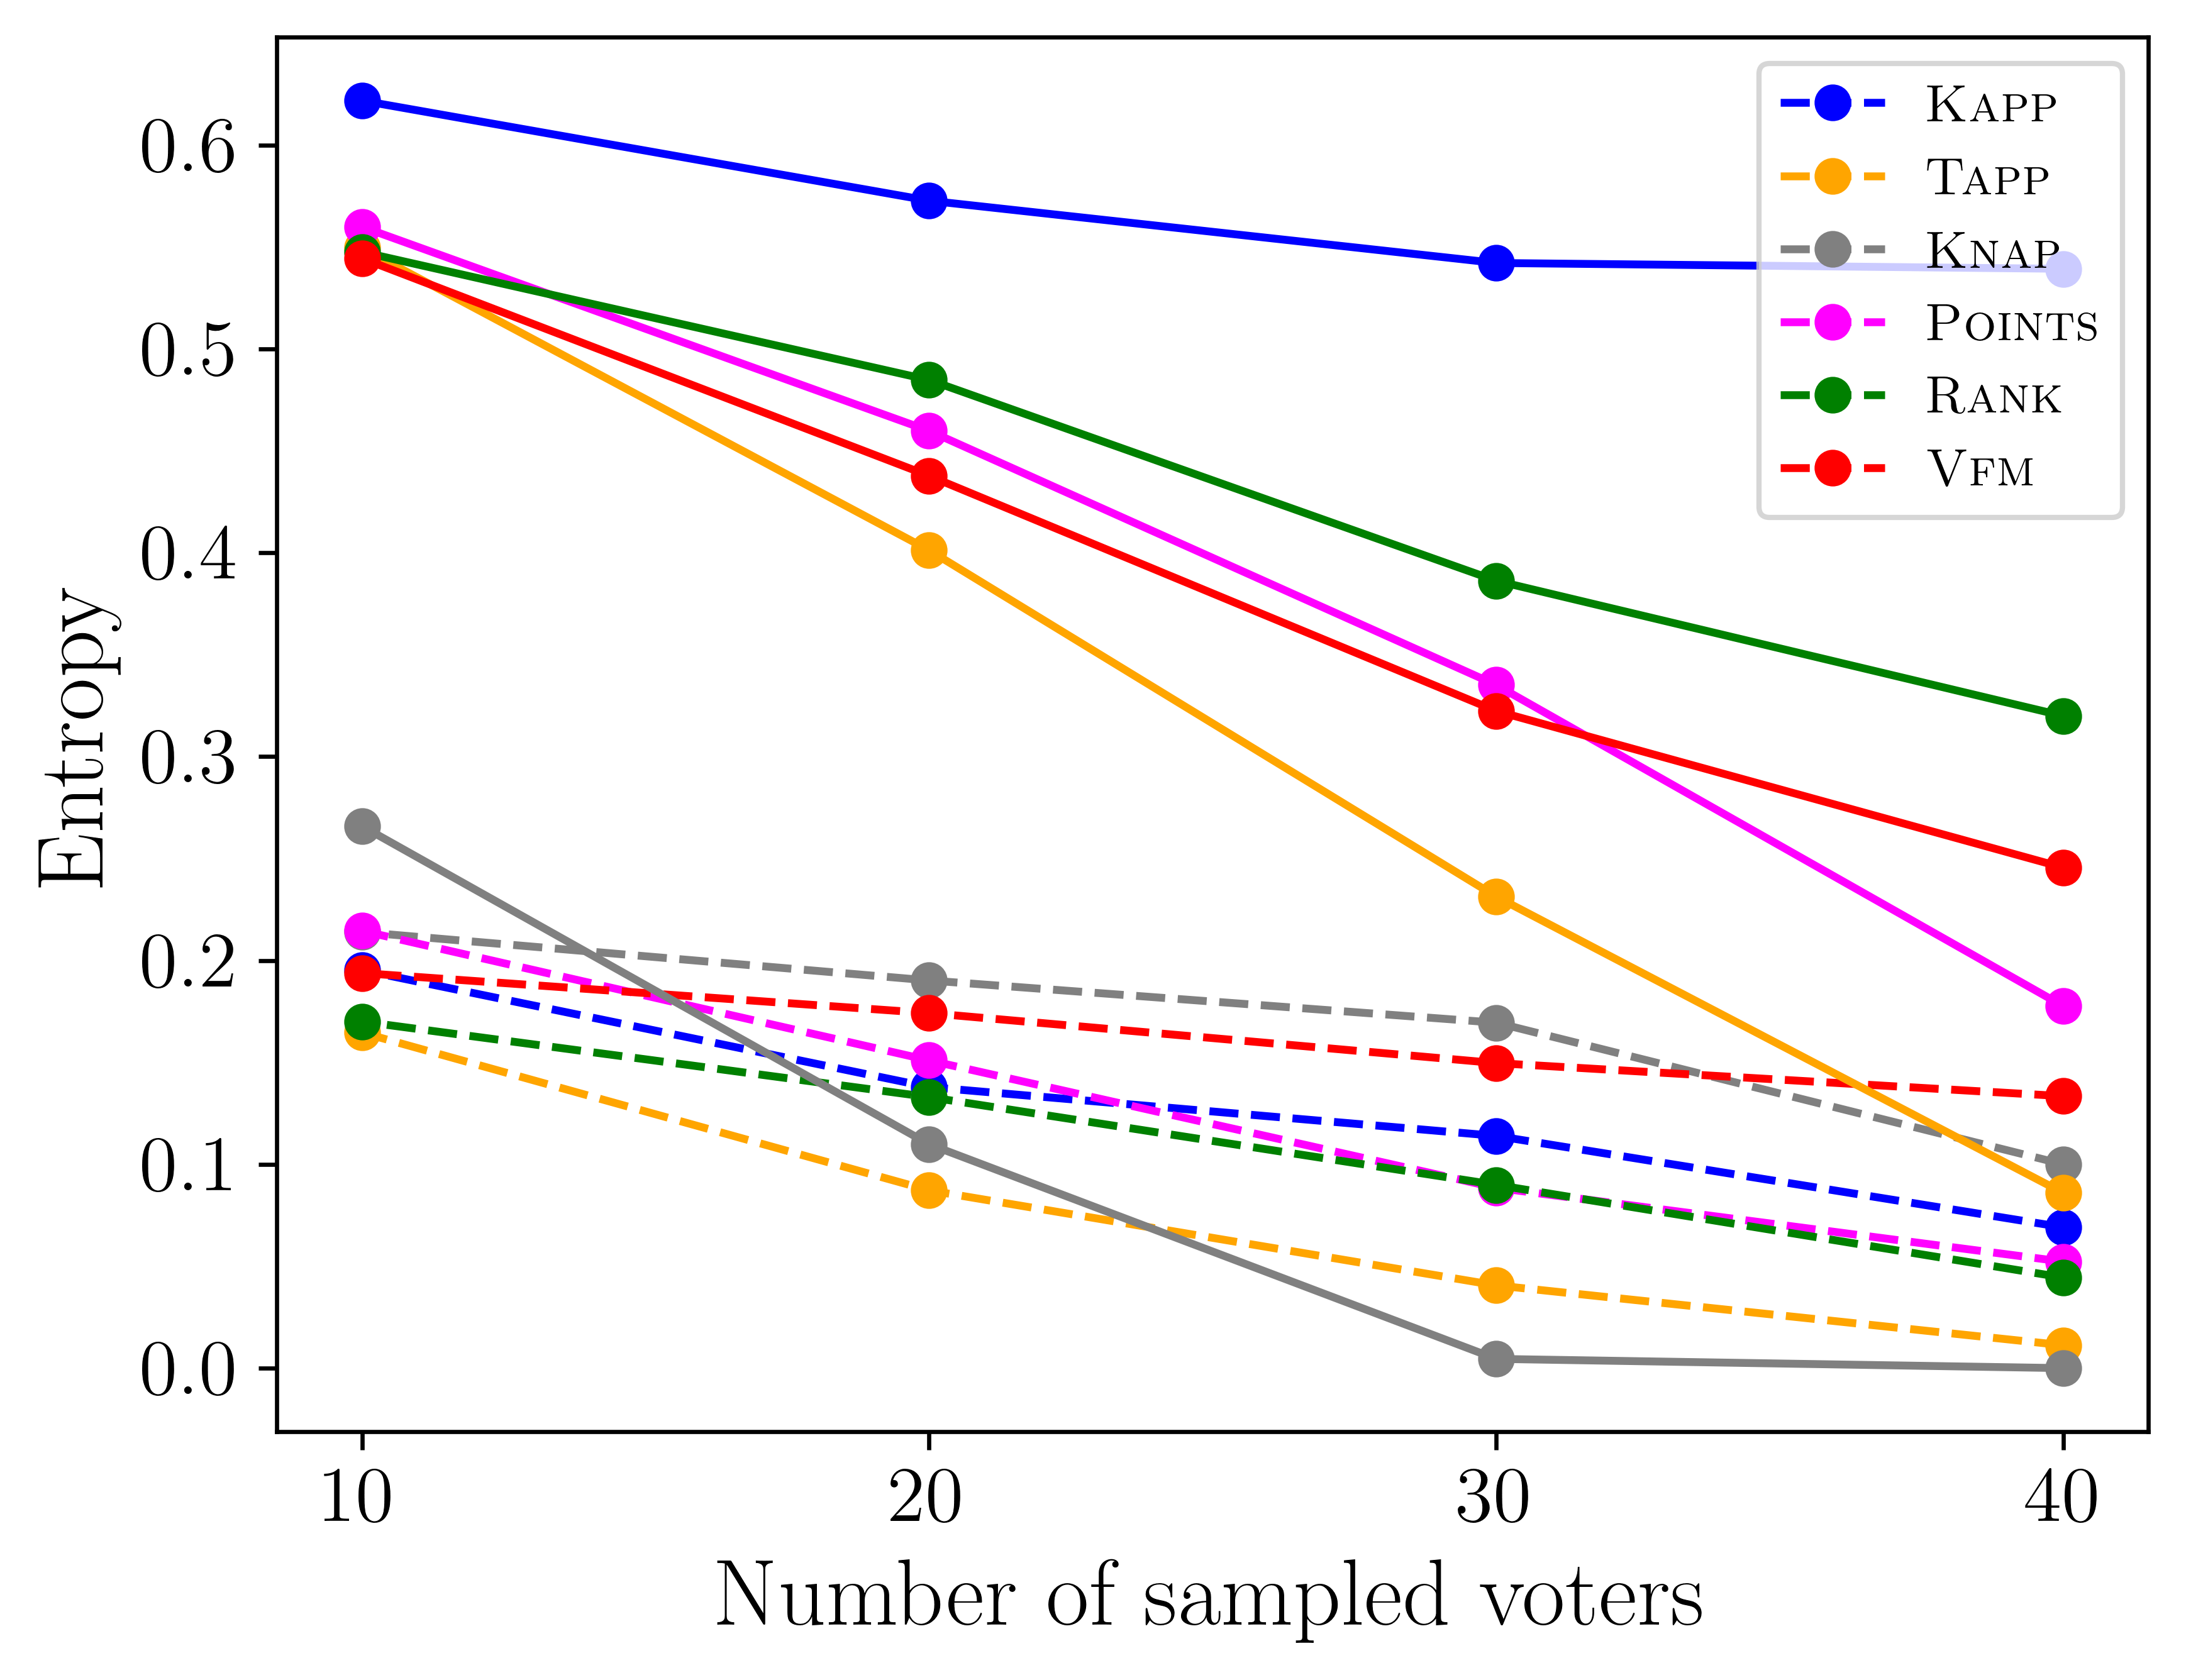
\includegraphics[width=6cm]{experiment/entropy_large_a.png}
\caption{Greedy (full lines) and \mes (dotted lines) entropy  for each input format (sample format get same color) given different sample size in project set \textsc{Large-A} }\label{fig:entropy_la}
     \end{subfigure}
     \hfill
     \begin{subfigure}[b]{0.45\textwidth}
         \centering
         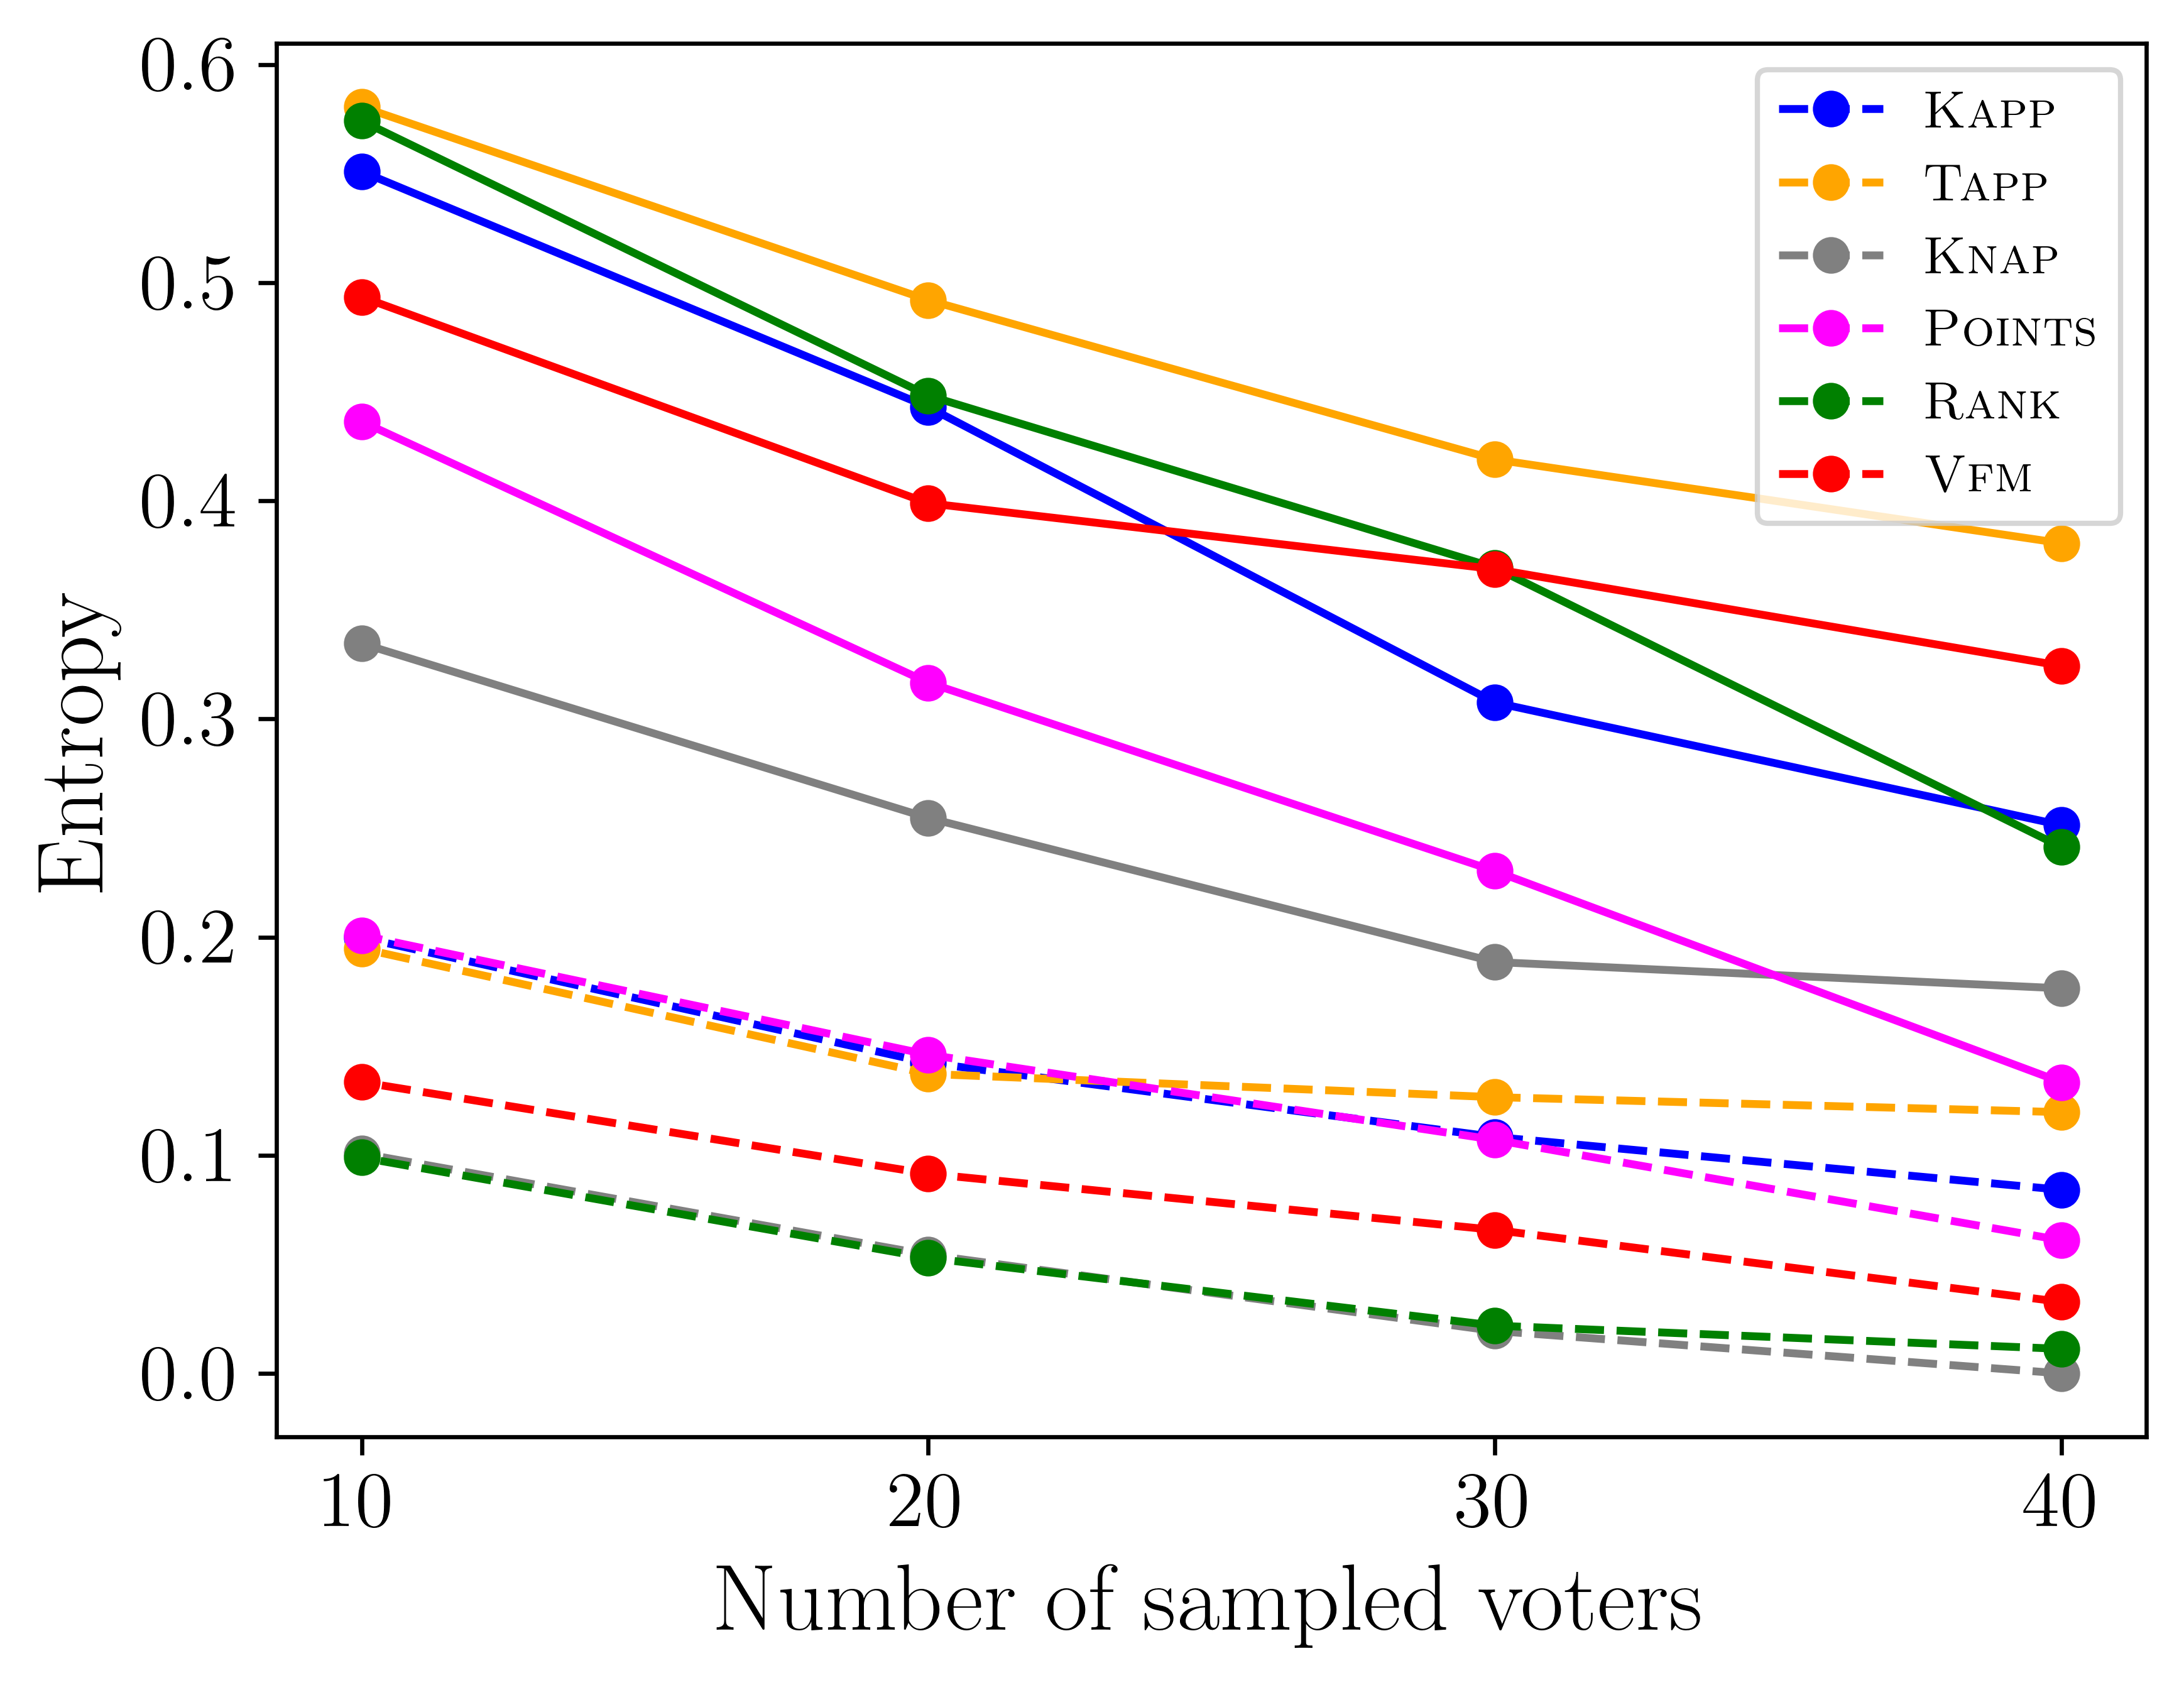
\includegraphics[width=6cm]{experiment/entropy_large_b.png}
\caption{Greedy (full lines) and \mes (dotted lines) entropy  for each input format (sample format get same color) given different sample size in project set \textsc{Large-B} }\label{fig:entropy_lb}
     \end{subfigure}

        \caption{Entropy for each of the elections.}
        \label{fig:app_entropy}
\end{figure*}

%%%%%%%%%%%%%%%%%%%%%%%%%%%%%%%%%55
% \clearpage

\section{Welfare from all formats voters}\label{app:aggregation}
Figures~\ref{fig:kapp_welfare}-\ref{fig:util_welfare} shows the welfare (averaged across elections), when using each of the input formats voters to calculate the welfare.


% \begin{figure}[!ht]
% \begin{center}
% 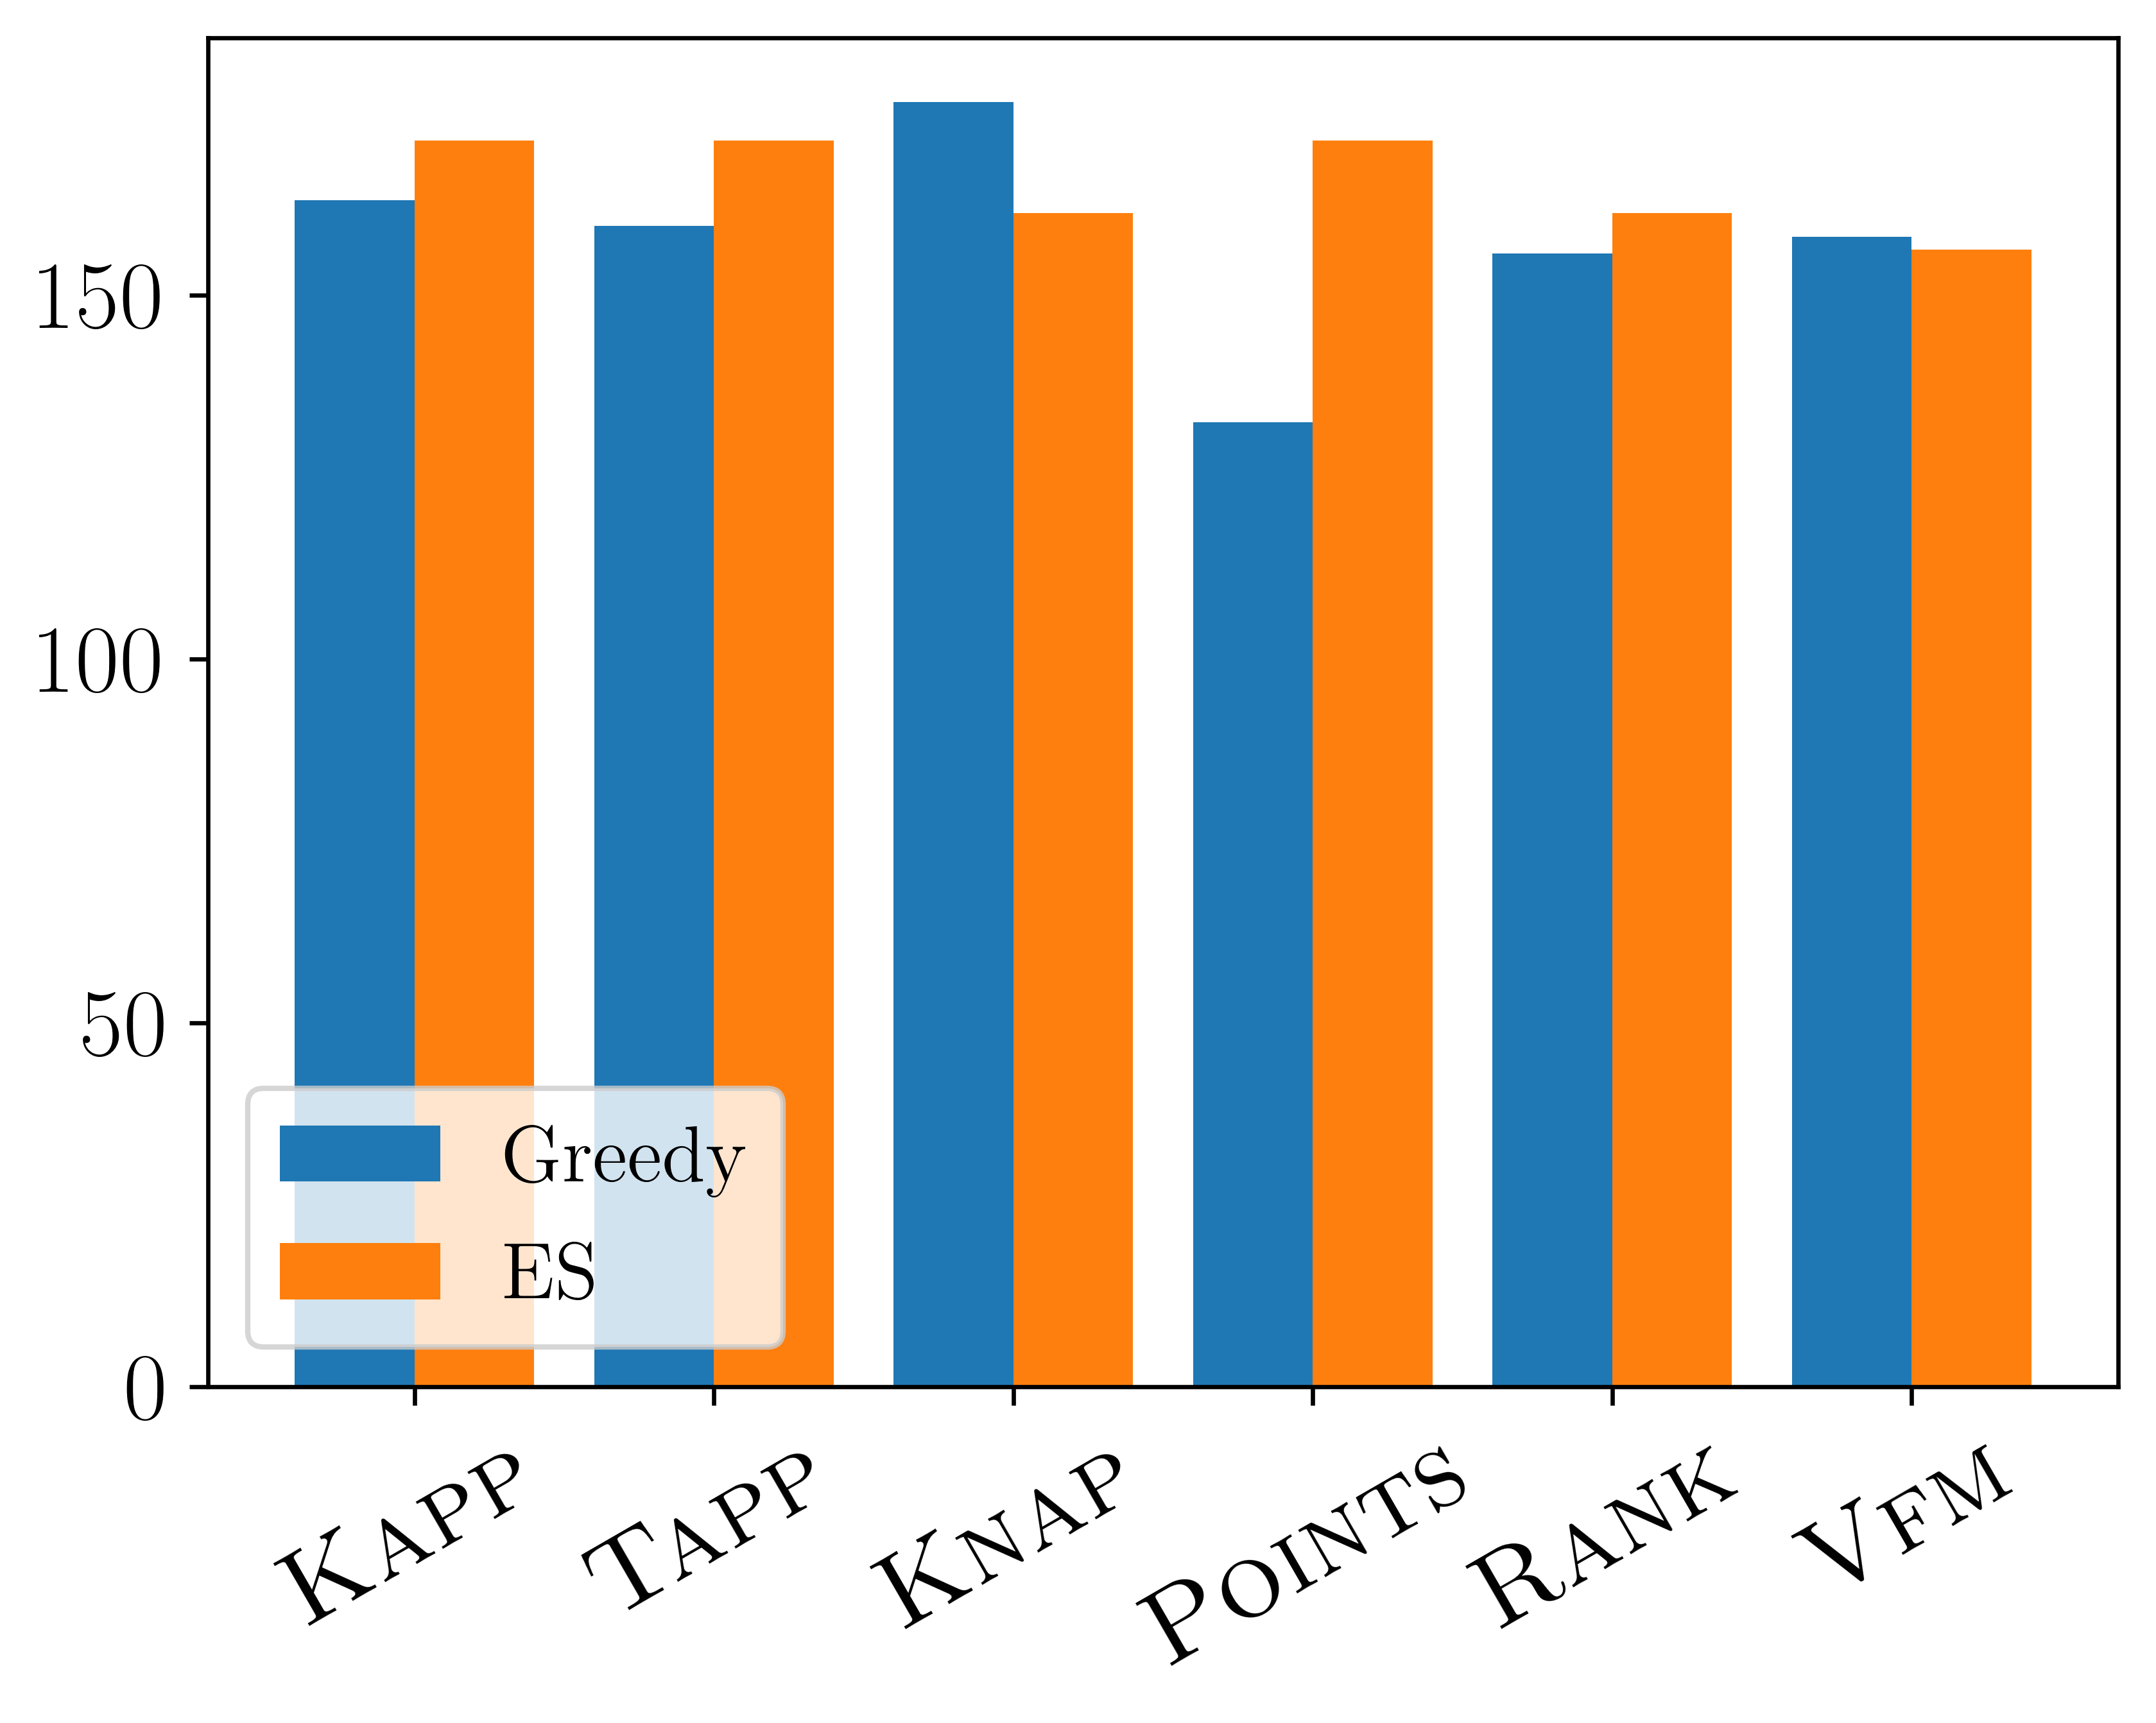
\includegraphics[width=7.5cm]{experiment/k_approval_welfare.png}
% \caption{Average social welfare (averaged across elections) using \kapp{}-voters to compute welfare.
% }\label{fig:kapp_welfare}
% \end{center}
% \end{figure}

% \begin{figure}[!ht]
% \begin{center}
% 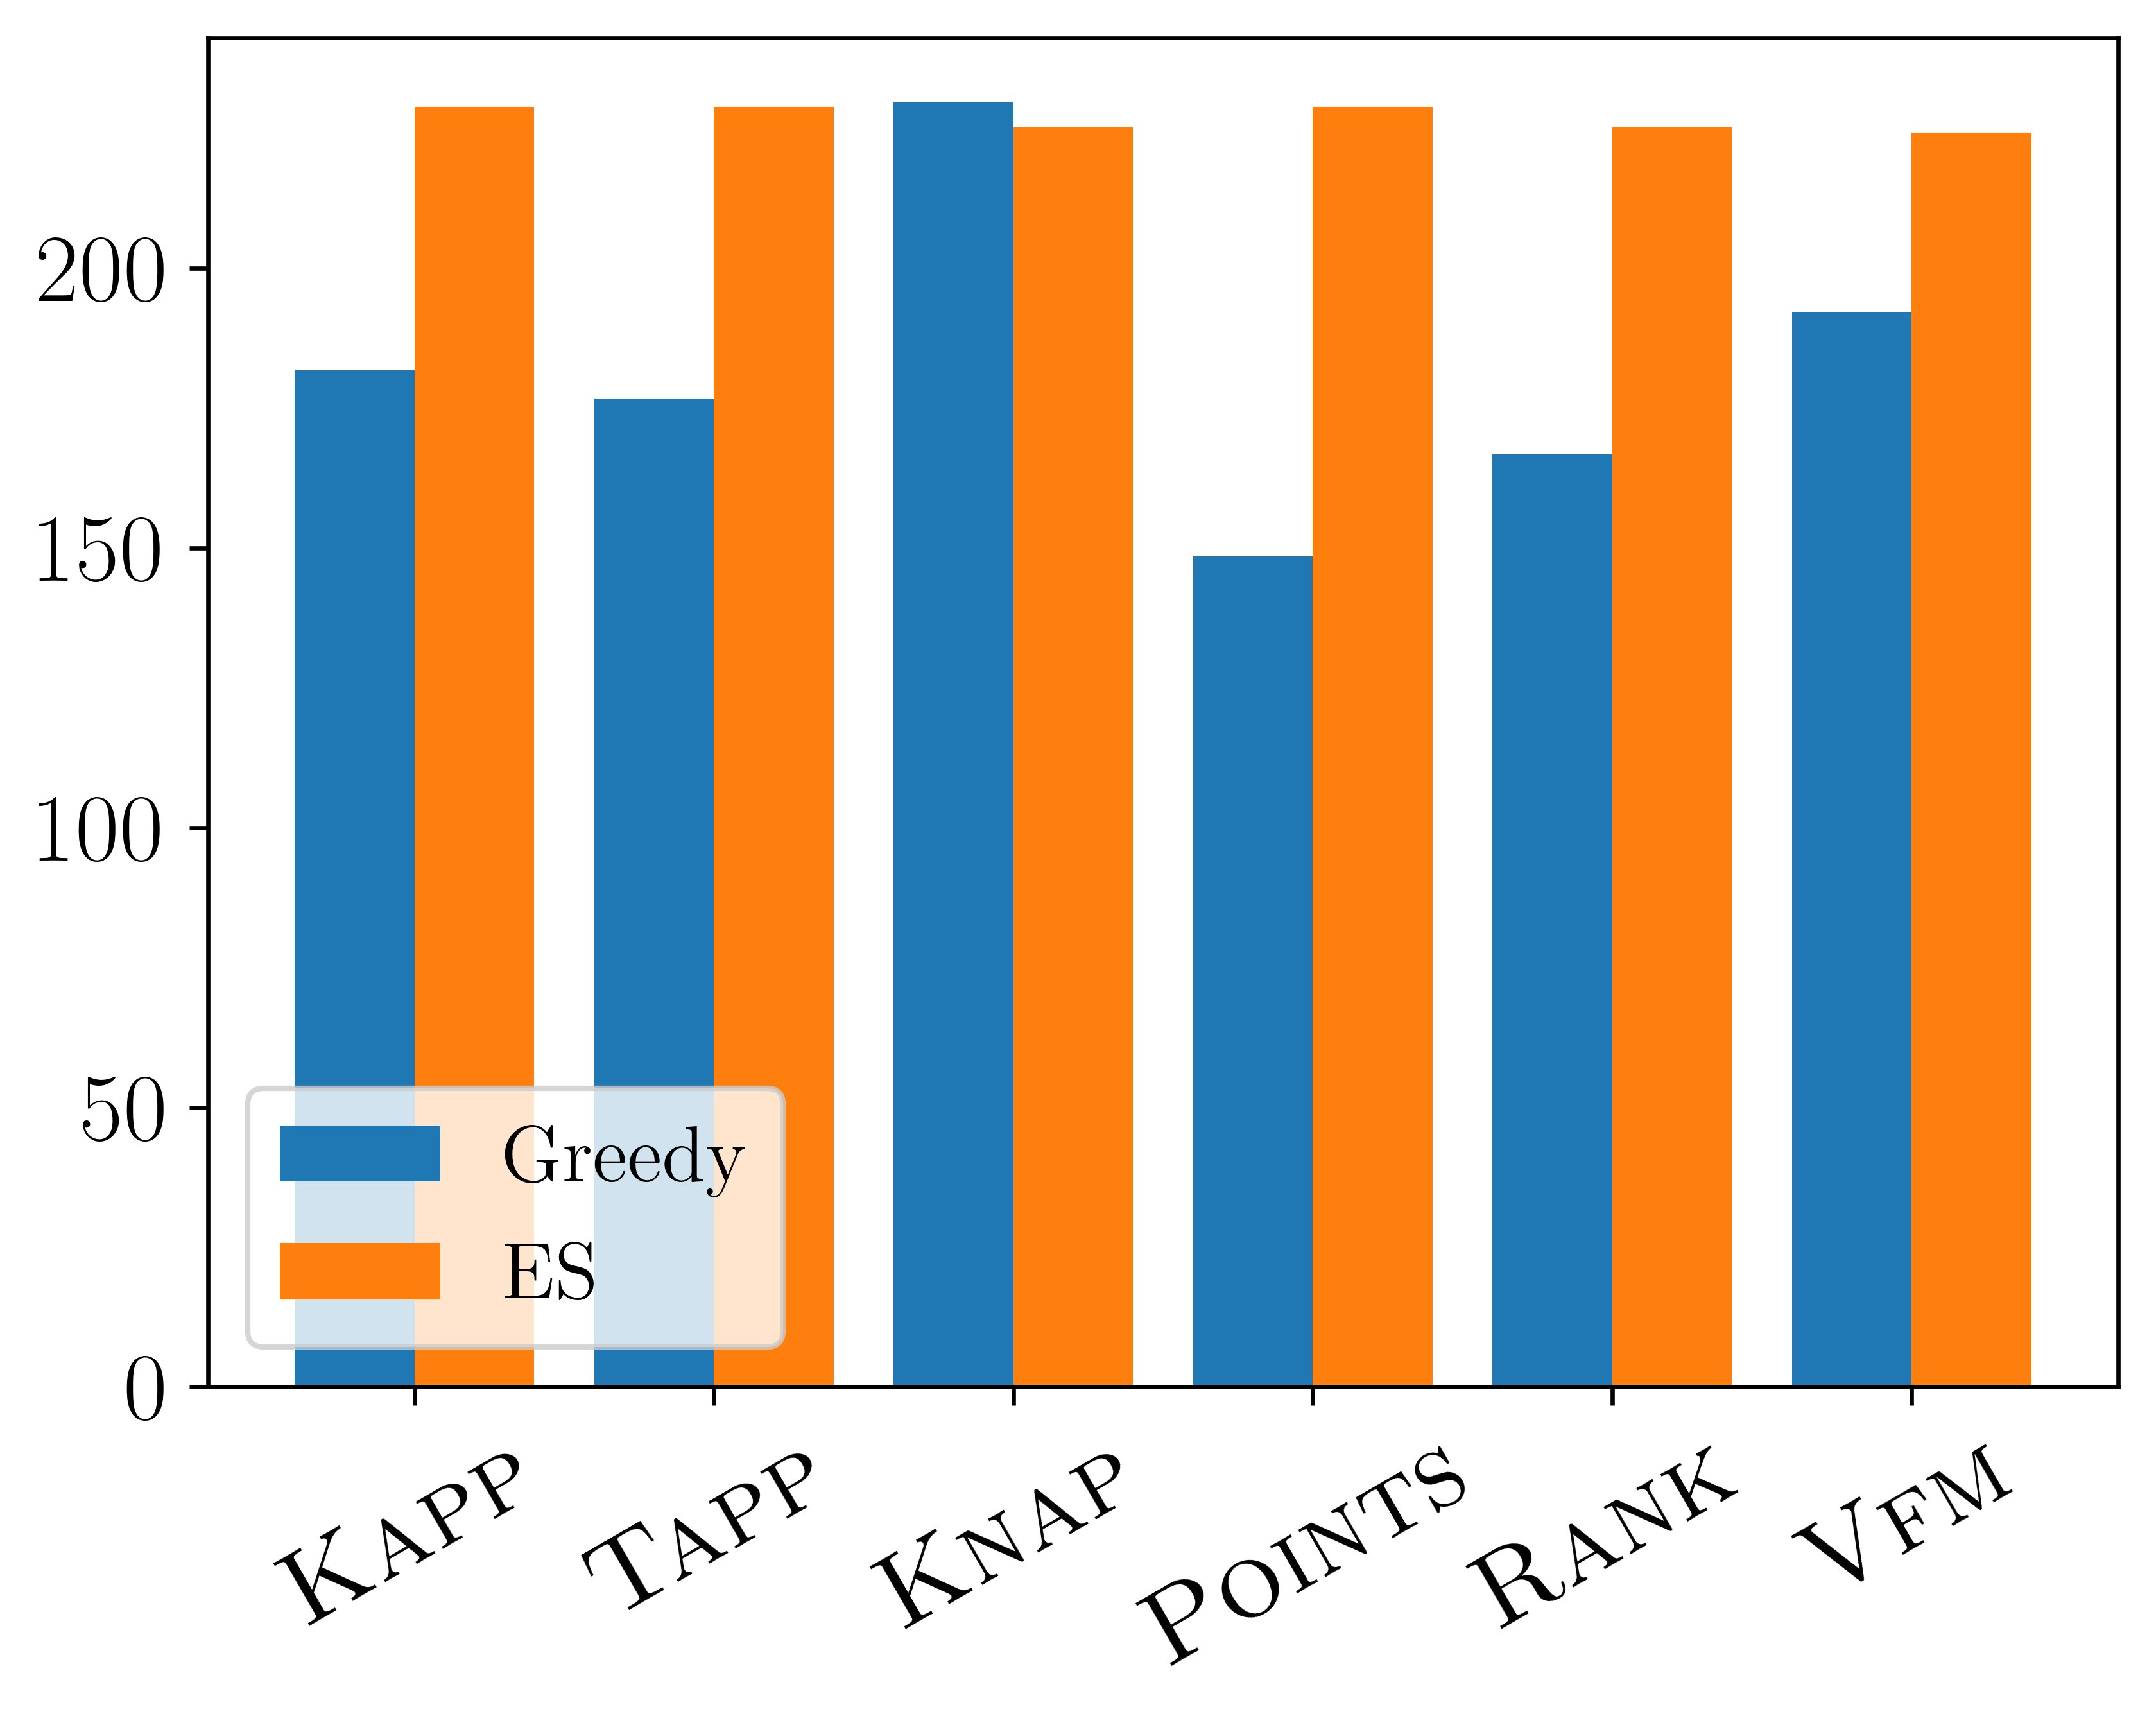
\includegraphics[width=7.5cm]{experiment/Knapsack_welfare.png}
% \caption{Average social welfare (averaged across elections) using \knap{}-voters to compute welfare.
% }\label{fig:knap_welfare}
% \end{center}
% \end{figure}

% \begin{figure}[!ht]
% \begin{center}
% 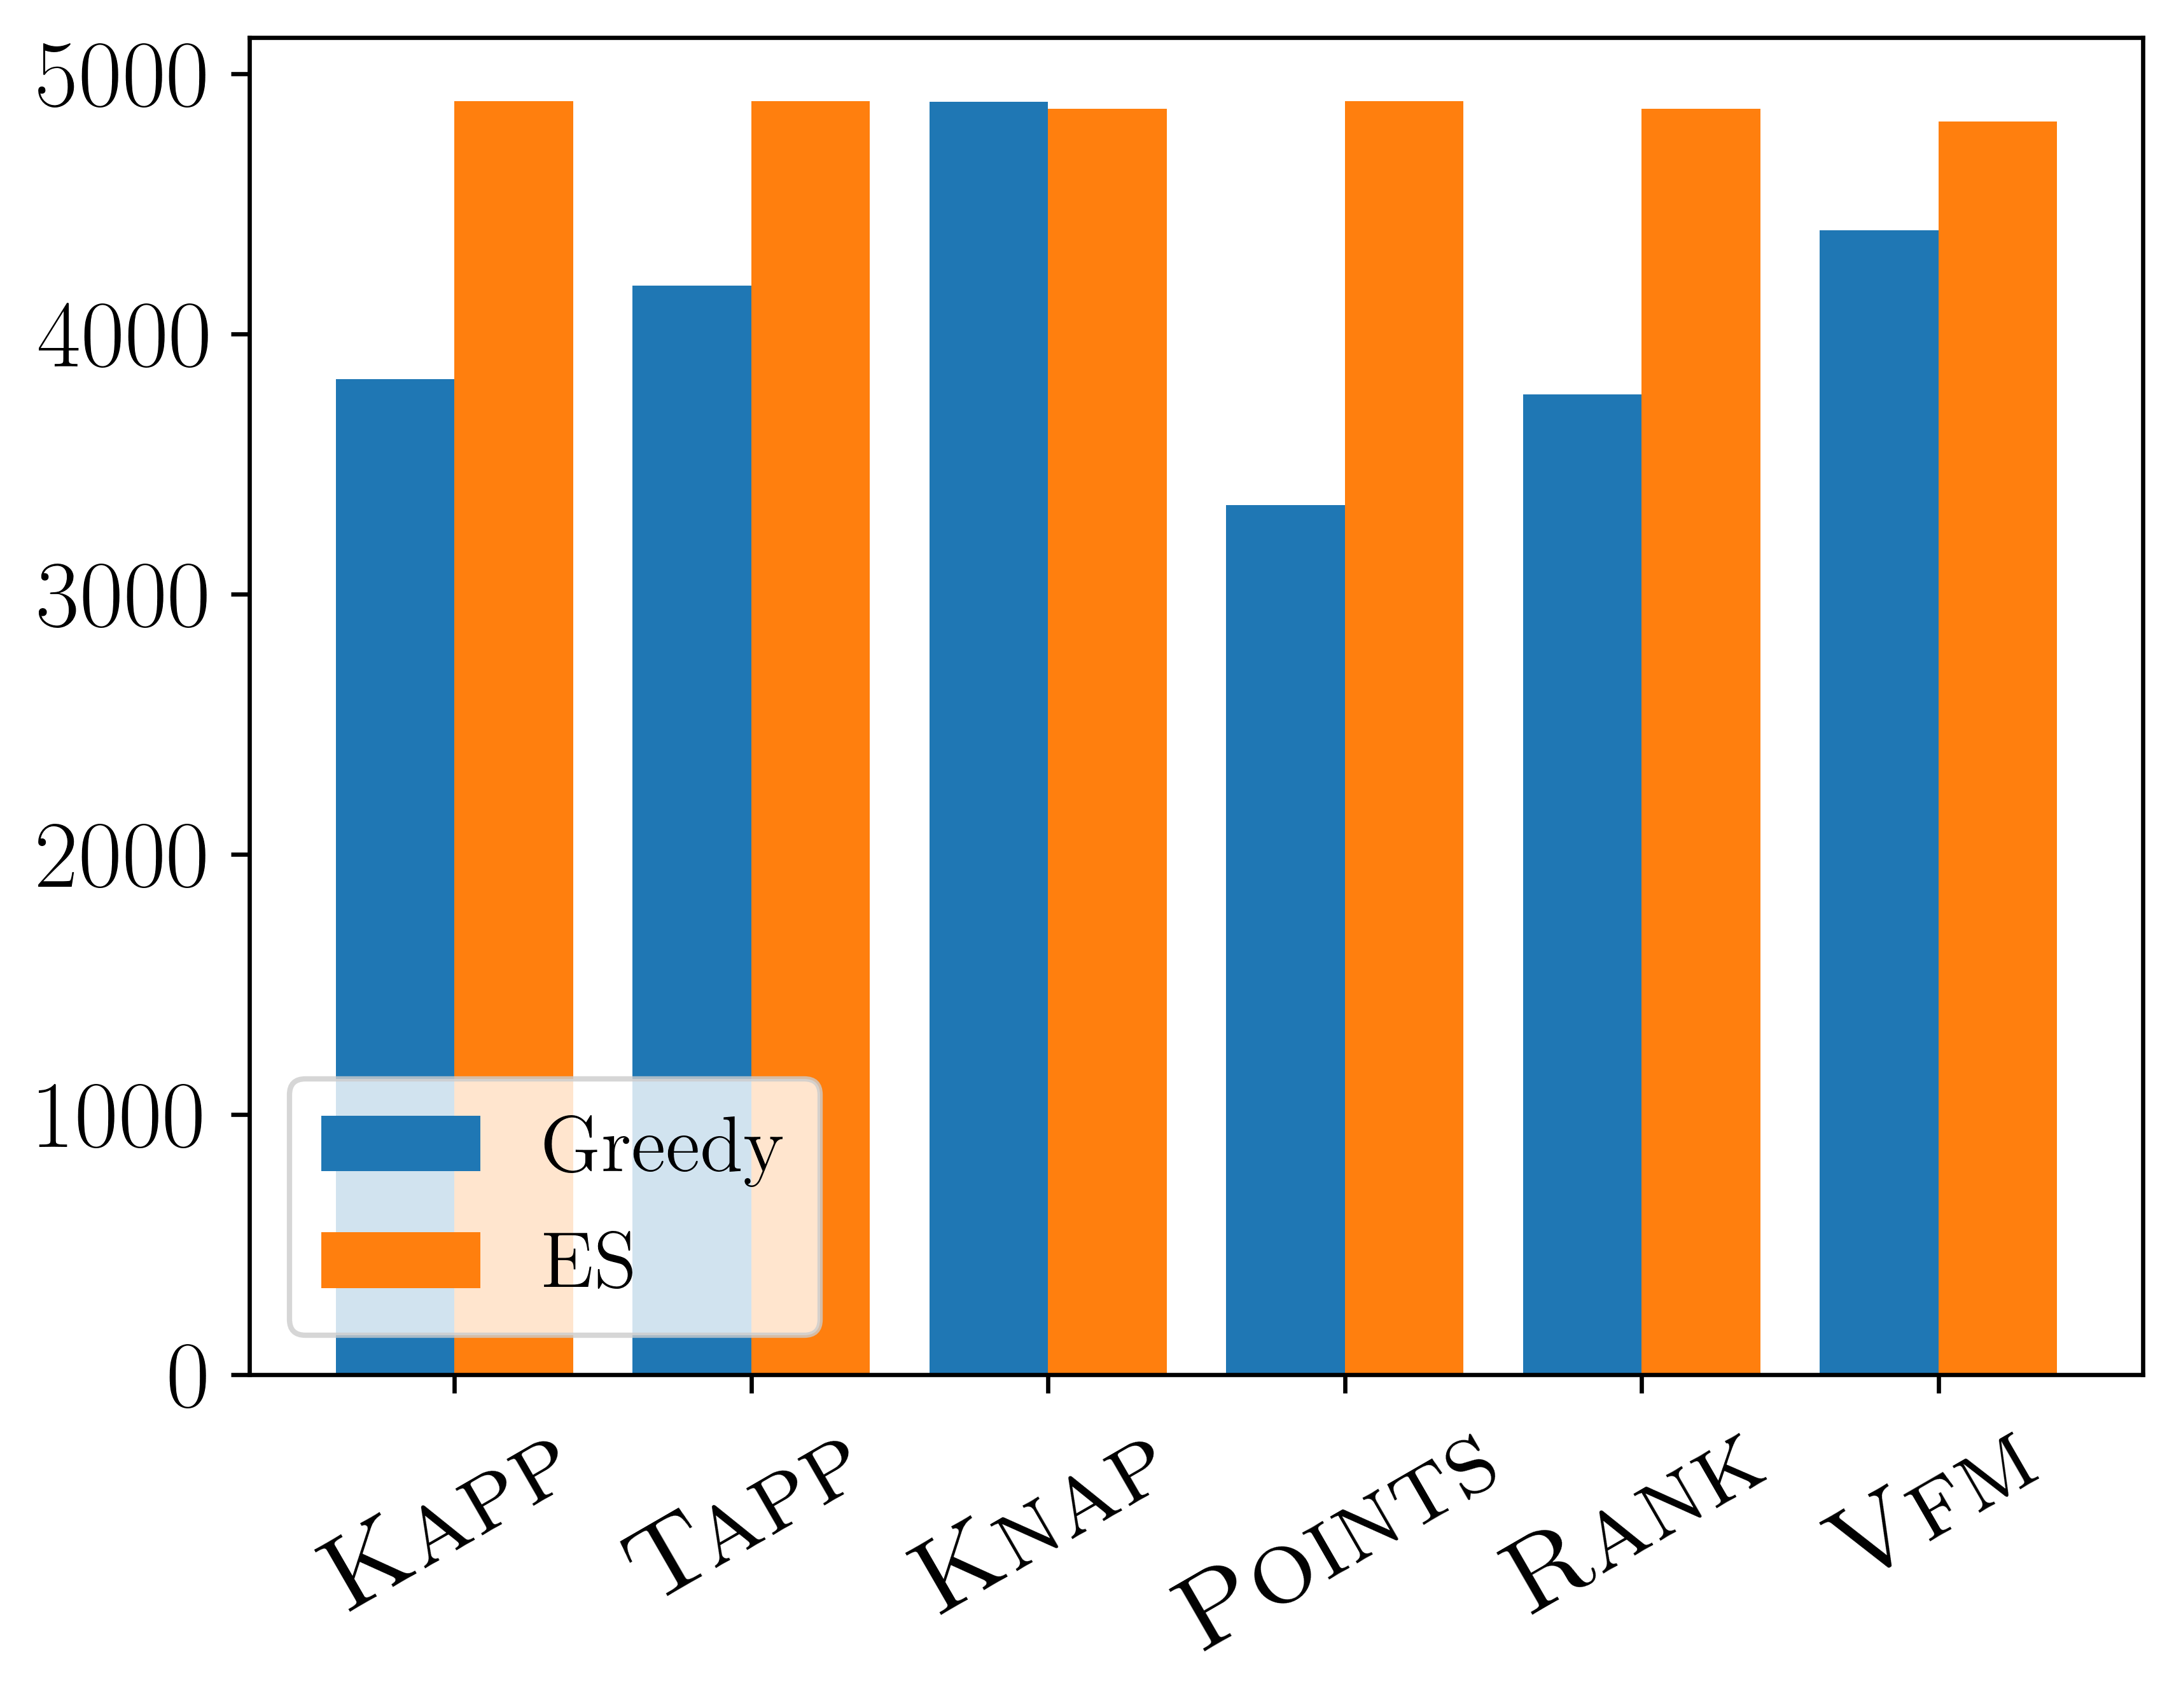
\includegraphics[width=7.5cm]{experiment/Ranking_value_welfare.png}
% \caption{Average social welfare (averaged across elections) using \rank{}-voters to compute welfare.
% }\label{fig:rank_welfare}
% \end{center}
% \end{figure}

% \begin{figure}[!ht]
% \begin{center}
% 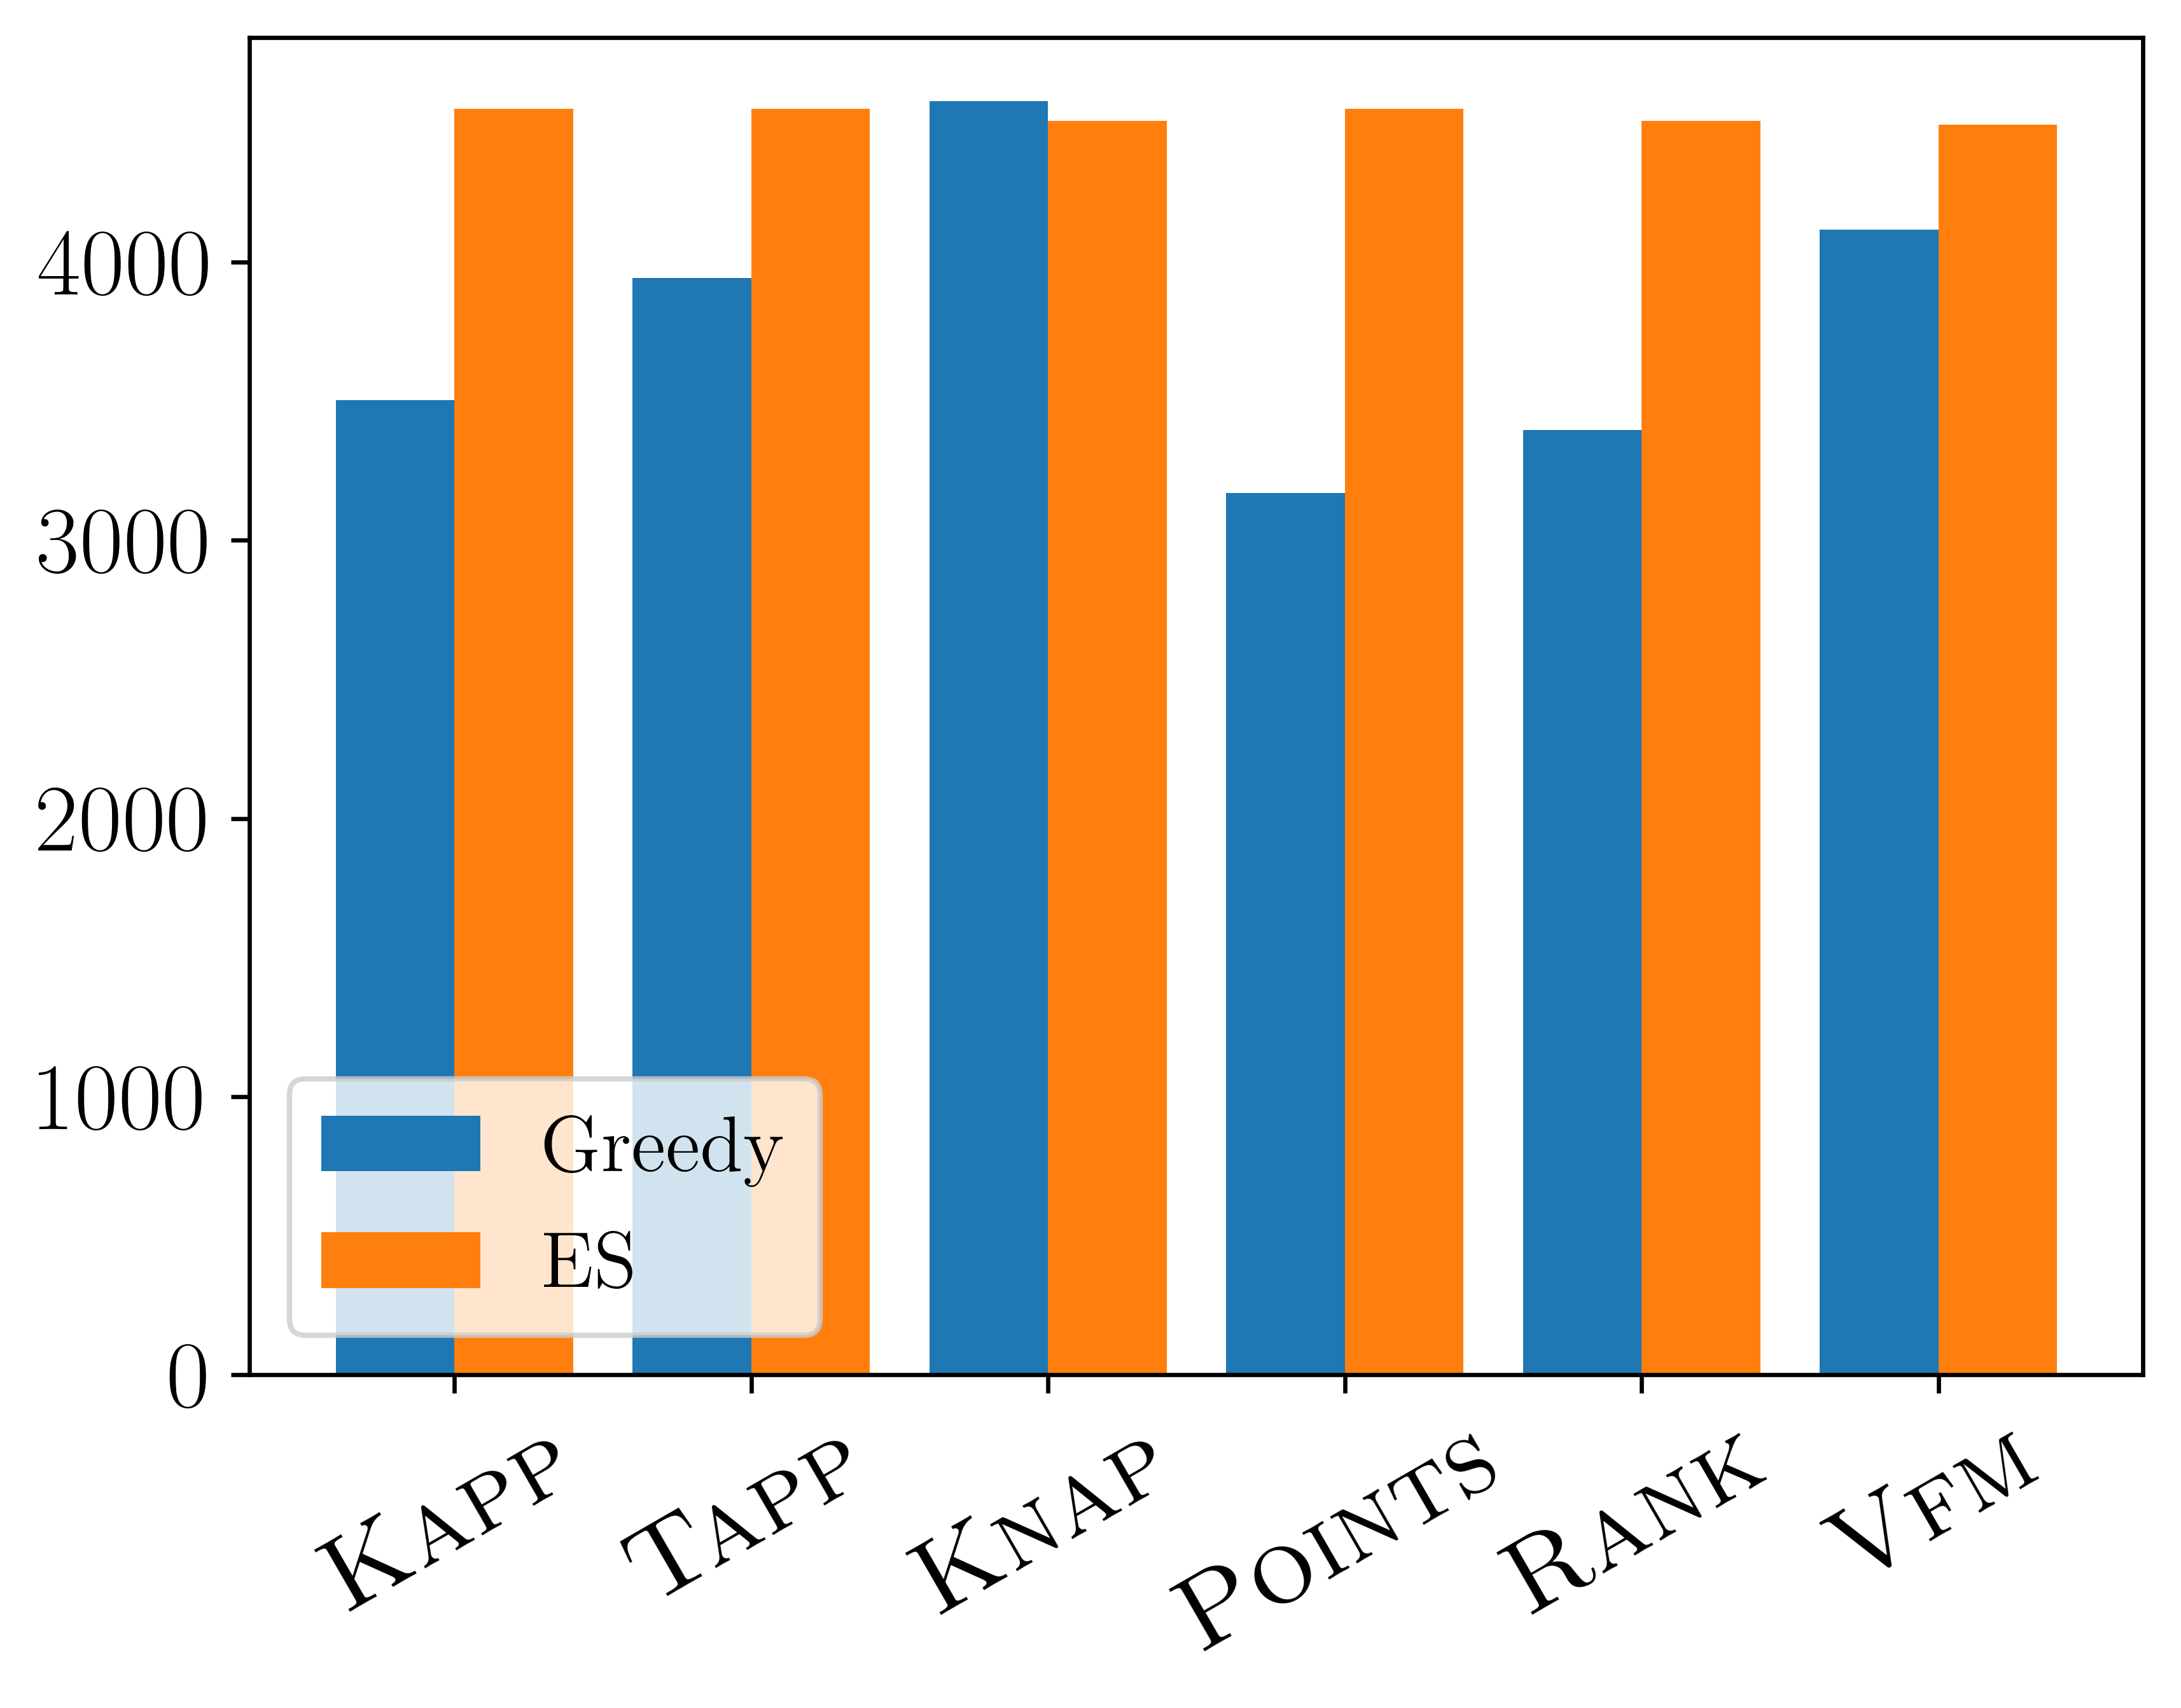
\includegraphics[width=7.5cm]{experiment/Ranking_value_money_welfare.png}
% \caption{Average social welfare (averaged across elections) using \vfm{}-voters to compute welfare.
% }\label{fig:vfm_welfare}
% \end{center}
% \end{figure}

% \begin{figure}[!ht]
% \begin{center}
% 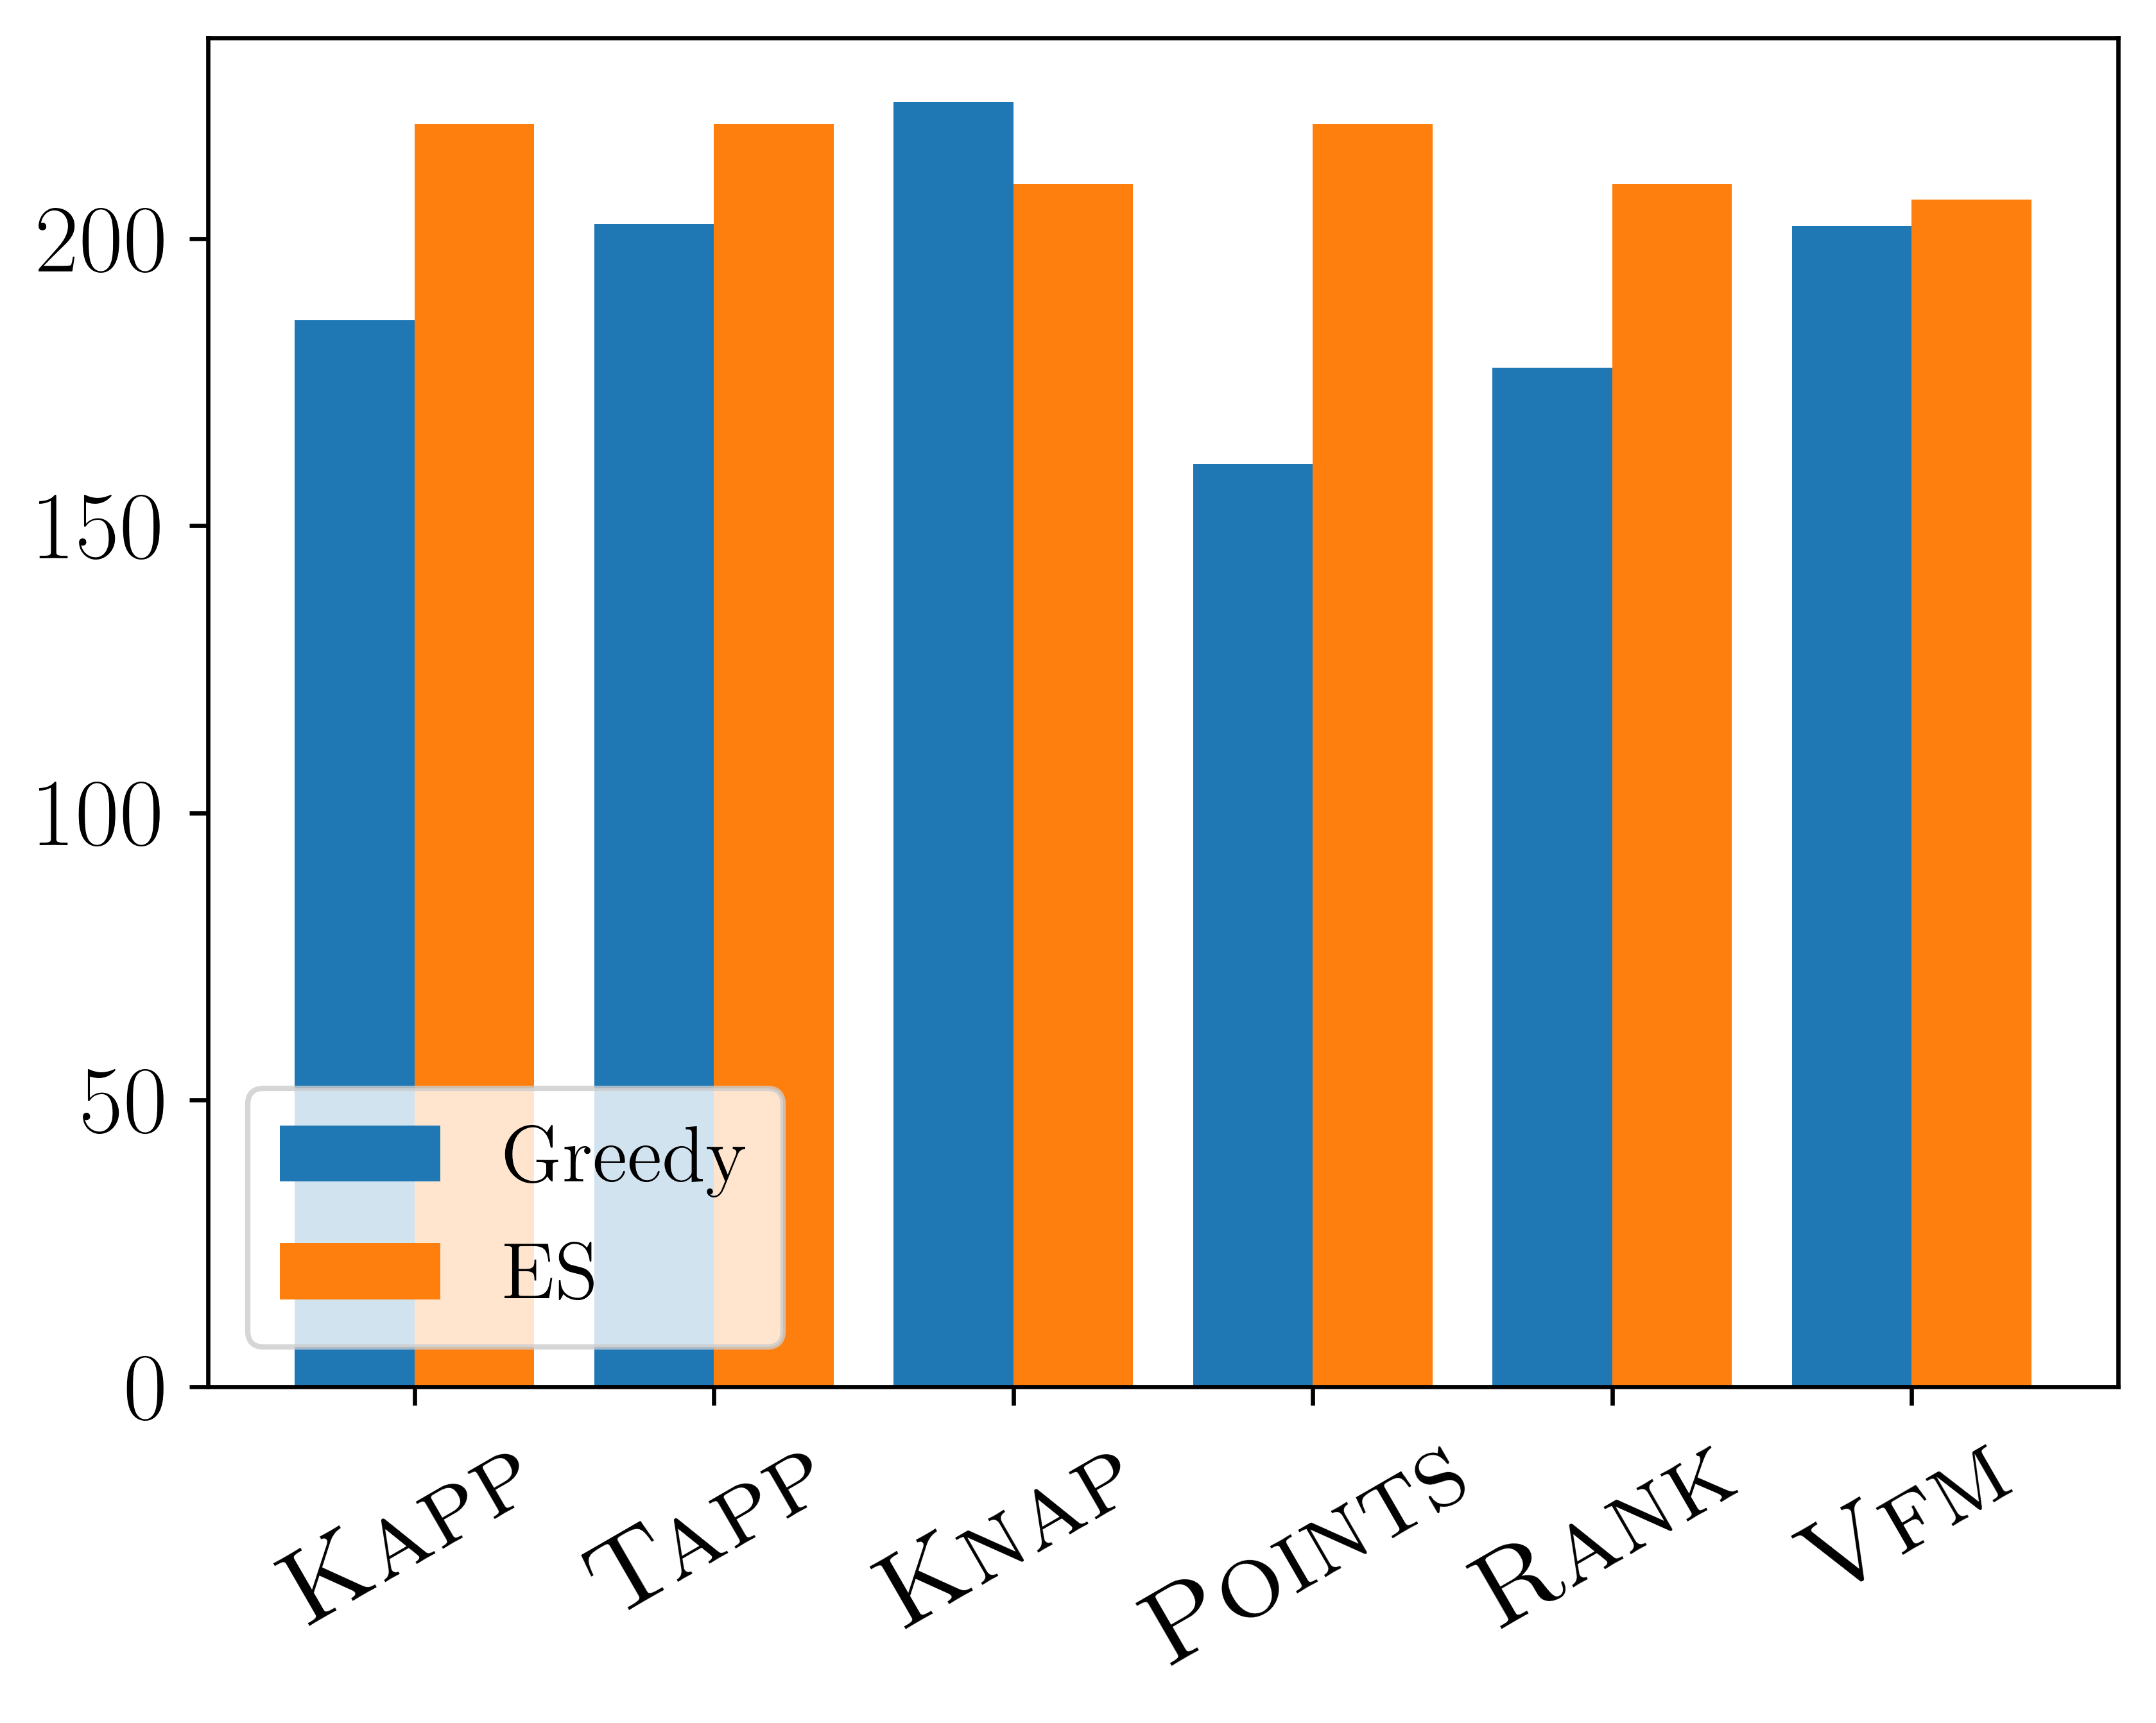
\includegraphics[width=7.5cm]{experiment/Threshold_welfare.png}
% \caption{Average social welfare (averaged across elections) using \tapp{}-voters to compute welfare.
% }\label{fig:tapp_welfare}
% \end{center}
% \end{figure}

% \begin{figure}[ht]
% \begin{center}
% 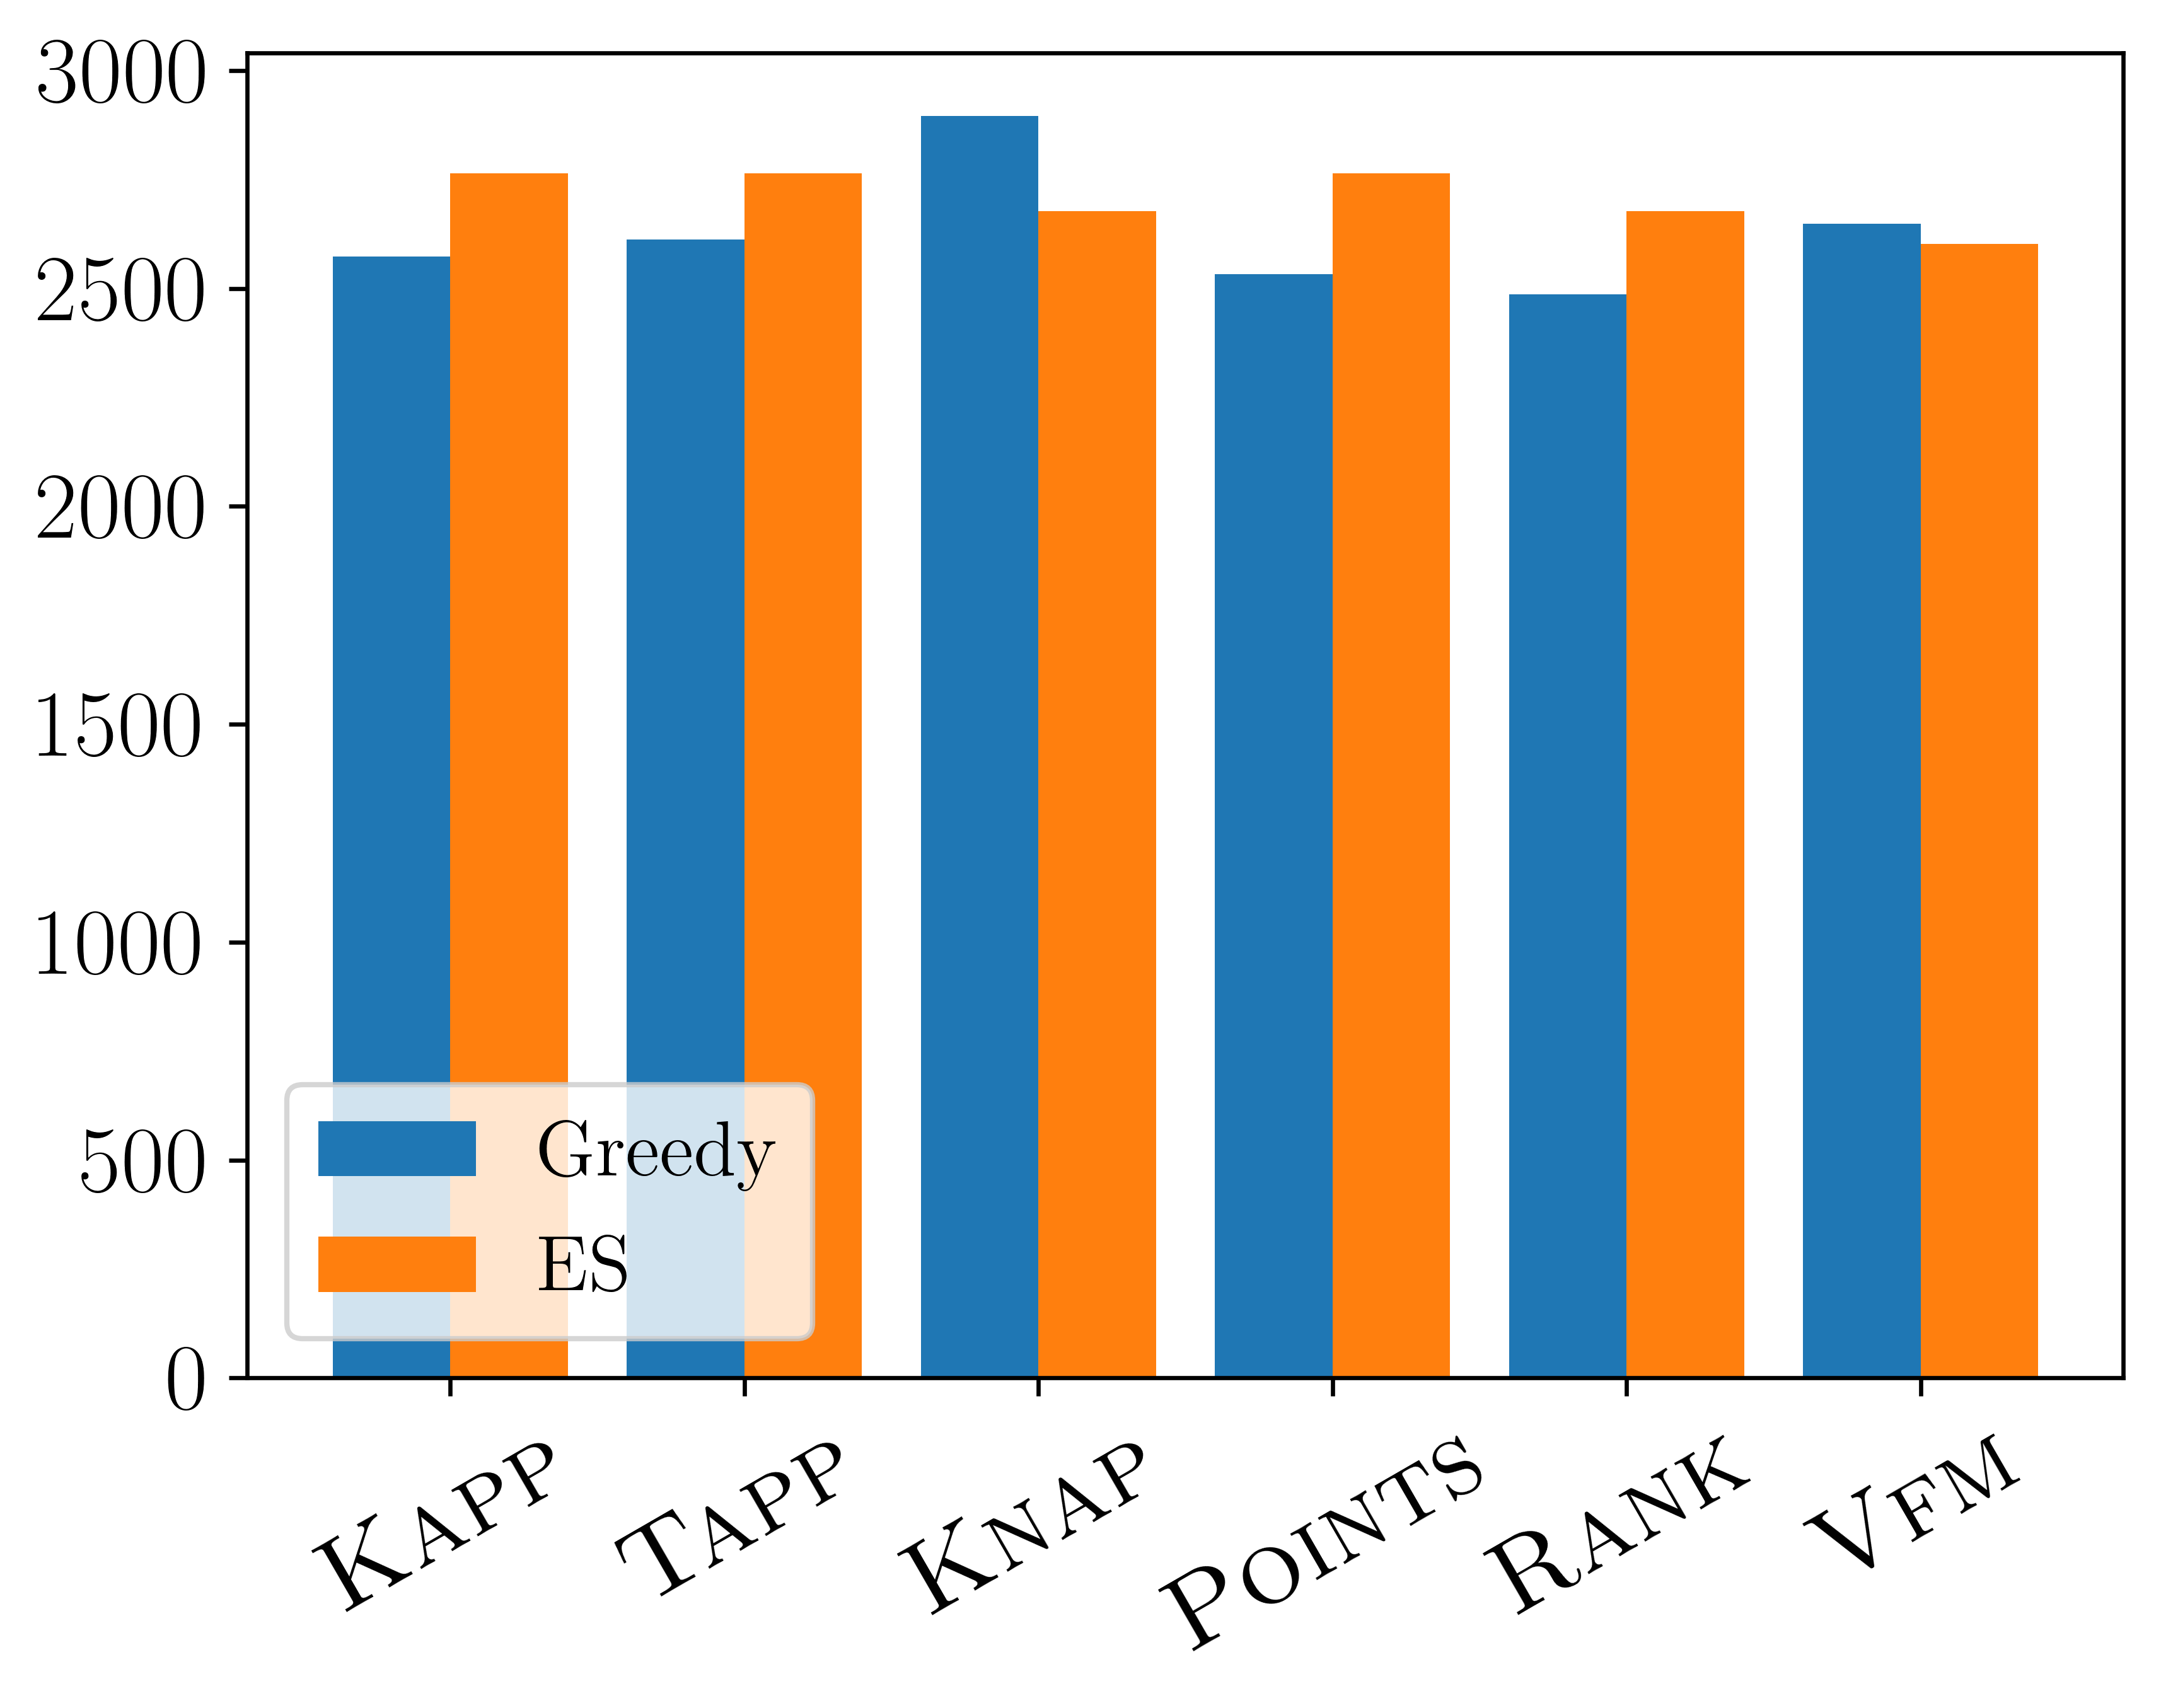
\includegraphics[width=7.5cm]{experiment/Utilities_welfare.png}
% \caption{Average social welfare (averaged across elections) using \points{}-voters to compute welfare.
% }\label{fig:util_welfare}
% \end{center}
% \end{figure}

\begin{figure*}[ht]
     \centering
          \begin{subfigure}[b]{0.45\textwidth}
         \centering
       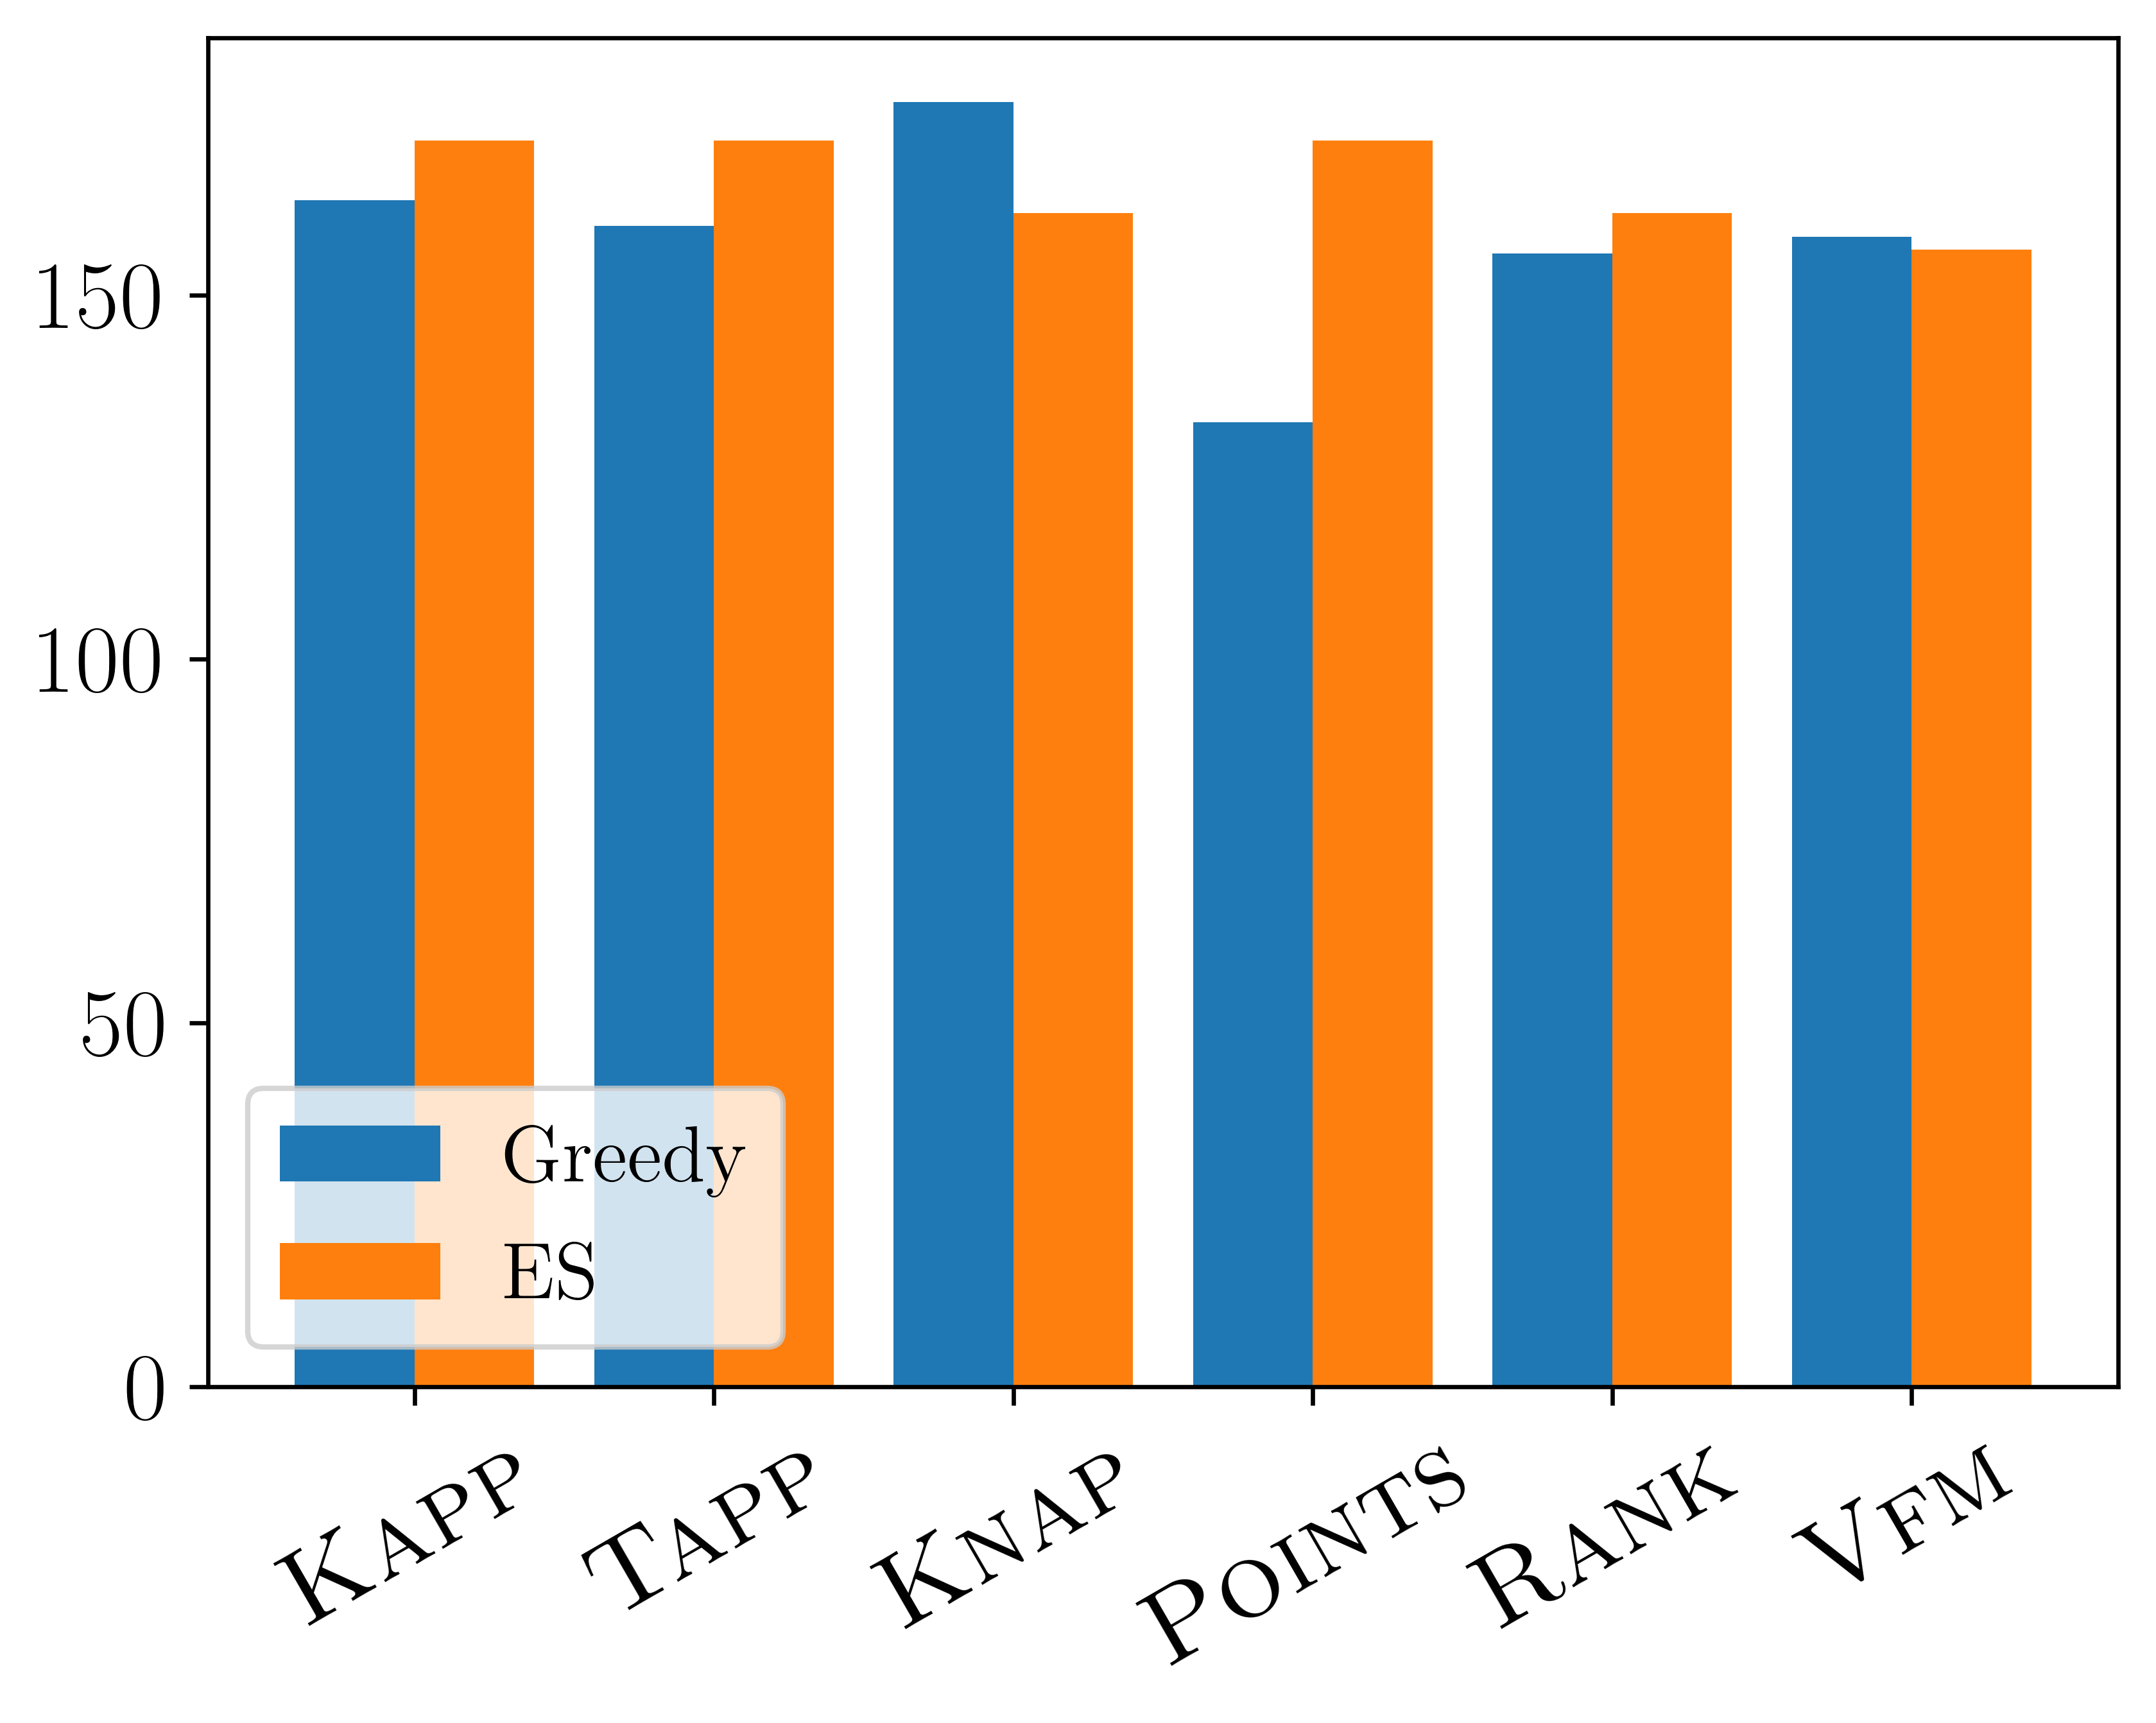
\includegraphics[width=6cm]{experiment/k_approval_welfare.png}
\caption{Average social welfare (averaged across elections) using \kapp{}-voters to compute welfare.
}\label{fig:kapp_welfare}
     \end{subfigure}\hfill
     \begin{subfigure}[b]{0.45\textwidth}
         \centering
         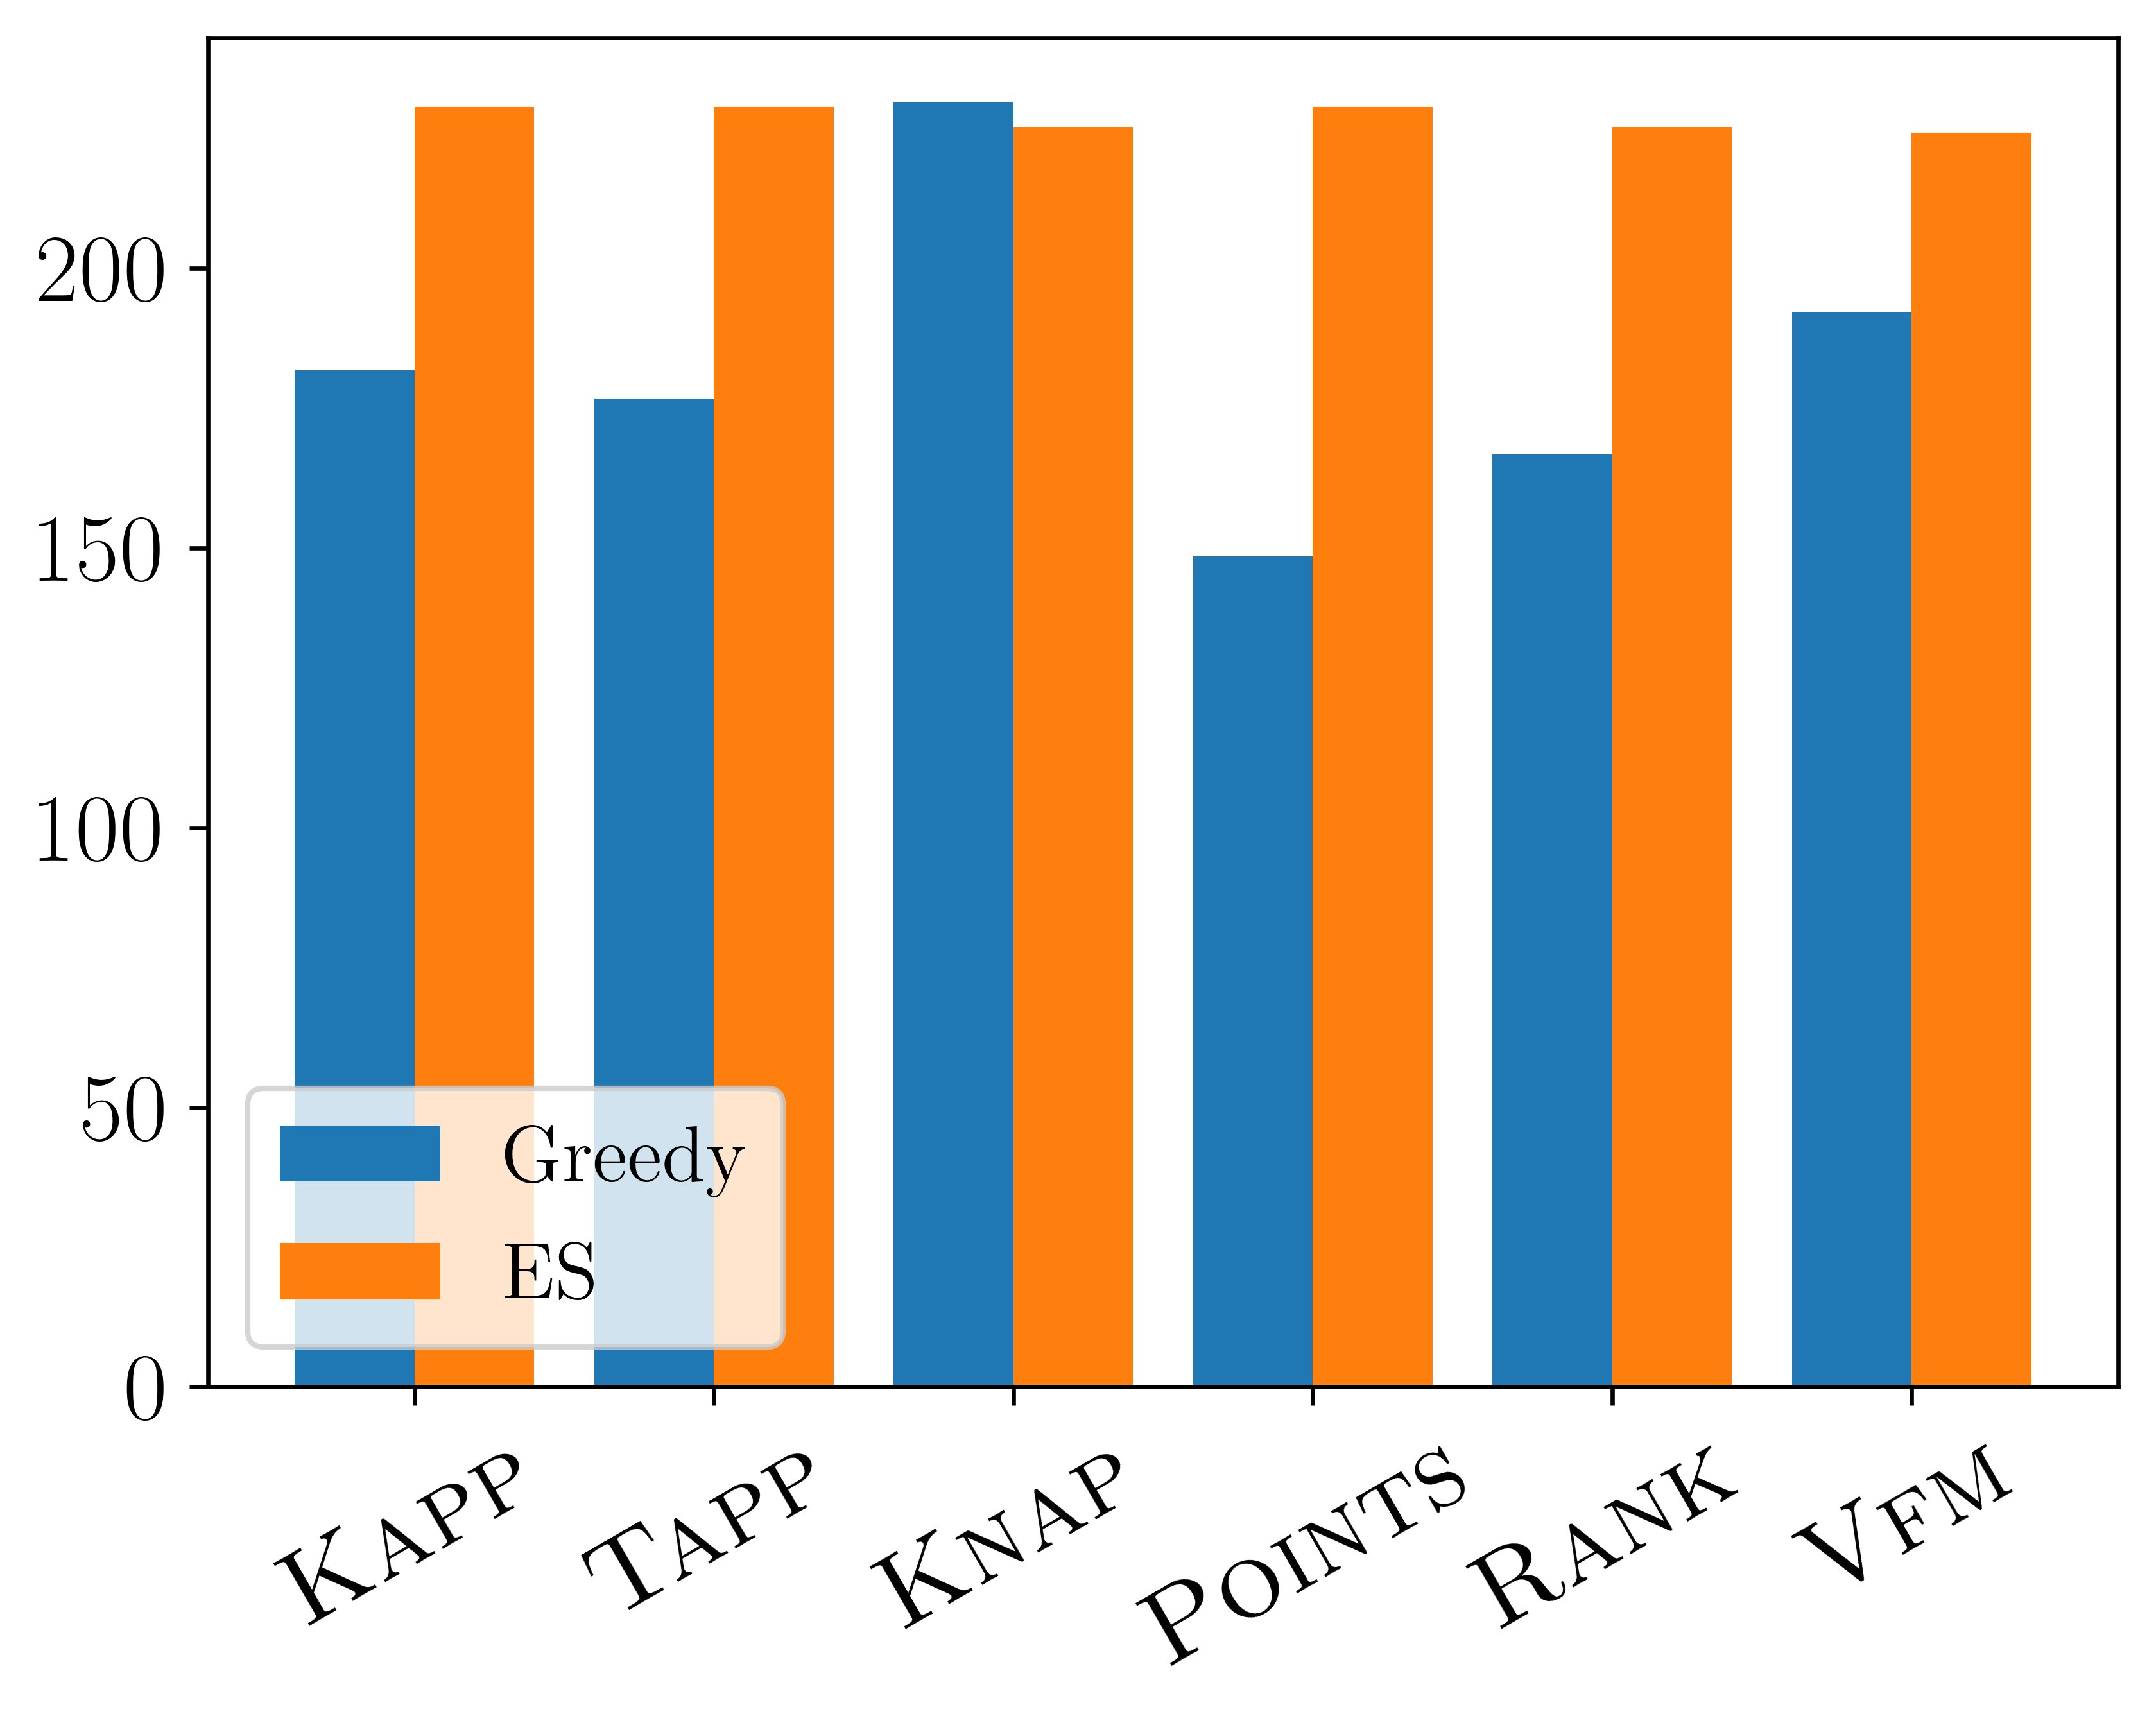
\includegraphics[width=6cm]{experiment/Knapsack_welfare.png}
\caption{Average social welfare (averaged across elections) using \knap{}-voters to compute welfare.
}\label{fig:knap_welfare}
     \end{subfigure}
     \hfill
     \begin{subfigure}[b]{0.45\textwidth}
         \centering
         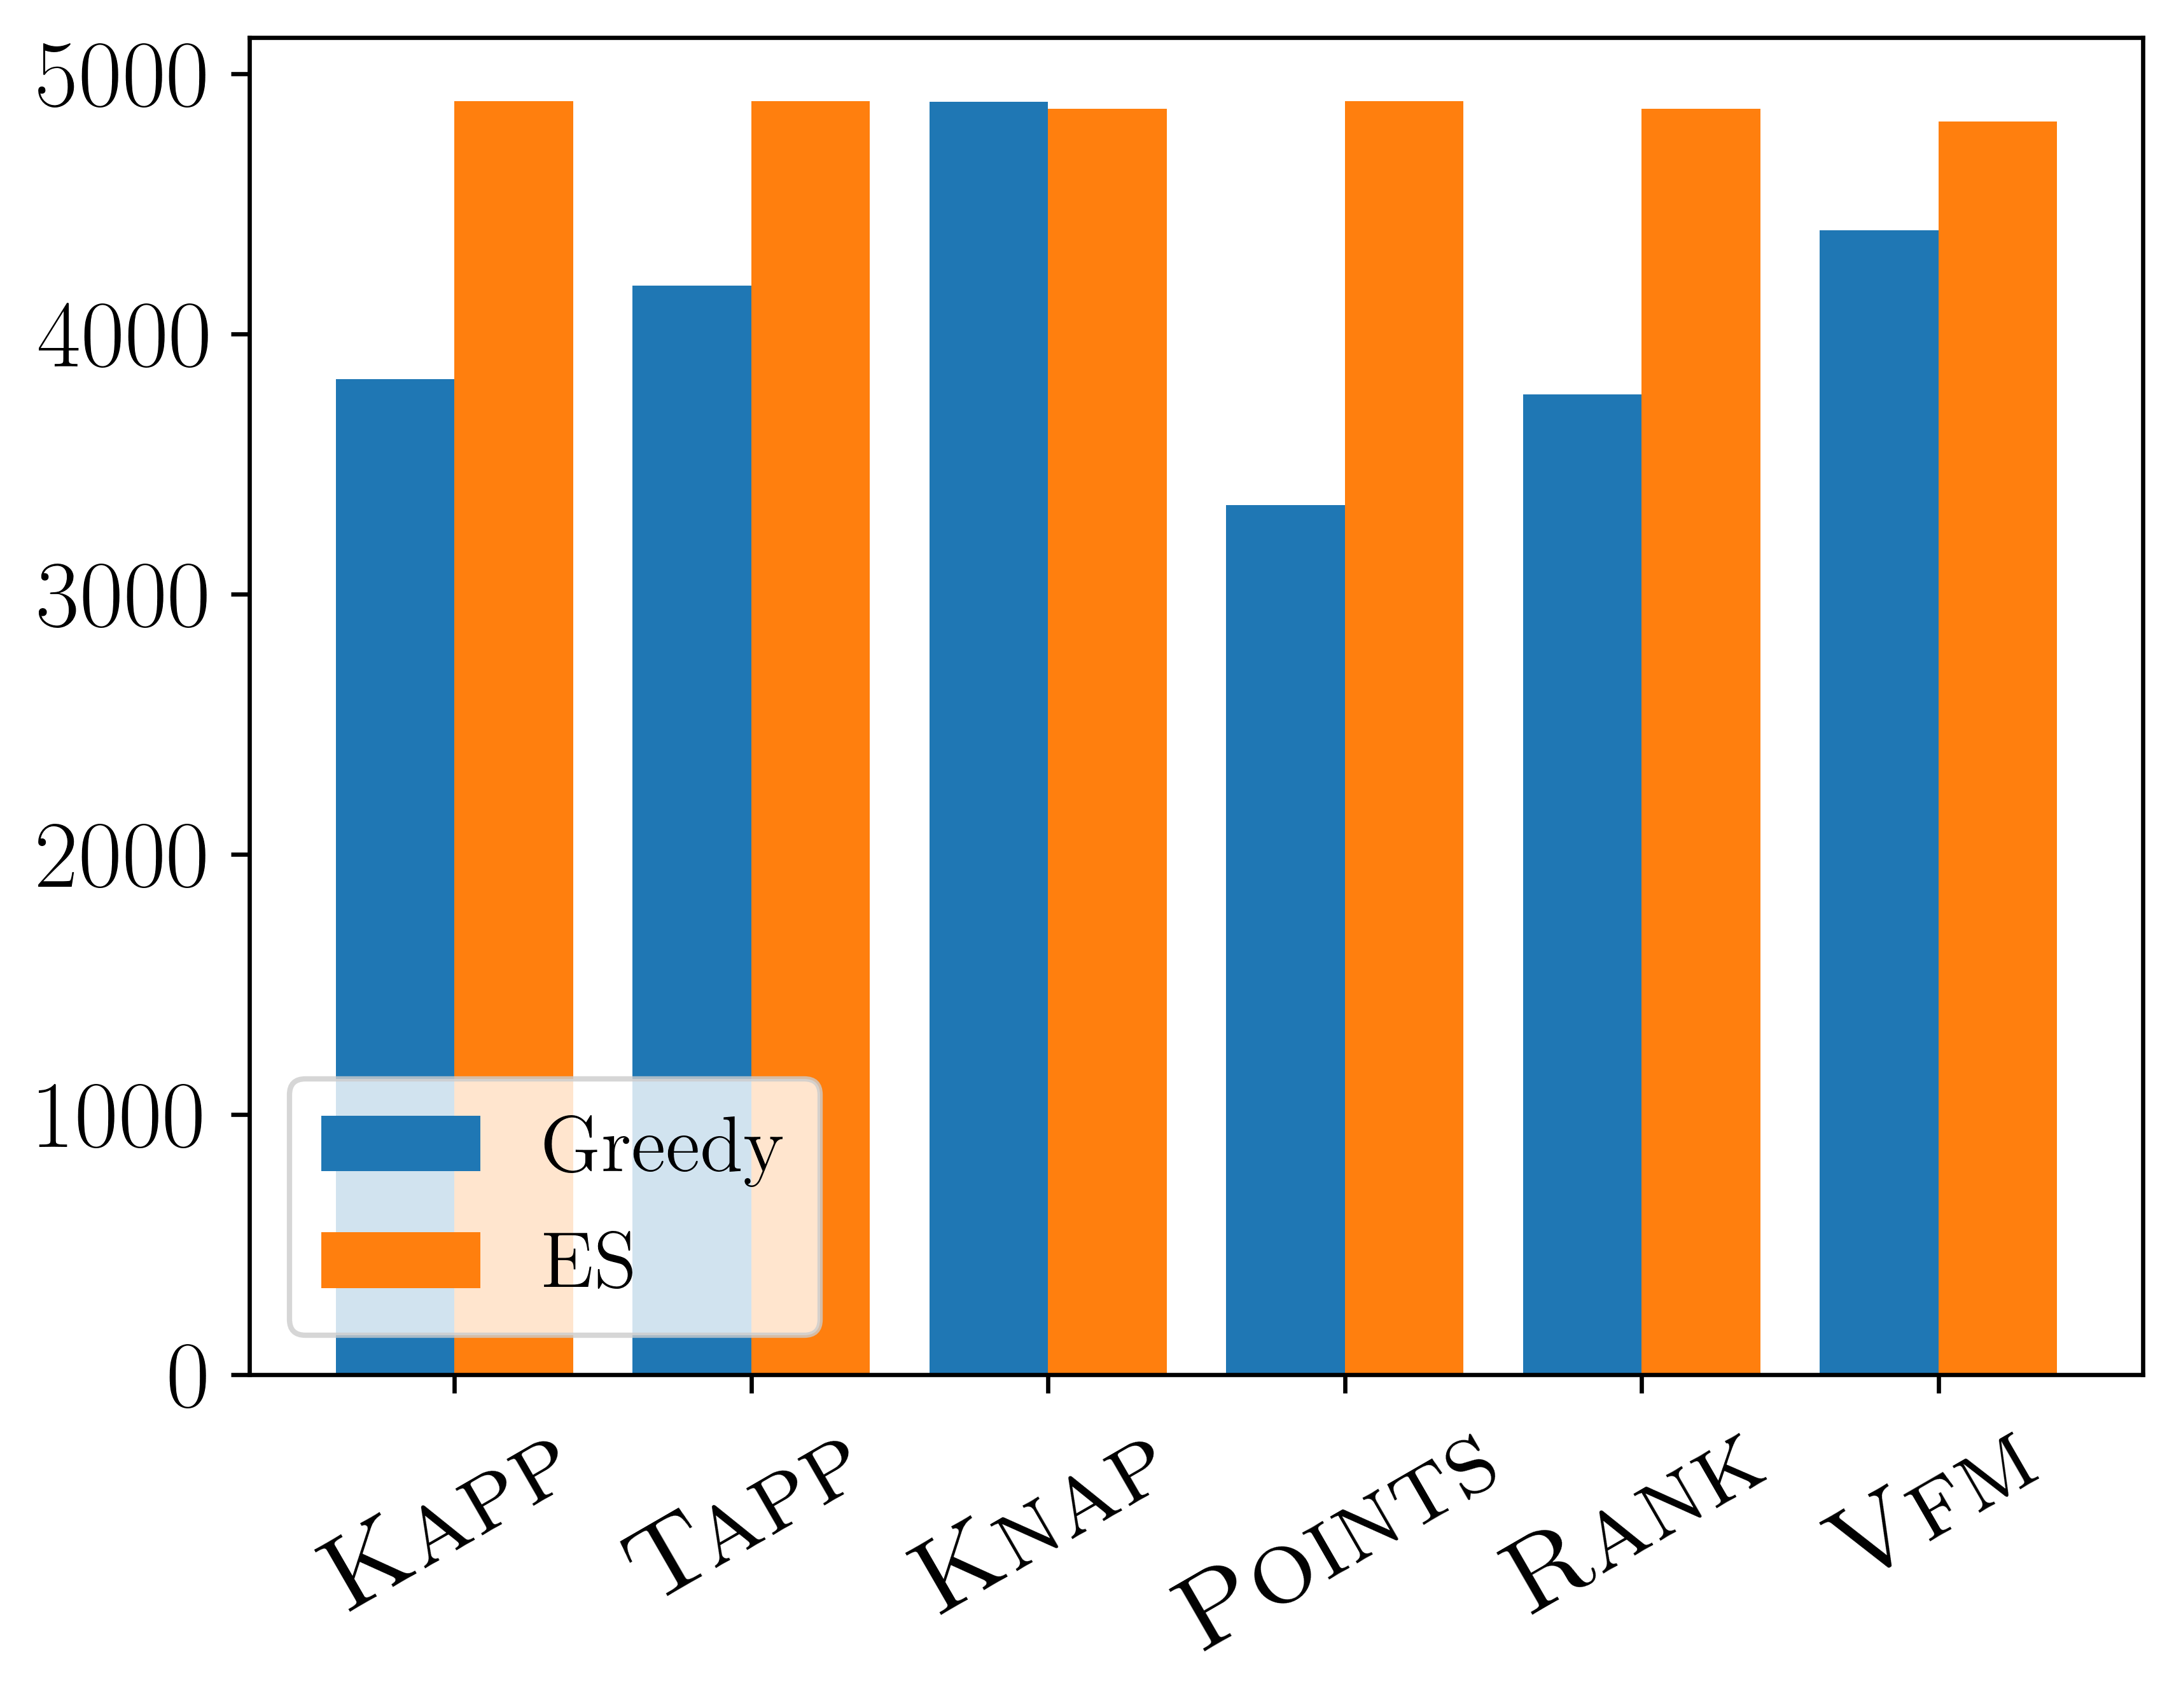
\includegraphics[width=6cm]{experiment/Ranking_value_welfare.png}
\caption{Average social welfare (averaged across elections) using \rank{}-voters to compute welfare.
}\label{fig:rank_welfare}
     \end{subfigure}
     \hfill
     \begin{subfigure}[b]{0.45\textwidth}
         \centering
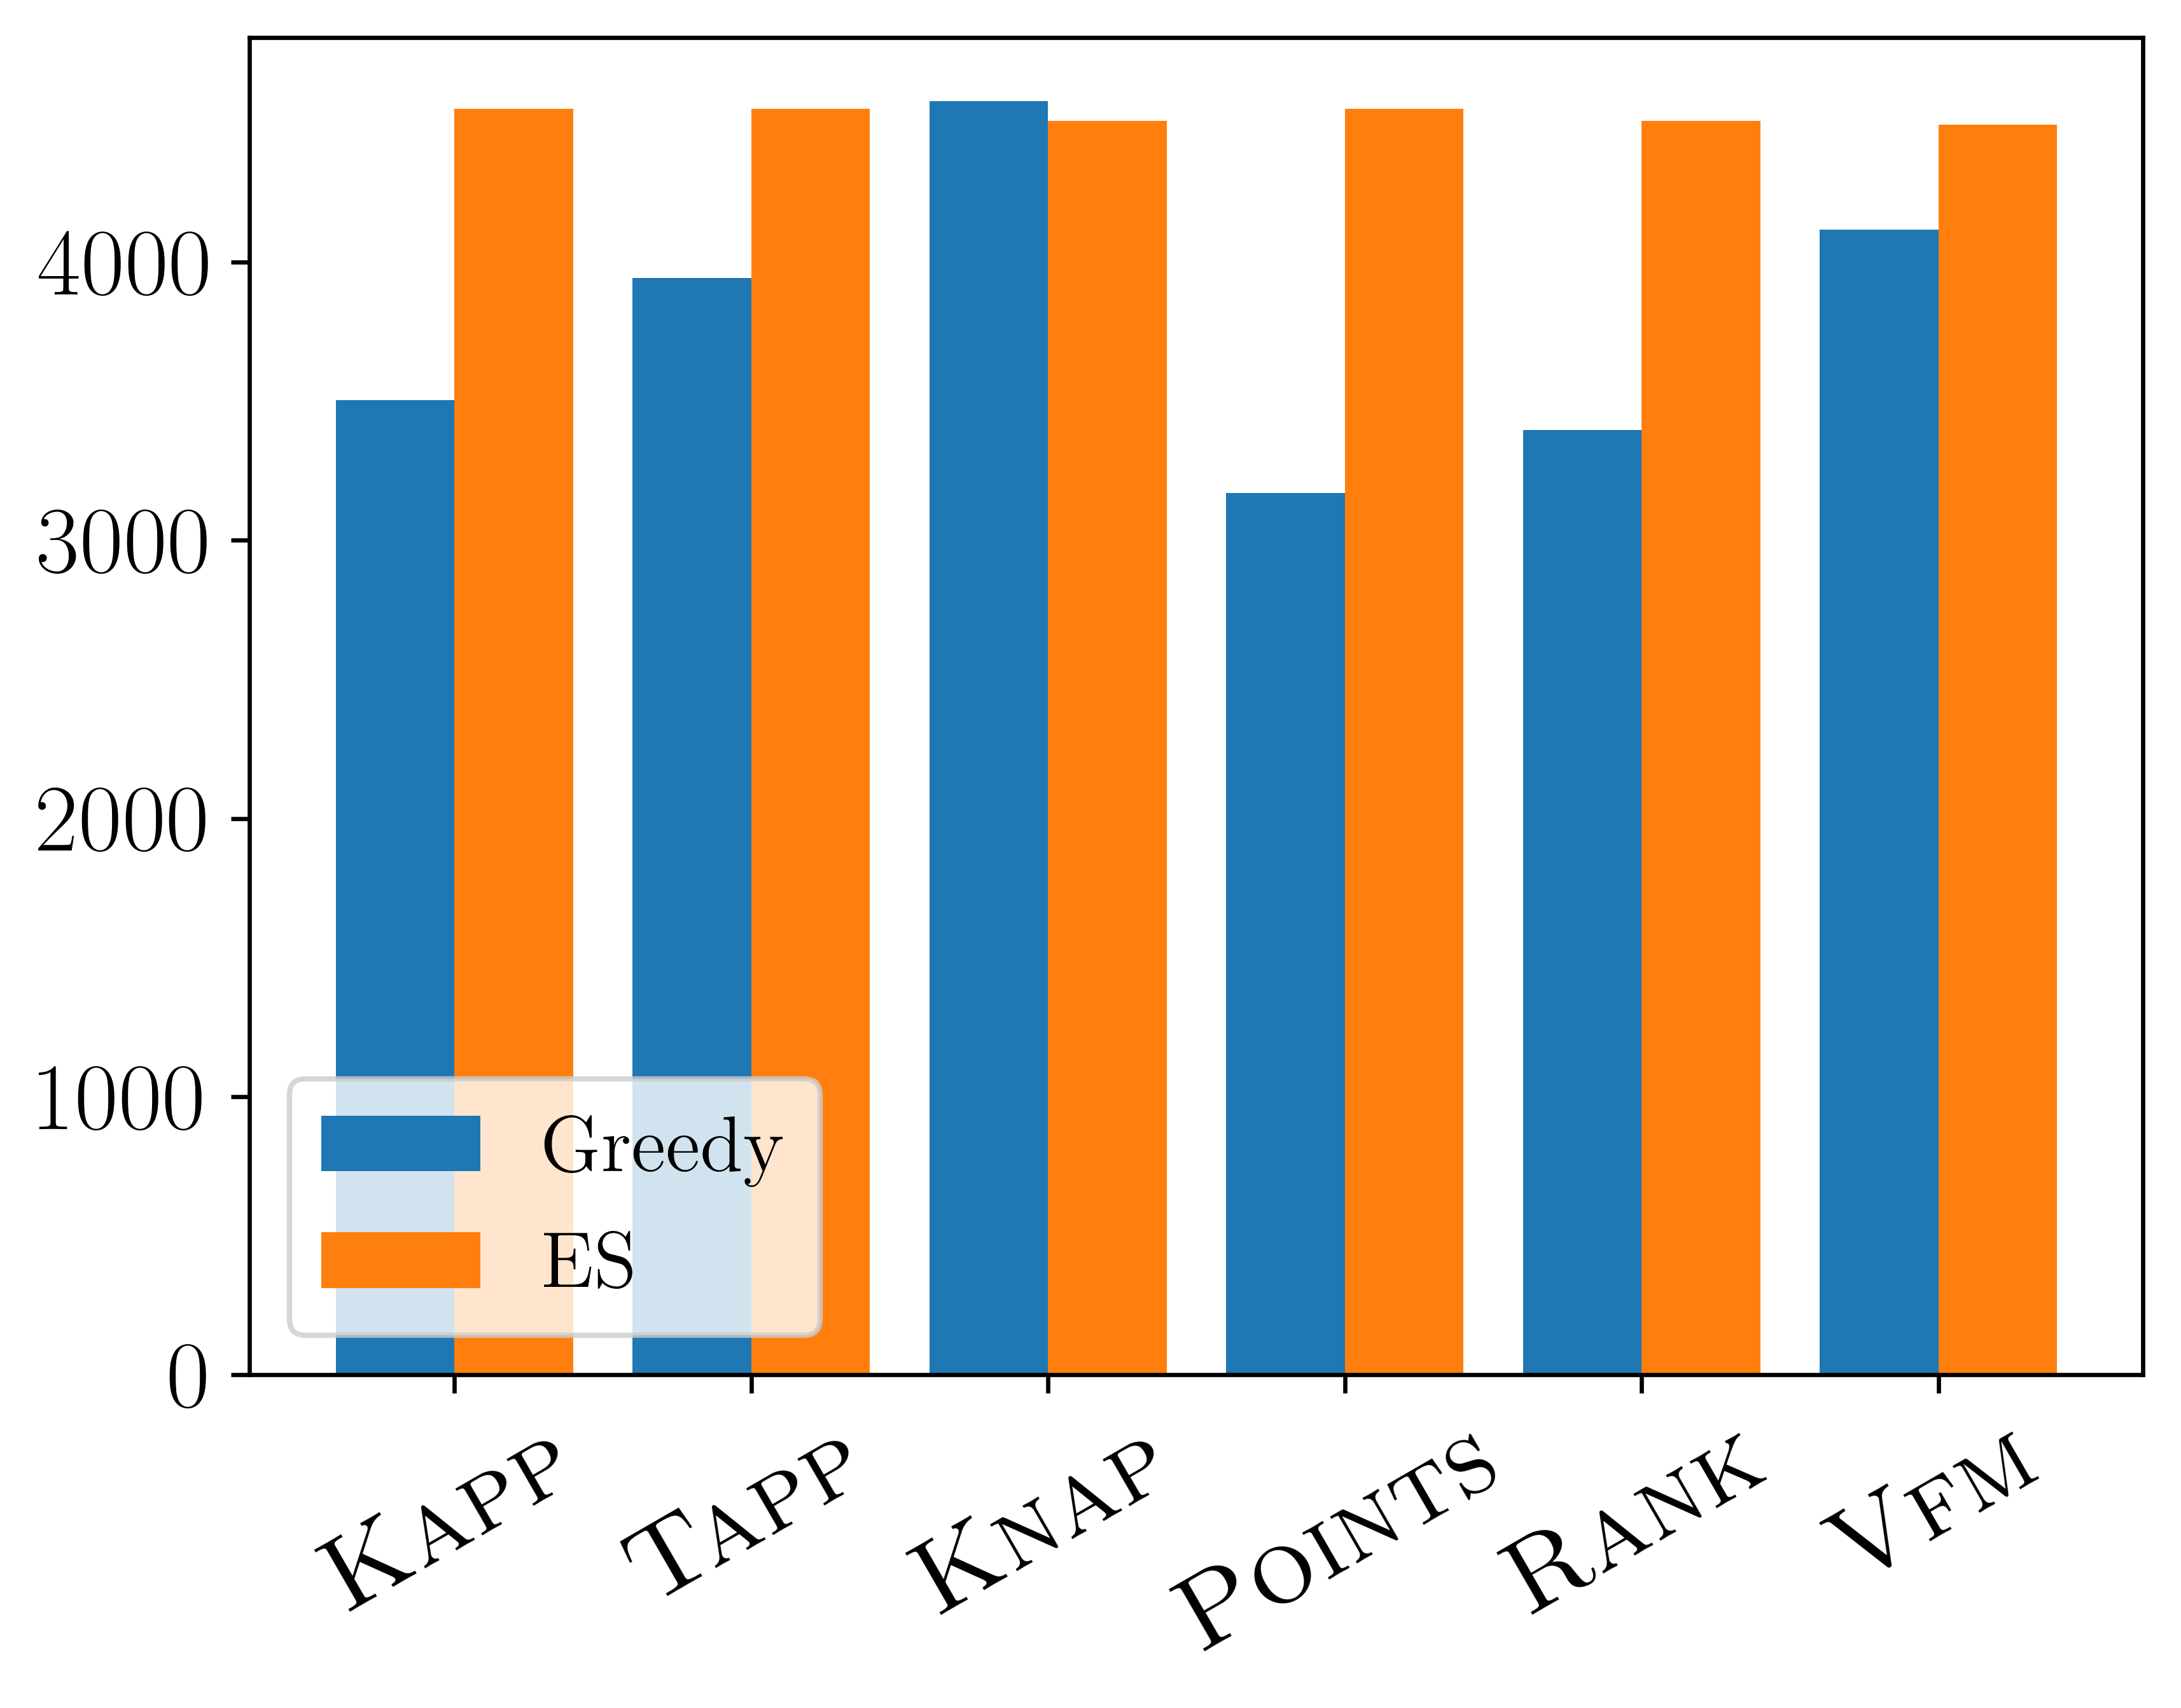
\includegraphics[width=6cm]{experiment/Ranking_value_money_welfare.png}
\caption{Average social welfare (averaged across elections) using \vfm{}-voters to compute welfare.
}\label{fig:vfm_welfare}
     \end{subfigure}
     \begin{subfigure}[b]{0.45\textwidth}
         \centering
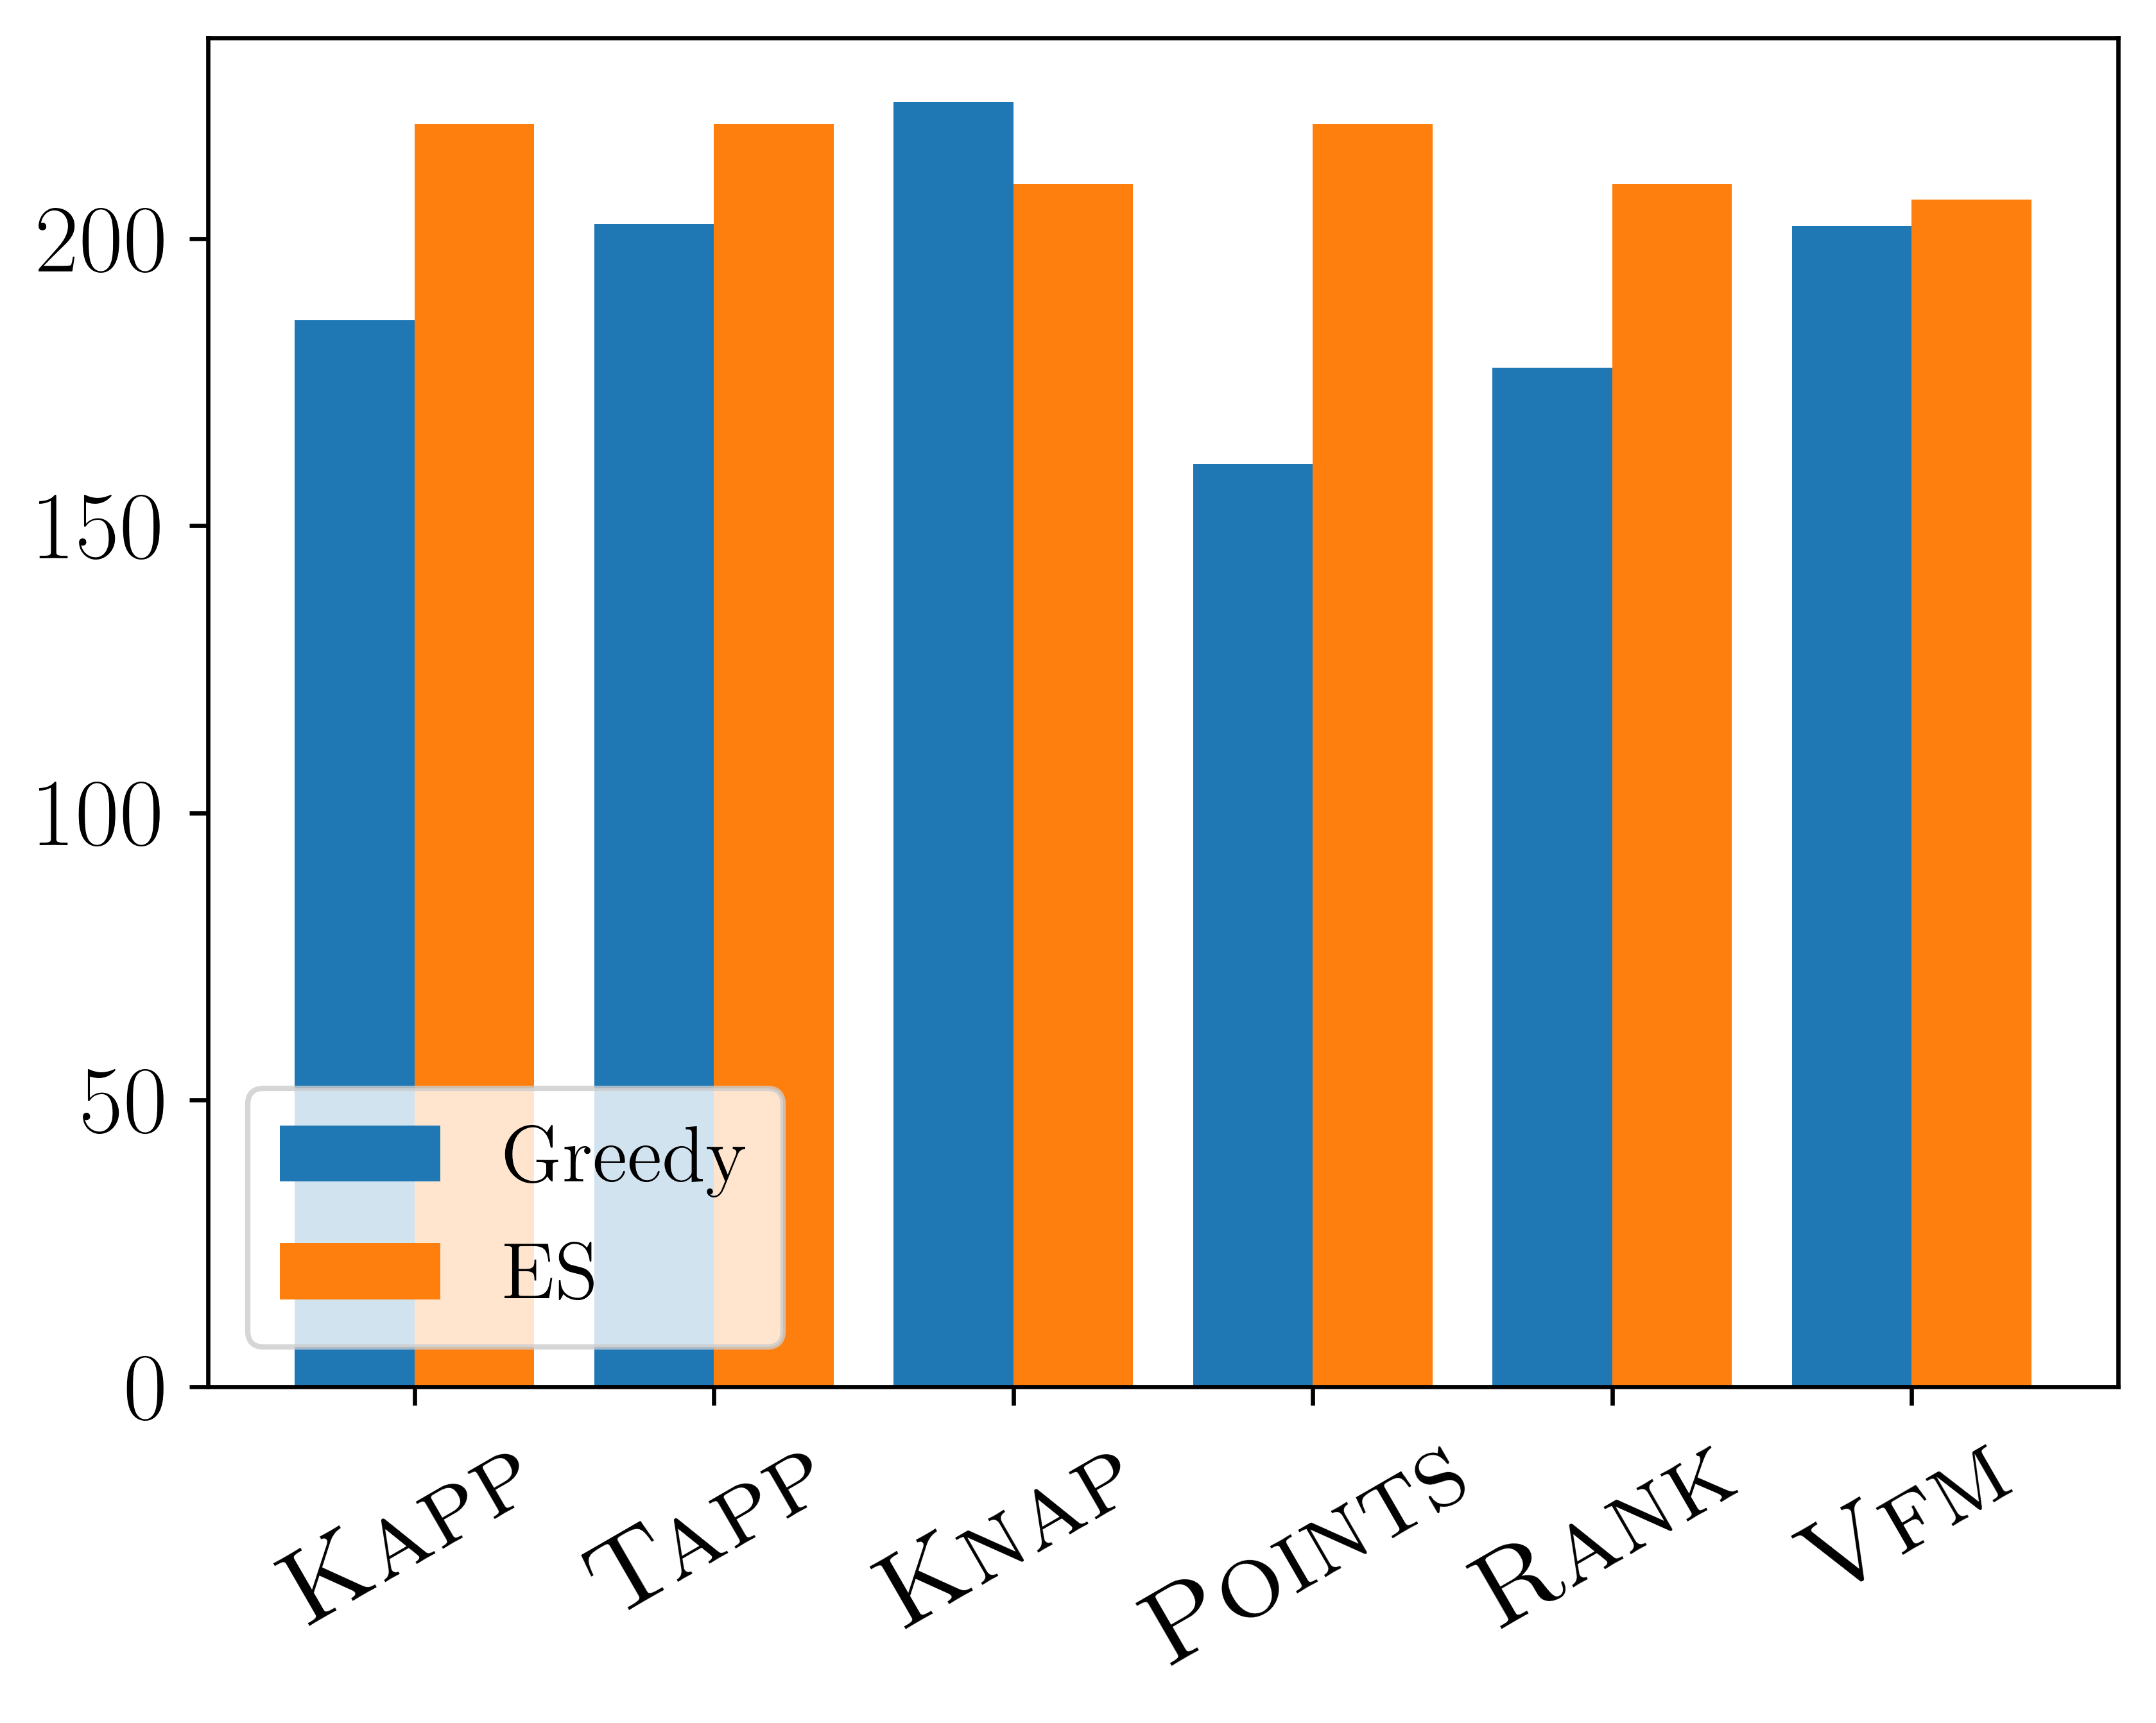
\includegraphics[width=6cm]{experiment/Threshold_welfare.png}
\caption{Average social welfare (averaged across elections) using \tapp{}-voters to compute welfare.
}\label{fig:tapp_welfare}
     \end{subfigure}
     \hfill
     \begin{subfigure}[b]{0.45\textwidth}
         \centering
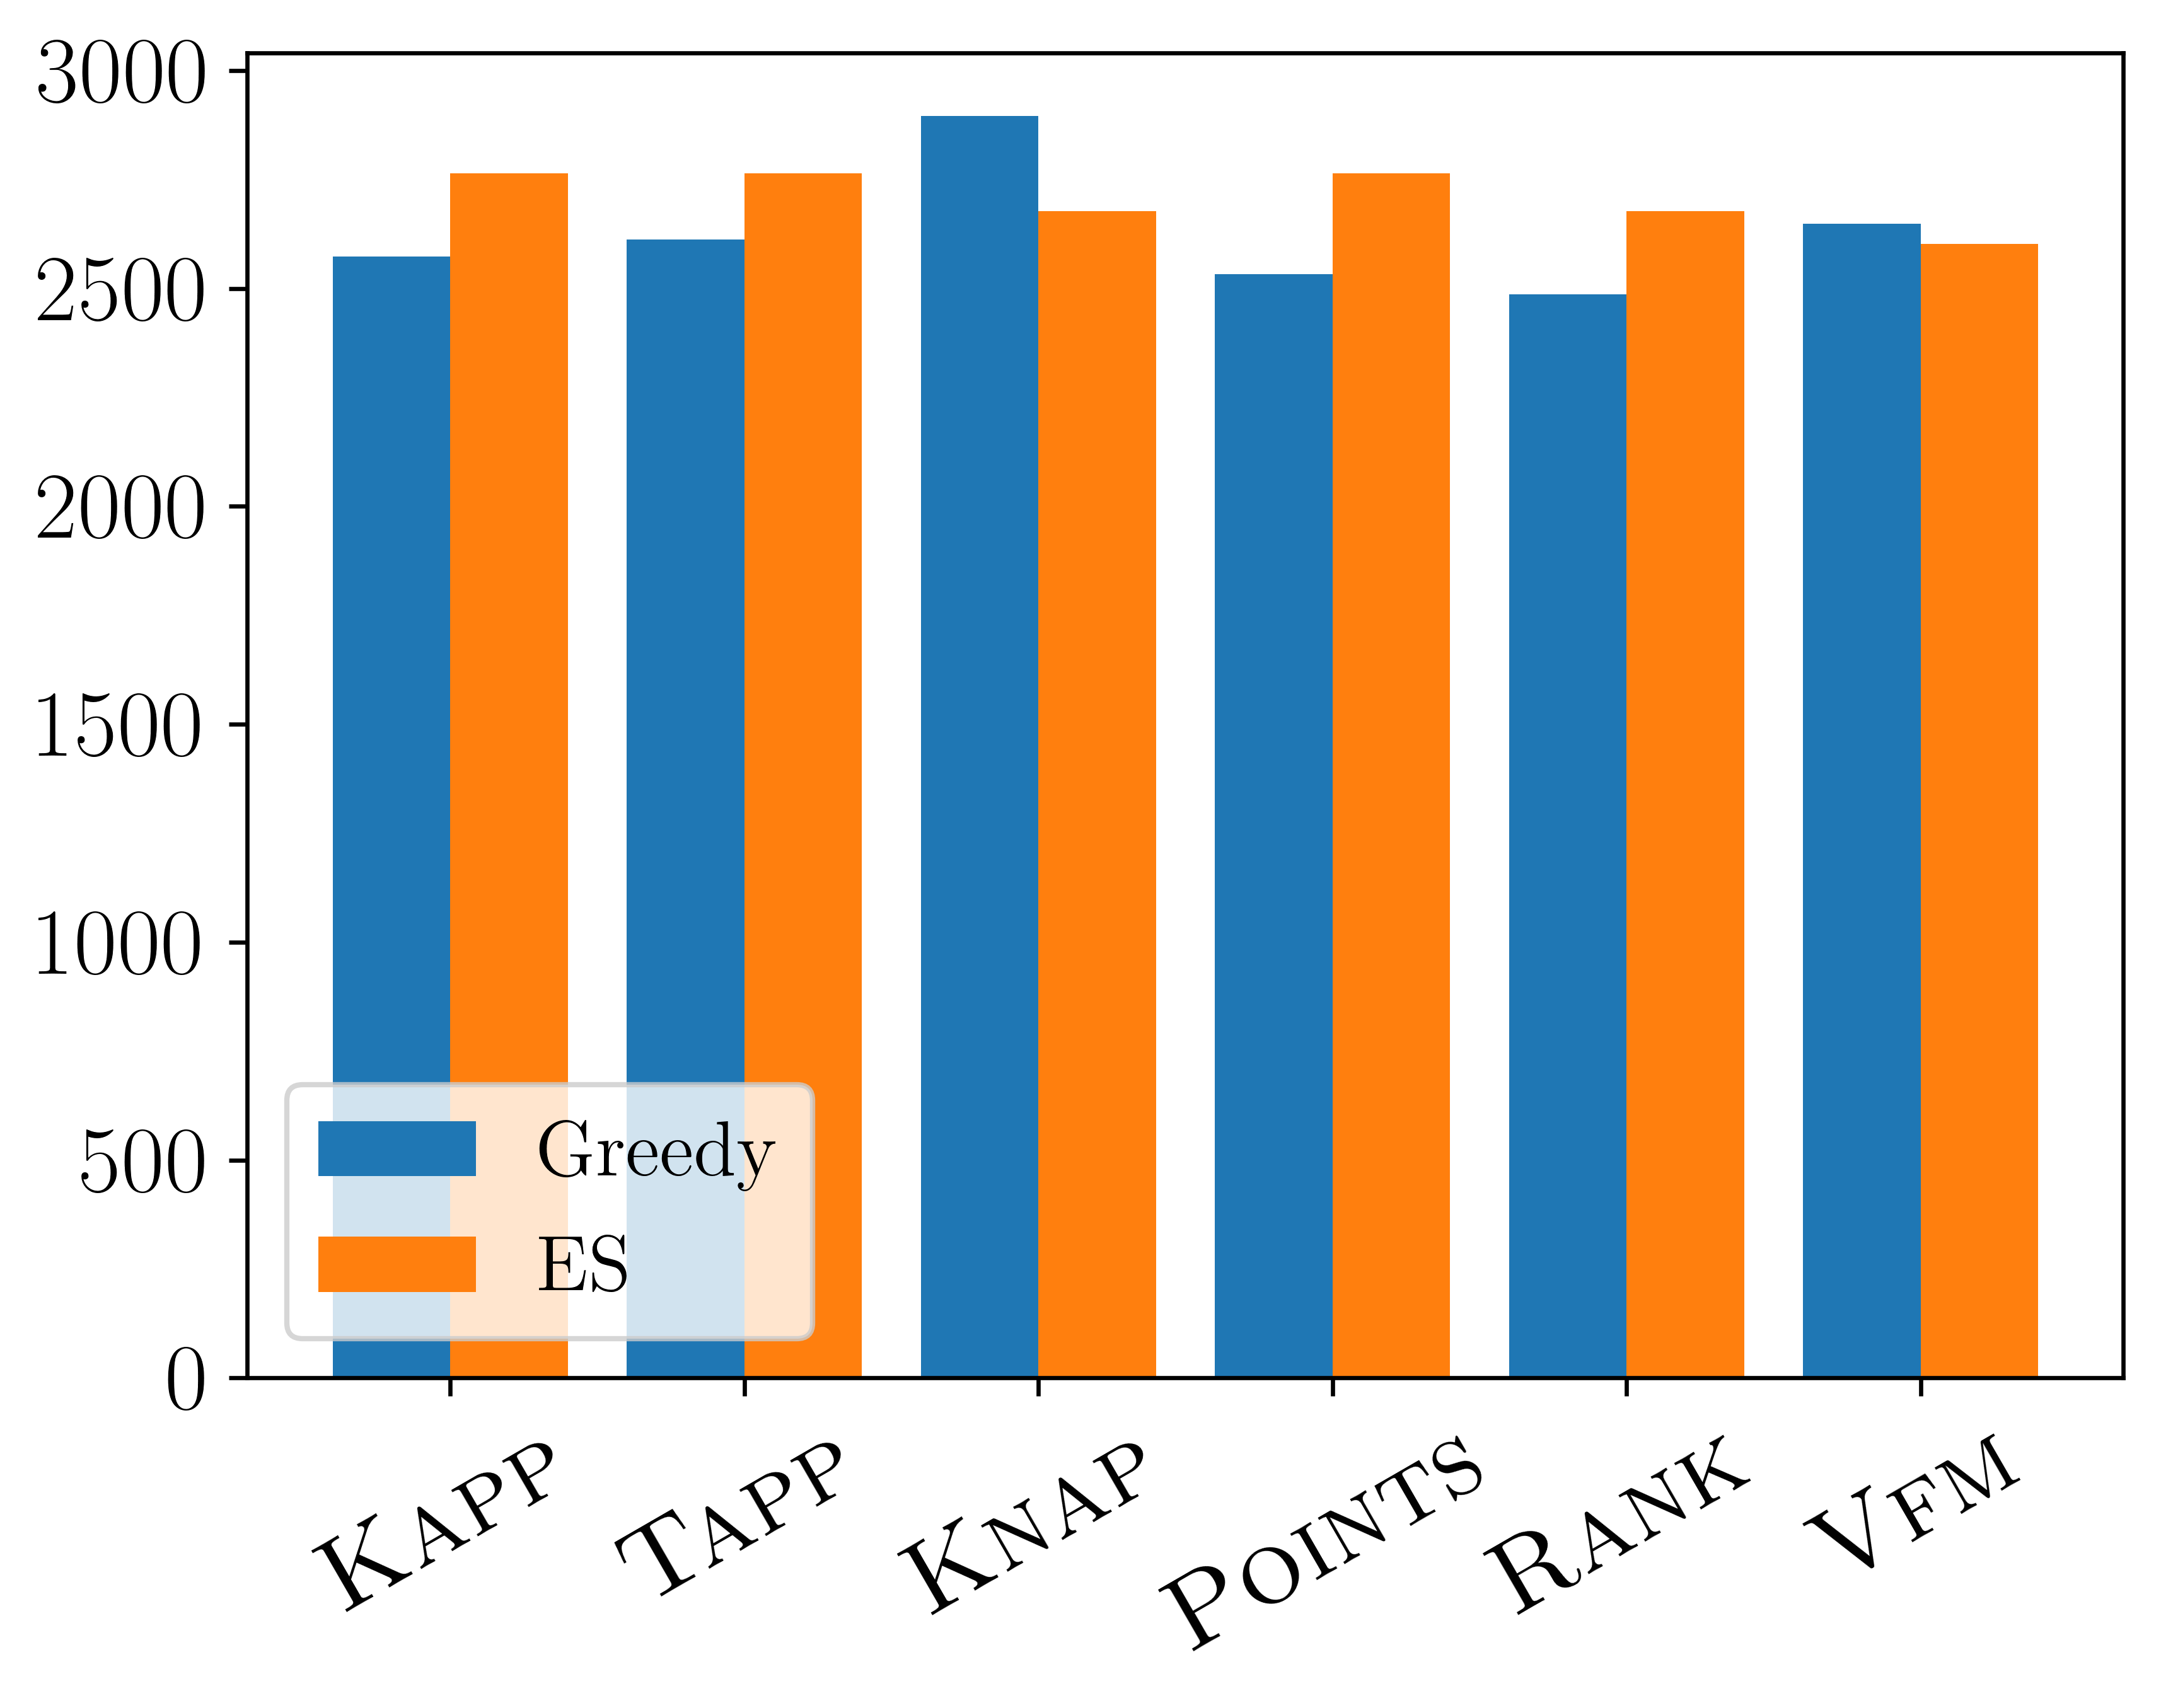
\includegraphics[width=6cm]{experiment/Utilities_welfare.png}
\caption{Average social welfare (averaged across elections) using \points{}-voters to compute welfare.
}\label{fig:util_welfare}
     \end{subfigure}
     

        \caption{Welfare.}
        \label{fig:entropy:app}
\end{figure*}

%%%%%%%%%%%%%%%%%%%%%%%%%%%%%%%%%%%%%%%%%%%%%%%%%%%%%%%%%%%%%%%%%%%%%%%%%

\end{document}

%%%%%%%%%%%%%%%%%%%%%%%%%%%%%%%%%%%%%%%%%%%%%%%%%%%%%%%%%%%%%%%%%%%%%%%%%